\documentclass[openright,diss]{deletex}

\usepackage[T1]{fontenc}
\usepackage[latin1]{inputenc}
\usepackage{amsthm,pifont,amsfonts,amssymb,amsmath,graphicx,float,url,enumerate}
%\usepackage[dvips,ps2pdf]{hyperref}

\newcommand\real{\mathbb{R}}
\newcommand{\req}[1]{(\ref{#1})}

\newcounter{defin}
\newcounter{teorem}
\newtheorem{definition}{Defini��o\refstepcounter{defin}}
\newtheorem{theorem}{Teorema\refstepcounter{teorem}}

\DeclareMathOperator{\sen}{sen}
\DeclareMathOperator{\inv}{inv}
\DeclareMathOperator{\sign}{sign}
\DeclareMathOperator{\atan}{atan2}

\newenvironment{margins}[2]{\begin{list}{}{\setlength{\leftmargin}{#1}\setlength{\rightmargin}{#2}}\item}{\end{list}}

\title{Controle Preditivo de Rob�s M�veis N�o Holon�micos}

\author{K�hne}{Felipe}

\advisorwidth{.66\linewidth}

\advisor[Prof.~Dr.]{Gomes da Silva Jr.}{Jo�o Manoel}
\advisorinfo{UFRGS}{Doutor pela Universidade Paul Sabatier -- Toulouse, Fran�a}
\coadvisor[Prof.~Dr.]{Fetter Lages}{Walter}
\coadvisorinfo{UFRGS}{Doutor pelo Instituto Tecnol�gico de Aeron�utica -- S�o Jos� dos Campos, Brasil}

\examiner[Prof.~Dr.]{Normey-Rico}{Julio Elias}
\examinerinfo{UFSC}{Doutor pela Universidade de Sevilla -- Sevilla, Espanha}
\examiner[Prof.~Dr.]{Trierweiler}{Jorge Ot�vio}
\examinerinfo{UFRGS}{Doutor pela Universidade de Dortmund -- Dortmund, Alemanha}
\examiner[Prof.~Dr.]{Reginatto}{Romeu}
\examinerinfo{UFRGS}{Doutor pela Universidade Federal de Santa Catarina, UFSC}
\examiner[Prof.~Dr.]{Sanfelice Bazanella}{Alexandre}
\examinerinfo{UFRGS}{Doutor pela Universidade Federal de Santa Catarina, UFSC}

\date{mar�o}{2005}

% iniciar todas com letras min�sculas, exceto no caso de abreviaturas
\keyword{sistemas n�o holon�micos}
\keyword{rob�s m�veis}
\keyword{controle preditivo baseado em modelo}


%%%%%%%%%%%%%%%%
\begin{document}


% Inclui \maketitle, dedicat�ria, agradecimentos, resumo e abstract, sum�rio, lista de figuras, tabelas, abreviaturas e s�mbolos
\maketitle

\chapter*{Dedicat�ria}
Aos meus pais Jo�o e Elisabeth e � minha namorada Luciana.

\chapter*{Agradecimentos}
Gostaria de deixar aqui meus profundos agradecimentos ao meu orientador, Prof. Jo�o Manoel, e ao meu co-orientador, Prof. Walter, pela inspira��o, amizade e constante disponibilidade durante todo o curso de mestrado.

Ao Programa de P�s-Gradua��o em Engenharia El�trica, PPGEE, pela oportunidade de realiza��o de trabalhos em minha �rea de pesquisa, � Coordena��o de Aperfei�oamento de Pessoal de N�vel Superior, CAPES, pela provis�o da bolsa de mestrado e aos professores do DELET.

Agrade�o tamb�m a todos os colegas do PPGEE e amigos da TOL. Especialmente, destaco os colegas Rodrigo, Fernando e Miguel como os principais incentivadores de tempo perdido e conversa jogada fora nos caf�s do Bar do Ant�nio e nos almo�os do RU.

Por fim, e n�o menos importante, gostaria de agradecer � minha namorada Luciana e aos meus pais, Jo�o e Elisabeth, a quem eu dedico este trabalho e sem os quais tudo isso n�o seria poss�vel.

\begin{abstract}
O controle de rob�s m�veis n�o holon�micos apresenta como principal desafio o fato de estes sistemas n�o serem estabiliz�veis em um ponto atrav�s de uma realimenta��o de estados suave e invariante no tempo, conforme o Teorema de Brockett. Para contornar este resultado, t�cnicas cl�ssicas utilizam leis de controle variante no tempo ou n�o suaves (descont�nuas). Entretanto, estas t�cnicas n�o prev�em durante o c�lculo da lei de controle restri��es nas vari�veis do sistema e assim, muitas vezes, geram entradas de controle que s�o incompat�veis com uma implementa��o real. Neste trabalho s�o desenvolvidos algoritmos de controle preditivo baseado em modelo (MPC) para o controle de rob�s m�veis n�o holon�micos dotados de rodas. No MPC, restri��es nas vari�veis de estado e de controle podem ser consideradas durante o c�lculo da lei de controle de uma forma bastante direta. Al�m disso, o MPC gera implicitamente uma lei de controle n�o suave, respeitando assim as condi��es de Brockett. Como o modelo do rob� � n�o linear, � necess�rio um algoritmo de MPC n�o linear (NMPC). Dois objetivos s�o estudados: (1) estabiliza��o em um ponto e (2) rastreamento de trajet�ria. Atrav�s de extensivos resultados de simula��o, � mostrada a efic�cia da t�cnica. Referente ao primeiro problema, � feita uma an�lise comparativa com algumas leis cl�ssicas de controle de rob�s m�veis, mostrando que o MPC aplicado aqui apresenta uma melhor performance com rela��o �s trajet�rias de estado e de controle. No problema de rastreamento de trajet�ria, � desenvolvida uma t�cnica linear, alternativa ao NMPC, utilizando lineariza��es sucessivas ao longo da trajet�ria de refer�ncia, a fim de diminuir o esfor�o computacional necess�rio para o problema de otimiza��o. Para os dois problemas, an�lises referentes ao esfor�o computacional s�o desenvolvidas com o intuito de mostrar a viabilidade das t�cnicas de MCP apresentadas aqui em uma implementa��o real.
\end{abstract}

\begin{englishabstract}{nonholonomic systems, mobile robots, model-based predictive control}
Concerning the control of non-holonomic mobile robots, the main challenge lies on the fact that these systems are not point stabilizable through a smooth, time invariant state feedback, as postulated by the Brockett Theorem. To overcome this result, classical approaches are the use of time variant or nonsmooth (discontinuous) control laws. However, these approaches do not take into account constraints on system's variables during the computation of the control signals. In doing so, it is often the case that classical techniques generate control inputs which are not feasible for actual implementations. In the present work, model-based predictive control (MPC) algorithms are developed for the control of nonholonomic wheeled mobile robots. By using MPC, constraints in both state and control variables become readily accountable during the computation of the control law in an straightforward way. Moreover, MPC implicitly generates a nonsmooth control law which, in turn, respects Brockett conditions. Since the model of the robot is nonlinear, a nonlinear MPC (NMPC) is needed. Studies are aimed towards two goals: (1) point stabilization and (2) trajectory tracking. Comprehensive simulation results assure the effectiveness of the proposed method. Furthermore, concerning the challenging problems forementioned, comparative studies show the MPC herein outperforms several classical approaches in what regards both state and control trajectories. With respect to the problem of trajectory tracking, a linear alternative technique to NMPC is developed, in order to reduce the computational effort required to solve the optimization problem. For both problems, computational effort analyses are developed with the purpose of speculating the viability of the application of the proposed techniques in a real implementation.
\end{englishabstract}

\tableofcontents
\listoffigures
\listoftables

% lista de abreviaturas e siglas
\begin{listofabbrv}{CARIMA}
	\item[CARIMA] {\em Controlled Autoregressive and Moving Average}
	\item[DMC] {\em Dynamic Matrix Control}
	\item[EPSAC] {\em Extended Predicion Self Adaptive Control}
	\item[flops] {\em floating-point operations per second}
	\item[GPC] {\em Generalized Predictive Control}
	\item[LMPC] {\em Linear Model-based Predictive Control}
	\item[MAC] {\em Model Algorithmic Control}
	\item[MPC] {\em Model-based Predictive Control}
	\item[mp-QP]{\em multi-parametric Quadratic Programming}
	\item[NMPC] {\em Nonlinear Model-based Predictive Control}
	\item[OPF] Opera��es em Ponto Flutuante
	\item[QDMC] {\em Quadratic Dynamic Matrix Control}
	\item[QP] {\em Quadratic Programming}
	\item[RHC] {\em Receding Horizon Control}
	\item[SPGPC] {\em Smith-Predictor Generalized Predictive Control}
	\item[UNECE] {\em United Nations Economic Commission for Europe}
\end{listofabbrv}

% lista de s�mbolos � opcional
\begin{listofsymbols}{ccccccccccccccccc}
       \item[$\bf x$] Vetor de ordem $n$ composto de elementos $x_i$, $i = 1\ldots n$. Diz-se ent�o que ${\bf x}\in\real^n$
       \item[${\bf x}^T$] Vetor transposto de $\bf x$
       \item[$\dot{\bf x}$] Derivada temporal de $\bf x$
       \item[$\{O,X_o,Y_o\}$] Sistema de coordenadas cartesianas, formado pela origem $O$, um eixo horizontal $X_o$ e um vertical $Y_o$
       \item[$\dim\{{\bf x}\}$] Dimens�o de $\bf x$
       \item[$\inv\Delta$] Fechamento involutivo de uma distribui��o $\Delta$
%
%       \item [$[f,g]$] Colchete de Lie de $f$ e $g$
%
       \item[$\bf M$] Matriz de dimens�o $n_1\times n_2$, ${\bf M}\in\real^{n_1\times n_2}$
       \item[${\rm rank}\{{\bf M}\}$] Posto da matriz $\bf M$
       \item[$\cal C$] Matriz de controlabilidade
       \item[${\bf x}_0$] Condi��o inicial de $\bf x$
       \item[${\bf x}_f$] Condi��o final de $\bf x$
       \item[$k$] Instante de amostragem
       \item[$\Phi$] Fun��o de custo do MPC
       \item[$N_1$] In�cio do horizonte de predi��o de estados
       \item[$N_2$] Fim do horizonte de predi��o de estados
       \item[$N_u$] Horizonte de controle
       \item[$N$] Horizonte de predi��o
       \item[$\bf Q$] Matriz de pondera��o do erro de estado
       \item[$\bf R$] Matriz de pondera��o do esfor�o de controle
       \item[${\bf x}(a|b)$] Valor de $\bf x$ no instante $a$ predito no instante $b$
       \item[${\bf x}^\star$] Valor �timo da vari�vel $\bf x$
       \item[$\min\{{\bf x}\}$] Valor m�nimo da vari�vel $\bf x$
       \item[${\bf x}_{ref}$] Valor de refer�ncia da vari�vel $\bf x$
       \item[$\Omega$] Custo terminal
       \item[$\bf P$] Matriz de pondera��o do custo terminal $\Omega$
       \item[$\atan(y,x)$] Valor do arco tangente de $y/x$, usando os sinais dos dois argumentos para determinar o quadrante do valor retornado
       \item[${\rm diag}(a_1;\ldots;a_n)$] Matriz diagonal onde os elementos da diagonal principal s�o $a_i$, $i=1\ldots n$ e os outros elementos s�o zero.
       \item[$\bar{\bf x}$] Limite de amplitude da vari�vel $\bf x$
       \item[$\bf I$] Matriz identidade de dimens�o apropriada
       \item[${\mathbb A}\subseteq{\mathbb B}$] O conjunto $\mathbb A$ � um subconjunto do conjunto $\mathbb B$
       \item[${\mathbb A}\cup{\mathbb B}$] Uni�o dos conjuntos $\mathbb A$ e $\mathbb B$
       \item[$T$] Per�odo de amostragem
       \item[$\tilde{\bf x}$] Vari�vel de erro ${\bf x}-{\bf x}_{ref}$
       \item[$f_{{\bf x},a}$] Matriz jacobiana de $f$ com rela��o a $\bf x$ em torno de um ponto $a$
\end{listofsymbols}


%
% AQUI COME�A O TEXTO PROPRIAMENTE DITO
%
% CAP�TULO 1
\chapter{Introdu��o}\label{cap:intro}
Atualmente, o uso de rob�s para as mais variadas aplica��es (industriais, comerciais ou residenciais) tem se tornado cada vez mais comum, dada a sua capacidade de executar tarefas com maior efici�ncia, ou aquelas que seres-humanos s�o incapazes de executar. O uso de rob�s em ambientes industriais aumentou de 70 mil para 420 mil entre 1983 e 1991, considerando Jap�o, Estados Unidos e Europa \cite{schraft94}. Para o ano de 2007, este n�mero est� estimado em um milh�o unidades, o que, segundo a UNECE ({\em United Nations Economic Commission for Europe}) em seu relat�rio anual, ainda � uma estimativa bastante conservadora~\cite{unece04}.

Para garantir a qualidade e aumentar a produtividade, a ind�stria automobil�stica utiliza rob�s manipuladores que realizam opera��es de soldagem e montagem. Em tubula��es de petr�leo ou g�s natural, por exemplo, utiliza-se um tipo de rob� chamado {\em PIG} ({\em Pipeline Inspection Gauge}, Figura~\ref{fig:pig}) que realiza a limpeza e inspe��o da tubula��o pela sua parte interna. Existem tamb�m rob�s capazes de realizar explora��es em outros planetas, como no projeto {\em Mars Surveyor}, da Ag�ncia Espacial Norte-americana (NASA)~\cite{weisbin94}, e rob�s cuja sua concep��o � inspirada no comportamento de um ser humano, como o human�ide Asimo, da Honda (Figura~\ref{fig:asimo})~\cite{sakagami02}. Em terremotos, s�o utilizados rob�s-serpentes que s�o capazes de explorar os escombros, auxiliando na busca e resgate de sobreviventes. Enfim, a lista de aplica��es de rob�s atualmente � bastante vasta.
\begin{figure}\begin{center}
    \includegraphics[width=60mm]{Figuras/pig.eps}
    \caption{{\em PIG}: rob� utilizado para inspe��o, limpeza e reparos em tubula��es.}
    \label{fig:pig}
\end{center}\end{figure}
\begin{figure}\begin{center}
    \includegraphics[width=50mm]{Figuras/asimo.eps}
    \caption{O human�ide ASIMO, desenvolvido pela Honda do Jap�o.}
    \label{fig:asimo}
\end{center}\end{figure}

Dentro da categoria de rob�s m�veis, disting�em-se tr�s tipos~\cite{lages98a}: os {\em dotados de rodas} (Figura~\ref{fig:wheeled}), os do tipo {\em lagarta} (Figura~\ref{fig:urbie}) e os {\em acionados por pernas} (Figura~\ref{fig:legged}), os dois �ltimos reservados principalmente a ambientes externos e n�o estruturados, dada � maior capacidade que estes t�m em transpor obst�culos e irregularidades do terreno. Os rob�s m�veis dotados de rodas comumente s�o utilizados em aplica��es industriais e comerciais como, por exemplo, no transporte de cargas, rob�s de seguran�a, cortadores de grama, aspiradores de p�, etc. 

\begin{figure}\begin{center}
    \includegraphics[width=63mm]{Figuras/wheeled1.eps}
    \caption{Rob� m�vel dotado de rodas.}
    \label{fig:wheeled}
\end{center}\end{figure}
\begin{figure}\begin{center}
    \includegraphics[width=60mm]{Figuras/urbie.eps}
    \caption{O rob�-lagarta URBIE, subindo uma escada~\cite{matthies02}.}
    \label{fig:urbie}
\end{center}\end{figure}
\begin{figure}\begin{center}
    \includegraphics[width=50mm]{Figuras/legged2.eps}
    \caption{Rob� dotado de pernas, capaz de se locomover em ambientes n�o estruturados, como por exemplo um vulc�o.}
    \label{fig:legged}
\end{center}\end{figure}

Rob�s com rodas t�m uma concep��o mais f�cil se comparada aos do tipo lagarta e aos dotados de pernas, dada a sua simplicidade estrutural\footnote{Rob�s-lagarta e rob�s com pernas possuem articula��es de dif�cil concep��o, enquanto que os mecanismos respons�veis pelo movimento de rob�s com rodas s�o constitu�dos de motores e rodas apenas.}. Por outro lado, os rob�s m�veis com rodas comumente apresentam restri��es ao seu movimento, como aquelas devidas ao n�o escorregamento das rodas. Assim, restri��es que fazem com que a dimens�o do espa�o das velocidades seja menor que a dimens�o do espa�o de configura��o do rob� s�o chamadas de restri��es {\em n�o holon�micas}. Um exemplo t�pico do efeito das restri��es n�o holon�micas � a manobra que um carro precisa fazer para estacionar (vide se��o~\ref{sec:car}). Por causa destas restri��es, e pelo fato de ser um sistema n�o linear, os rob�s m�veis t�m em seu controle um dos principais problemas, tornando a concep��o de estrat�gias de controle para estes sistemas uma tarefa complicada e desafiadora. 

Esta relativa dificuldade na s�ntese de controle depende n�o apenas da natureza da n�o holonomicidade do sistema mas tamb�m de quais objetivos deseja-se alcan�ar com tal controle~\cite{kolmanovsky95}. Assim, o controle de rob�s m�veis pode ter como objetivo fazer com que o rob� siga uma determinada trajet�ria (ou caminho) ou que o mesmo estabilize em uma postura (posi��o e orienta��o) fixa de refer�ncia. Para esta �ltima tarefa, existem algumas limita��es apresentadas por Brockett~\cite{brockett82} em que um sistema n�o holon�mico sem deriva n�o pode ser estabilizado por meio de uma realimenta��o de estados suave (infinitamente diferenci�vel) e invariante no tempo. Entretanto, leis de controle {\em variantes no tempo} ou {\em n�o suaves} podem resolver este problema. Para alguns objetivos, abordagens cl�ssicas de controle n�o linear (como o m�todo de lineariza��o por realimenta��o) s�o efetivas. Por exemplo, pode-se resolver o sub-problema de estabilizar apenas a postura do rob� (desconsiderando-se a orienta��o) por uma lineariza��o por realimenta��o de estados est�tica e suave~\cite{kuhne04a}. Em alguns casos particulares, isto n�o � muito restritivo, visto que muitas vezes o corpo do rob� possui uma geometria circular.

Obviamente, um rob� m�vel dotado de rodas � um sistema complexo, possuindo partes mec�nicas (como o corpo, rodas e articula��es), partes el�tricas (como os sensores e circuitos eletr�nicos) e partes eletromec�nicas (como os atuadores). O movimento deste rob� sobre o solo � realizado atrav�s do torque desenvolvido pelos motores, aplicado aos eixos de rota��o das rodas. E como qualquer sistema eletromec�nico, estes motores est�o sujeitos � satura��o, levando assim, por exemplo, a um limite na amplitude do torque mec�nico (e conseq�entemente da velocidade) que este motor pode desenvolver, o que pode ser considerado como uma restri��o na amplitude das entradas de controle. Mesmo que o controlador calcule um determinado valor de controle, � poss�vel que o mesmo n�o seja efetivamente aplicado, pois estar� sempre sujeito �s limita��es f�sicas impostas, neste caso, pelo sistema de atua��o (Figura~\ref{fig:sat}).

Assim, as leis de controle s�o em geral concebidas esperando-se que o controle calculado nunca atinga o n�vel de satura��o dos atuadores, embora isto n�o seja sempre poss�vel. Por exemplo, a satura��o pode ocorrer quando o rob� encontra-se muito distante de seu objetivo, gerando assim sinais de controle muito elevados. O problema pode ser resolvido parcialmente atrav�s de par�metros de pondera��o como proposto, por exemplo, em \cite{pomet92,canudas92,lages98a}. Estes par�metros permitem um ajuste na taxa de converg�ncia do rob� (ou seja, na rapidez com que o rob� chega na configura��o desejada), que pode fazer com que os sinais de controle diminuam e n�o saturem. De qualquer forma, nenhuma das estrat�gias cl�ssicas de controle de rob�s m�veis permite que se considere de forma expl�cita o efeito das satura��es durante o c�lculo da lei de controle.

Uma alternativa para resolver este problema e que est� recebendo cada vez mais aten��o da comunidade acad�mica � a utiliza��o do controle preditivo baseado em modelo ({\em Model-based Predictive Control, MPC}, ou {\em Receding Horizon Control, RHC}) \cite{mayne00}. Com o MPC, todo o tipo de restri��o, nas vari�veis de estado, de sa�da e de controle, pode ser diretamente considerado durante o c�lculo da lei de controle. 

\begin{figure}[b]\begin{center}
    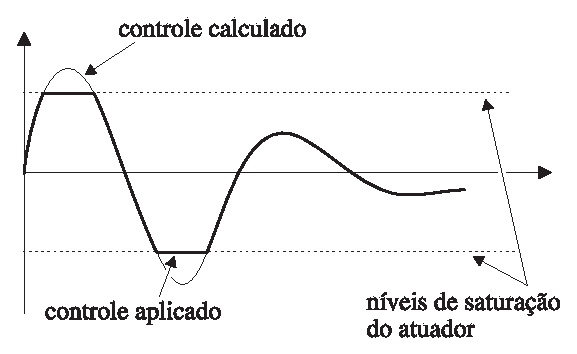
\includegraphics[width=.57\linewidth]{Figuras/sat.eps}
    \caption{Ilustra��o do efeito da satura��o dos atuadores na entrada de controle.}
    \label{fig:sat}
\end{center}\end{figure}

O MPC tem como principal caracter�stica a utiliza��o de um modelo para prever o comportamento do sistema dentro de um determinado {\em horizonte} de tempo futuro. Uma fun��o de custo, v�lida dentro deste horizonte, � minimizada com rela��o a certas vari�veis de decis�o, respeitando-se um conjunto de restri��es impostas. Obt�m-se assim, para cada instante atual, uma seq��ncia de controle �tima com rela��o � fun��o de custo. Embora a predi��o e otimiza��o sejam feitas dentro de toda a extens�o do horizonte, apenas a a��o de controle atual � efetivamente aplicada no sistema. O procedimento � ent�o repetido no pr�ximo instante de tempo, agora com o horizonte de predi��o deslocado um passo adiante e com os estados do sistema atualizados. Obt�m-se assim uma estrat�gia de {\em horizonte deslizante} de controle. 

Para sistemas complexos, multivari�veis e com restri��es, o MPC tornou-se muito bem aceito~\cite{bemporad02}, principalmente na ind�stria de processos onde as plantas a serem controladas s�o suficientemente lentas para permitirem a sua aplica��o~\cite{mayne00}. Originalmente desenvolvido para refinarias de petr�leo e usinas de energia, hoje em dia o MPC j� pode ser encontrado em uma vasta gama de aplica��es, como em ind�strias de alimentos, automotiva, aeroespacial, metalurgia, etc. O interesse no uso do MPC pela ind�stria recai principalmente na capacidade que o mesmo tem de levar em conta as restri��es durante o c�lculo do controle. Assim sendo, a planta � capaz de operar em condi��es mais pr�ximas de seus limites, aumentando a qualidade e a produtividade do processo. Uma extensa revis�o de aplica��es do MPC na ind�stria pode ser vista em~\cite{garcia89,henson98,qin00} e introdu��es te�ricas podem ser vistas em~\cite{allgower99,camacho99}.

Duas grandes vantagens do MPC sobre t�cnicas convencionais de controle ent�o aparecem: a capacidade de considerar restri��es durante o c�lculo da lei de controle e a exist�ncia de um �ndice de desempenho, dado pela minimiza��o de uma fun��o de custo. Por outro lado, o MPC tamb�m apresenta algumas desvantagens. Uma delas � a necessidade de um modelo do sistema para o c�lculo da lei de controle, pois a predi��o dos estados � utilizada no crit�rio de minimiza��o. Assim, uma modelagem imprecisa pode fazer com que o sistema em malha fechada tenha desempenho insatisfat�rio ou at� mesmo causar instabilidade. Outra desvantagem � o alto custo computacional envolvido, j� que um problema de otimiza��o, muitas vezes n�o convexo, com restri��es e de dimens�es elevadas, precisa ser resolvido {\em on-line}. Em sistemas com din�micas r�pidas ou n�o lineares, que � o caso de sistemas eletromec�nicos como os rob�s m�veis, a implementa��o de controladores preditivos permanece essencialmente limitada em sua aplicabilidade, devido ao grande esfor�o computacional necess�rio. Contudo, com o desenvolvimento de computadores de maior capacidade e algoritmos num�ricos mais eficientes, o uso do MPC em tais aplica��es est� se tornando poss�vel.

Assim, a possibilidade de se considerar restri��es durante o c�lculo do controle faz do MPC uma alternativa bastante promissora �s t�cnicas cl�ssicas de controle de rob�s m�veis. Al�m disso, a lei de controle calculada com o MPC � tal que satisfaz as condi��es de Brockett para sistemas n�o holon�micos. Alguns trabalhos envolvendo MPC de rob�s m�veis j� foram desenvolvidos, mas ainda s�o relativamente esparsos. Podem ser citados, por exemplo,~\cite{ollero91,ortega96,yang98,rico99,essen01}. 

Este trabalho tem ent�o como objetivo o estudo da aplicabilidade de algoritmos de MPC, lineares e n�o lineares, para o controle de rob�s m�veis sujeitos a restri��es n�o holon�micas. Dois problemas s�o abordados: estabiliza��o em um ponto e rastreamento de trajet�ria (estabiliza��o ao longo de uma refer�ncia m�vel). Restri��es tanto nas entradas de controle quanto nas vari�veis de estado ser�o consideradas. Resultados de simula��o, desenvolvidos em Matlab, s�o extensivamente mostrados, provando a efic�cia e a aplicabilidade do MPC em rob�s n�o holon�micos.


%%%%%%%%%%%%%%%%%%%%%%%%%%%%%%%%%%
\section{Organiza��o do Documento}
Esta disserta��o est� organizada com segue: 

No Cap�tulo~\ref{cap:wmr} desenvolve-se uma r�pida introdu��o te�rica sobre sistemas sujeitos a restri��es n�o holon�micas. Assim, em seguida � dado o modelo cinem�tico do rob� considerado neste trabalho. O rob� Twil ser� utilizado como estudo de caso (dados construtivos e caracter�sticas f�sicas deste rob� s�o mostrados no Ap�ndice~\ref{app:twil}). Tamb�m s�o mostradas algumas propriedades com rela��o � controlabilidade e estabilizabilidade deste tipo de sistema. Ainda, algumas t�cnicas cl�ssicas de controle, como o controle variante no tempo e o n�o suave, s�o brevemente apresentadas.

O Cap�tulo~\ref{cap:mpc} aborda o m�todo de controle preditivo baseado em modelo. Uma introdu��o ao MPC ser� dada, junto com uma breve perspectiva hist�rica do m�todo. Os algoritmos para a solu��o do MPC nos casos n�o linear e linear s�o dados. No fim deste cap�tulo, � feita uma revis�o sobre alguns trabalhos envolvendo MPC aplicado a rob�s m�veis.

No Cap�tulo~\ref{cap:point}, desenvolve-se a aplica��o do MPC n�o linear ({\em Nonlinear Model-based Predictive Control, NMPC}) para o problema de estabiliza��o do rob� em uma postura fixa. � proposta uma fun��o de custo com as vari�veis de estado em coordenadas polares, e � visto que com esta fun��o de custo o NMPC apresenta uma significativa melhoria de desempenho. Ap�s, restri��es nas vari�veis de estado e nas entradas de controle passam a ser consideradas. Ainda, v�rias compara��es com o NMPC desenvolvido aqui e com t�cnicas cl�ssicas de controle de rob�s n�o holon�micos s�o vistas. Na �ltima se��o deste cap�tulo, um estudo acerca do esfor�o computacional do NMPC para este problema � desenvolvido, a fim de mostrar a aplicabilidade do m�todo em implementa��es reais.

O Cap�tulo~\ref{cap:traj} trata do problema de rastreamento de trajet�ria. Agora, dois m�todos ser�o abordados: um com NMPC e outro que envolve a aplica��o de lineariza��es sucessivas do modelo cinem�tico do rob� ao longo de uma trajet�ria de refer�ncia, sendo poss�vel assim o uso de um MPC linear ({\em Linear Model-based Predictive Control, LMPC}). Um estudo acerca do esfor�o computacional necess�rio para resolver este problema tamb�m � feito. � mostrado que o tempo computacional necess�rio para se resolver o problema de minimiza��o � bastante menor, se comparado ao caso n�o linear, ao mesmo tempo que o desempenho apresentado � bem satisfat�rio.

No Cap�tulo~\ref{cap:conclusions}, ser�o expostas ent�o as conclus�es e algumas sugest�es para trabalhos futuros.

% CAP�TULO 2
\chapter{Rob�s M�veis Dotados de Rodas}\label{cap:wmr}
\section{Introdu��o}
A maioria dos trabalhos existentes na literatura que tratam do controle de rob�s m�veis dotados de rodas sujeitos a restri��es n�o holon�micas utiliza o modelo cinem�tico de um rob� com acionamento diferencial, do tipo {\em uniciclo}. Embora seja uma representa��o bastante simplificada do movimento do ve�culo, o modelo cinem�tico � suficiente para capturar as caracter�sticas n�o holon�micas do sistema.

Como salientado no Cap�tulo~\ref{cap:intro}, o modelo do sistema a ser controlado � um dos elementos essenciais para a aplica��o do MPC. Assim sendo, uma correta modelagem e um perfeito entendimento f�sico do sistema neste ponto � conveniente.

Ent�o, para uma boa compreens�o de como as restri��es n�o holon�micas influenciam no movimento de sistemas mec�nicos como os rob�s m�veis, � dado na primeira se��o deste cap�tulo uma breve descri��o de sistemas sujeitos a restri��es n�o holon�micas. Na seq��ncia, a modelagem cinem�tica baseada no rob� Twil\footnote{Maiores detalhes do rob� Twil s�o descritos no Ap�ndice~\ref{app:twil}.} � desenvolvida, e algumas propriedades de controlabilidade e estabilizabilidade para este sistema s�o apresentadas. Logo ap�s, t�cnicas cl�ssicas de controle de rob�s m�veis baseadas no modelo cinem�tico, como leis variantes no tempo e n�o suaves, s�o brevemente apresentadas.

%%%%%%%%%%%%%%%%%%%%%%%%%%%%%%%%%%%%%%%%%%%%%%%%%%%%%%%%%%%%%%%
\section{Sistemas Mec�nicos N�o Holon�micos}\label{sec:nh_rest}

Em muitos casos, o movimento de sistemas mec�nicos � submetido a certas restri��es que s�o permanentemente satisfeitas durante este movimento, e que tomam a forma de rela��es alg�bricas entre posi��es e velocidades de pontos particulares do sistema~\cite{campion91b}. Considerando um sistema mec�nico de ordem $n$ representado por um vetor $\bf q$ de coordenadas generalizadas e um vetor $\dot{\bf q}$ de velocidades generalizadas,
\begin{equation*}
	\bf q = \begin{bmatrix}
		q_1 \\ q_2 \\ \vdots \\ q_n
	\end{bmatrix}, \qquad
	\dot{\bf q} = \begin{bmatrix}
		\dot q_1 \\ \dot q_2 \\ \vdots \\ \dot q_n
	\end{bmatrix},
\end{equation*}
dois tipos distintos de restri��es podem assim ser observadas~\cite{latombe89,sordalen93a}: 
\begin{itemize}
\item {\bf Restri��es geom�tricas:} s�o representadas por rela��es anal�ticas entre as coordenadas generalizadas $\bf q$ de um sistema mec�nico:
\begin{equation}\label{eqn:rgeom}
	f_i({\bf q})=0, \quad i=1\ldots l
\end{equation}

Quando o sistema � submetido a $l$ restri��es geom�tricas independentes, $l$ coordenadas generalizadas podem ser eliminadas e $n-l$ coordenadas s�o suficientes para fornecer uma total descri��o da configura��o do sistema.

\item{\bf Restri��es cinem�ticas:} S�o representadas por rela��es anal�ticas entre as coordenadas $\bf q$ e as velocidades $\dot{\bf q}$:
\begin{equation*}
	f_i({\bf q},\dot{\bf q})=0, \quad i=1\ldots l
\end{equation*}

Na maioria dos casos, estas restri��es s�o lineares com respeito �s velocidades generalizadas. Ao contr�rio das restri��es geom�tricas, restri��es cinem�ticas n�o necessariamente levam � elimina��o de coordenadas generalizadas da descri��o do sistema. Quando a restri��o � integr�vel, ou {\em holon�mica}, ela pode ser reduzida para a forma da express�o~\req{eqn:rgeom}.

Quando uma restri��o cinem�tica n�o pode ser integrada, esta n�o pode ser usada para eliminar qualquer coordenada generalizada, e diz-se ent�o que esta � uma {\em restri��o n�o holon�mica}, e o sistema que possui estas restri��es � chamado de {\em sistema n�o holon�mico}. Neste caso, o n�mero de graus de liberdade (ou o n�mero de velocidades independentes) � igual ao n�mero de coordenadas generalizadas independentes menos o n�mero de restri��es n�o holon�micas~\cite{neimark72}. A seguir ser�o dados dois exemplos de sistemas com restri��es n�o holon�micas: um disco rolando em um plano e um carro em movimento. Outros exemplos cl�ssicos s�o o plan�metro de A. N. Krylov~\cite{neimark72} e corpos girantes como naves espaciais e ve�culos subaqu�ticos onde a conserva��o do momento angular precisa ser respeitada~\cite{bullo00}.

\end{itemize}

%%%%%%%%%%%%%%%%%%%%%%%%%%%%%%%%%%%%%%%%%%%%%%%%%%%%%%%%%%%%%%%%%%%
\subsection{Exemplo: Um Disco Rolando em um Plano}\label{sec:disco}
Um exemplo cl�ssico de um sistema mec�nico n�o holon�mico � um disco rolando em um plano horizontal~\cite{bloch89,neimark72} percorrendo uma trajet�ria $s$, sem escorregamento ({\em derrapagem}), conforme a Figura~\ref{fig:disco}.

As coordenadas de postura, que descrevem o movimento do disco com rela��o ao plano inercial global $\pi_1$ (espa�o de configura��o) s�o a posi��o, dada pelos eixos $x$ e $y$, e a orienta��o, dada pelo �ngulo $\theta$. $\varphi$ � o �ngulo de rota��o do disco com rela��o ao plano $\pi_2$ (plano de rota��o do disco). Por causa da restri��o de que o disco n�o derrapa, a velocidade no ponto $C$ (ponto de contato do disco com o plano $\pi_1$) � zero. Logo, a magnitude da velocidade tangencial $v$ do centro do disco � proporcional � velocidade angular $\dot{\varphi}$:
\begin{equation*}
	v=r\dot{\varphi},
\end{equation*}	 
onde $r$ � o raio do disco. A dire��o da velocidade � perpendicular ao eixo de rota��o do disco, isto �,
\begin{align*}
	\dot x &= v\cos\theta \\
	\dot y &= v\sin\theta
\end{align*}

Estas condi��es levam �s seguintes restri��es:
\begin{align*}
	\dot x - r\dot\varphi\cos\theta &= 0 \\
	\dot y - r\dot\varphi\sin\theta &= 0
\end{align*}
que n�o podem ser integradas para encontrar uma restri��o holon�mica da forma $f(x,y,\theta,\varphi)=0$. Portanto s�o restri��es {\em n�o holon�micas}.
\begin{figure}[t]\begin{center}
    \includegraphics[width=.8\linewidth]{Figuras/disco.eps}
    \caption{Exemplo cl�ssico de um sistema n�o holon�mico: um disco rolando em um plano.}
    \label{fig:disco}
\end{center}\end{figure}


%%%%%%%%%%%%%%%%%%%%%%%%%%%%%%%%%%%%%%%%%%%%%%%%%%%%%%%%%%
\subsection{Exemplo: Um Carro Estacionando}\label{sec:car}
Um desenho de um carro estacionando � mostrado na Figura \ref{fig:parking} \cite{teel92}. Na aus�ncia de obst�culos, ele pode assumir qualquer configura��o no plano. Logo, o espa�o de configura��o possui tr�s graus de liberdade (dois para a posi��o e um para a orienta��o). Entretanto, assumindo que a componente da velocidade ortogonal ao plano de rota��o $\pi_2$ das rodas � zero (na dire��o de $y'$), a velocidade no ponto central entre duas rodas ativas (o ponto $P$) � sempre tangente � orienta��o do carro (na dire��o de $x'$). Com isso, o espa�o das velocidades, em qualquer configura��o, ter� apenas dois graus de liberdade. Se n�o existissem restri��es ao seu movimento, o caminho tomado para chegar � configura��o final seria, por exemplo, o dado pela linha tracejada. Agora, considerando as restri��es, o carro deve seguir uma trajet�ria semelhante � mostrada pela linha cont�nua. 
\begin{figure}[H]\begin{center}
    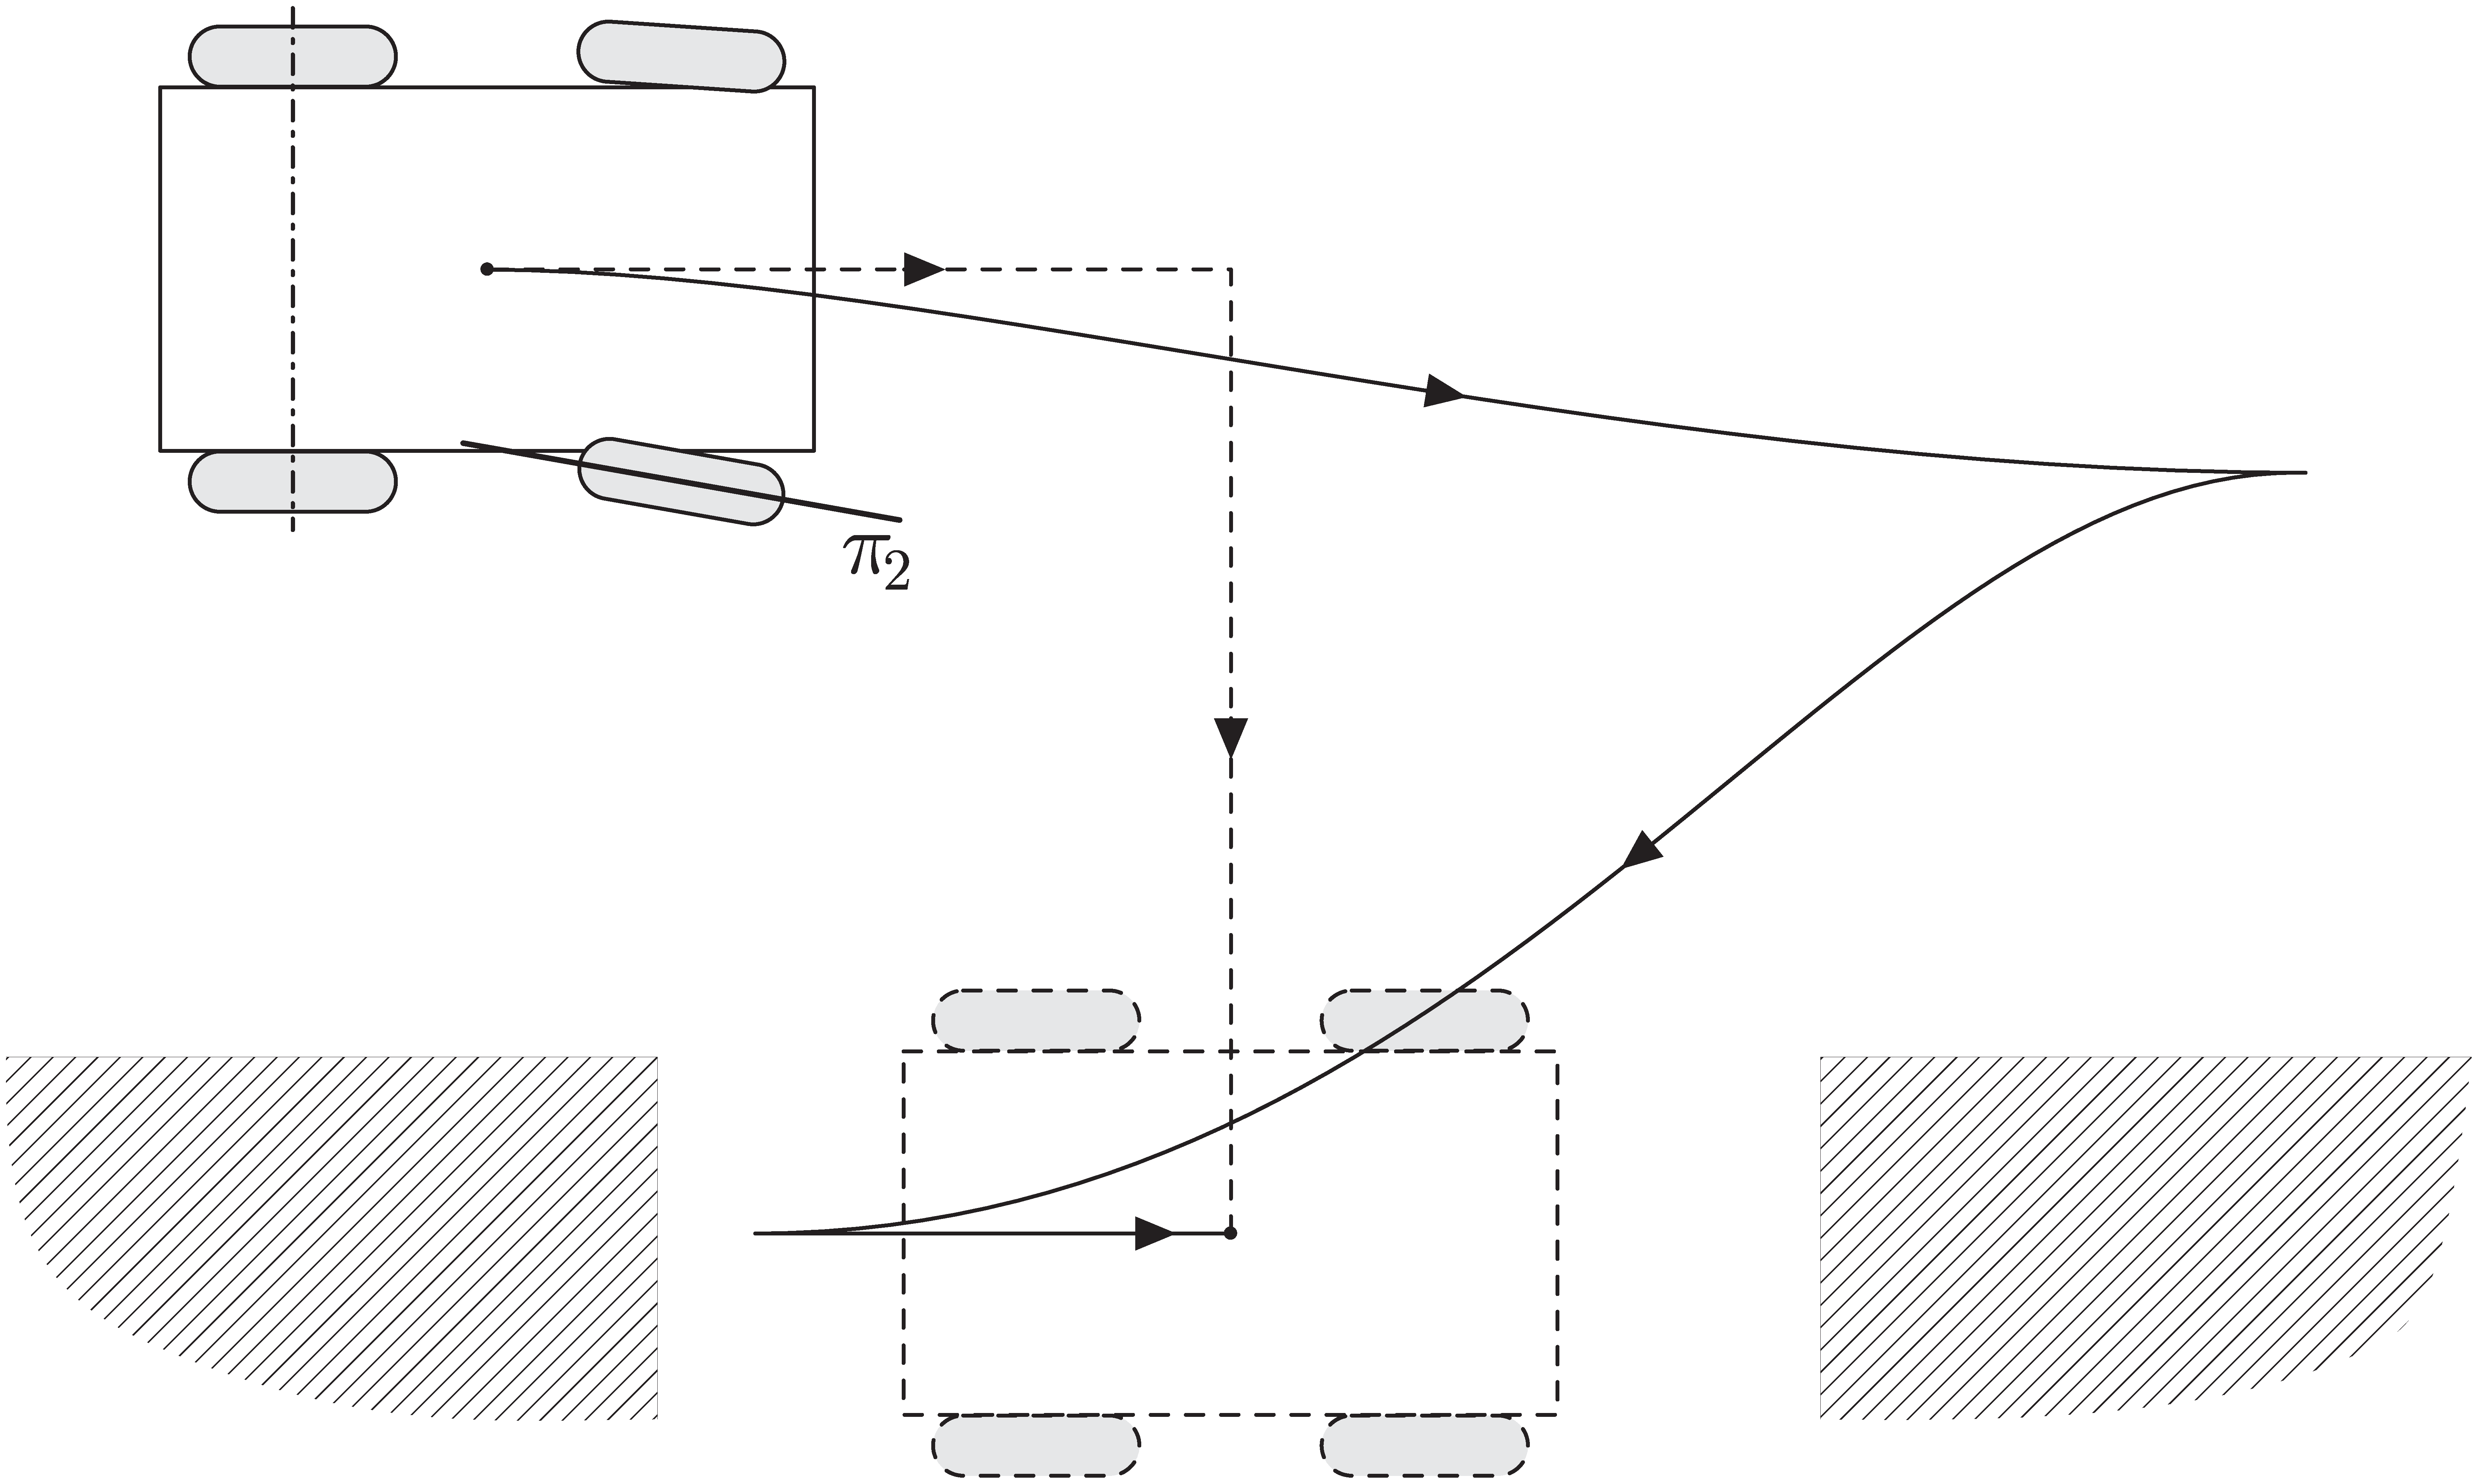
\includegraphics[width=.80\linewidth]{Figuras/parking.eps}
    \caption{Exemplo de trajet�rias para um carro estacionando.}
    \label{fig:parking}
\end{center}\end{figure}

%%%%%%%%%%%%%%%%%%%%%%%%%%%%%%%%%%%%%%%%%%%%%%%%%%%%%%%%%%%%%%%%%%%%%%%%%%%
\section{Cinem�tica de Rob�s M�veis Dotados de Rodas}\label{sec:kinematics}

Para facilitar o entendimento dos resultados apresentados neste e nos pr�ximos cap�tulos, ser� considerado o modelo do rob� m�vel Twil~\cite{lages98a,lages98b} a ser utilizado como estudo de caso neste trabalho. Os dados construtivos do mesmo podem ser vistos com mais detalhes no Ap�ndice~\ref{app:twil}.

Considera-se que o rob� � constitu�do de um corpo r�gido e de rodas n�o deform�veis, e movimenta-se em um plano horizontal. O contato entre as rodas e o plano � puntual. O movimento do rob� � realizado atrav�s de atuadores que fornecem torque para a rota��o das rodas em uma configura��o diferencial. Rob�s m�veis com acionamento diferencial aparecem em grande parte da literatura~\cite{canudas92,indivieri99,lee99,samson91a,fukao00,essen01}. 

Conforme esquematizado na Figura~\ref{fig:robot}, a principal caracter�stica deste tipo de rob� � que o mesmo possui duas rodas fixas centradas (rodas {\em ativas}) que compartilham o mesmo eixo de rota��o, acionadas por dois motores independentes. Uma ou mais rodas orient�veis n�o centrada podem ser usadas a fim de equilibrar o rob�, por isso chamadas de rodas {\em passivas}. Para isto, estas rodas precisam estar localizadas fora do eixo comum �s duas rodas ativas.

Conforme~\cite{campion96}, o {\em modelo cinem�tico de postura} de um rob� com acionamento diferencial tem o seu comportamento descrito pelo seguinte vetor de estados:

\begin{equation*}\label{eqn:states}
	\bf x = \begin{bmatrix}
		x \\ y \\ \theta
	\end{bmatrix},
\end{equation*}	
onde $(x,y)$ e $\theta$ representam, respectivamente, a posi��o e a orienta��o do sistema de coordenadas do rob� $\{C,X_c,Y_c\}$ com rela��o a um sistemas de coordenadas global inercial, $\{O,X,Y\}$. O ponto $C$ na Figura~\ref{fig:robot} � o centro de massa do corpo do rob�, e tamb�m �, neste caso, o centro de rota��o das rodas ativas. 

\begin{figure}[H]\begin{center}
    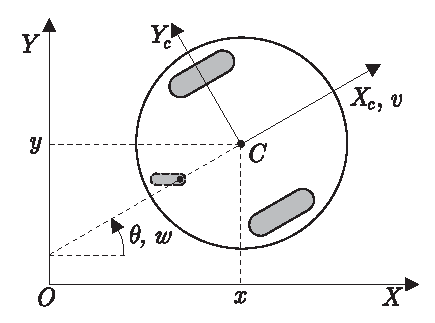
\includegraphics[width=.5\linewidth]{Figuras/robot.eps}
    \caption{Modelo geom�trico de um rob� m�vel com acionamento diferencial.}
    \label{fig:robot}
\end{center}\end{figure}

O modelo cinem�tico � ent�o dado por:
\begin{equation}\label{eqn:model}
	\left\{
		\begin{aligned}
			\dot x	  &= v\cos\theta \\
			\dot y	  &= v\sin\theta \\
			\dot \theta &= w
		\end{aligned}
	\right.
\end{equation}

A entrada de controle � o vetor $\bf u$,
\begin{equation*}
	\bf u = \begin{bmatrix} v \\ w \end{bmatrix},
\end{equation*}	
onde $v$ � a velocidade linear, na dire��o de $X_c$, e $w$ � a velocidade angular.

A seguinte restri��o n�o holon�mica aparece neste caso:
\begin{equation}\label{eqn:nhcond}
	-\dot x\sin\theta + \dot y\cos\theta = 0,
\end{equation}
significando que a velocidade no centro de massa do rob� � ortogonal ao eixo que liga as duas rodas ativas (Figura~\ref{fig:nhcond}).

\begin{figure}[b]\begin{center}
    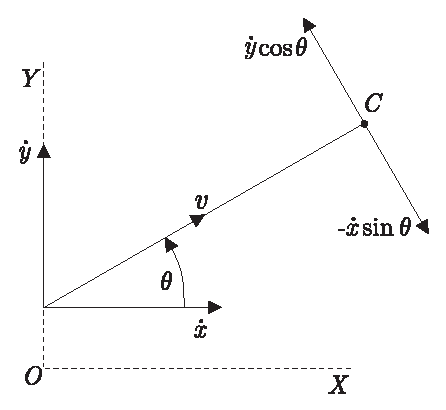
\includegraphics[width=.45\linewidth]{Figuras/nhcond2.eps}
    \caption{A restri��o n�o holon�mica.}
    \label{fig:nhcond}
\end{center}\end{figure}

A express�o~\req{eqn:nhcond} pode ser reescrita da forma
\begin{equation*}
	G({\bf x},\dot{\bf x})=\eta({\bf x})\dot{\bf x} = \sum_{i=1}^{n}\eta_i({\bf x})\dot x_i,
\end{equation*}
onde $n$ � a dimens�o de $\bf x$.

Uma restri��o cinem�tica � holon�mica se, para qualquer $i$, $j$ e $k$ tal que $1\leq i<j<k\leq n$, tem-se ${\cal A}_{ijk}=0$~\cite{latombe89} com:
\begin{equation*}
	{\cal A}_{ijk} = \eta_i\left(\frac{\partial\eta_k}{\partial q_j}-\frac{\partial\eta_j}{\partial q_k}\right) + \eta_j\left(\frac{\partial\eta_i}{\partial q_k}-\frac{\partial\eta_k}{\partial q_i}\right) + \eta_k\left(\frac{\partial\eta_j}{\partial q_i}-\frac{\partial\eta_i}{\partial q_j}\right)
\end{equation*}	

No caso da express�o~\req{eqn:nhcond}, tem-se que o �nico caso � $i=1$, $j=2$ e $k=n=3$, $\eta_1=-\sin\theta$, $\eta_2=\cos\theta$ e $\eta_3=0$ e
\begin{align*}
	{\cal A}_{123} &= -\sin\theta\sin\theta - \cos\theta\cos\theta \\
	               &= -1
\end{align*}
e como ${\cal A}_{123}=-1\neq 0$, conclui-se que a restri��o cinem�tica da express�o~\req{eqn:nhcond} � n�o holon�mica.               


%%%%%%%%%%%%%%%%%%%%%%%%%%%%%%%%%%%%%%%%%%%%%%%%%%%%%%%%%%%%%%%%%%%%%%
\subsection{Propriedades do Modelo Cinem�tico}\label{sec:modelprop}

A express�o~\req{eqn:model} pode ser escrita na seguinte forma compacta:
\begin{equation}\label{eqn:modelshort}
	\dot{\bf x} = f({\bf x}){\bf u},	
\end{equation}
ou, na forma afim:
\begin{equation}\label{eqn:affine}
	\dot{\bf x} = \sum_{i=1}^{m}f_i({\bf x})u_i, \quad {\bf x}\in\real^n, \quad {\bf u}\in\real^m,
\end{equation}
com $n=3$, $m=2$ e
\begin{equation*}
	f_1({\bf x}) = \begin{bmatrix}\cos\theta \\ \sin\theta \\ 0 \end{bmatrix} \qquad
	f_2({\bf x}) = \begin{bmatrix}0 \\ 0 \\ 1 \end{bmatrix}
\end{equation*}	

Embora o modelo cinem�tico da express�o~\req{eqn:model} seja um modelo bastante simplificado do movimento do ve�culo (din�micas dos motores, deforma��es el�sticas e outros efeitos mec�nicos s�o desprezados), o mesmo � suficiente para representar as propriedades n�o holon�micas presentes~\cite{campion96,canudas96}. Ainda, propriedades importantes com rela��o � controlabilidade e estabilizabilidade de rob�s m�veis n�o holon�micos podem ser estabelecidas conforme ser� visto a seguir:

\begin{itemize}
\item {\bf Controlabilidade}.
\begin{definition}
\cite{sontag90}~Um sistema � dito control�vel quando, partindo de uma configura��o inicial, o mesmo pode assumir qualquer configura��o em um intervalo de tempo finito.
\end{definition}

\begin{theorem}\label{teo:cont}
\cite{canudas93}~Uma condi��o suficiente para que um sistema n�o linear descrito pela express�o~\req{eqn:modelshort} seja control�vel � que a dimens�o do fechamento involutivo gerado pelos campos vetoriais $f_1,\ldots,f_m$ seja igual a $n$, $\forall{\bf x}$, i.e.,
\begin{equation*}
	\dim\{\inv\Delta\}=n, \qquad \Delta = {\rm span}\{f_1,\ldots,f_m\}
\end{equation*}
\end{theorem}

Esta condi��o � equivalente, no caso de sistemas lineares, � condi��o de que a matriz de controlabilidade precisa ter posto completo.

A dimens�o de uma distribui��o � dada pelo posto desta distribui��o. Para o sistema da express�o~\req{eqn:affine}, tem-se que $\Delta = {\rm span}\{f_1,f_2\}$ e o fechamento involutivo de $\Delta$ � definido, neste caso, como $\inv\Delta = \{f_1,f_2,[f_1,f_2]\}$ \cite{isidori95} e\footnote{$[f_1,f_2]$ denota o {\em colchete de Lie}, i.e., $[f_1,f_2](x)=\frac{\partial f_2}{\partial x}f_1(x) - \frac{\partial f_1}{\partial x}f_2(x)$.}
\begin{equation*}
	{\rm rank}\{f_1,f_2,[f_1,f_2]\} = {\rm rank}\begin{bmatrix}
		\cos\theta & 0 & \sin\theta \\
		\sin\theta & 0 & -\cos\theta \\
		0 & 1 & 0 \end{bmatrix} = 3,
\end{equation*}

Portanto, a partir do Teorema~\ref{teo:cont}, $\dim\{\inv\Delta\}=3$, de onde conclui-se que o sistema � control�vel.

\item {\bf Lineariza��o}.

Para muitos sistemas n�o lineares, aproxima��es lineares podem ser usadas para uma primeira an�lise na s�ntese da lei de controle. A lineariza��o pode tamb�m fornecer algumas indica��es quanto � controlabilidade e estabilizabilidade do sistema n�o linear. Mais precisamente, se o sistema linearizado � control�vel e estabiliz�vel, ent�o o sistema original n�o linear � control�vel e estabiliz�vel, pelo menos localmente. Entretanto, o inverso n�o pode ser aplicado~\cite{canudas93}. 

No caso do modelo cinem�tico~\req{eqn:model}, a lineariza��o em torno da origem $(\bf x=0, \bf u = 0)$ resulta em
\begin{equation}\label{eqn:linear}
	\dot{\bf x} = \begin{bmatrix}1 & 0 \\ 0 & 0 \\ 0 & 1 \end{bmatrix}
		\begin{bmatrix} v \\ w \end{bmatrix}
\end{equation}

O sistema linear acima � n�o control�vel pois o posto da matriz de controlabilidade
\begin{equation*}
	{\cal C} = \begin{bmatrix} 1 & 0 & 0 & 0 & 0 & 0 \\
						  0 & 0 & 0 & 0 & 0 & 0 \\ 
						  0 & 1 & 0 & 0 & 0 & 0
			 \end{bmatrix}
\end{equation*}	
n�o � completo. Observa-se entretanto que o sistema n�o linear � control�vel, conforme visto pela aplica��o do Teorema~\ref{teo:cont}.

\item {\bf Lineariza��o por realimenta��o de estados}.
\begin{definition}
\cite{khalil96}~Um sistema n�o linear $\dot{\bf x}=f({\bf x},{\bf u})$ � dito lineariz�vel por realimenta��o de estados se existe uma mudan�a de coordenadas
\begin{equation*}
	\xi = T(\bf x)
\end{equation*}
e uma realimenta��o de estados 
\begin{equation*}
	\nu = a({\bf x}){\bf u} + b({\bf x})
\end{equation*}
que transforma o sistema original em um sistema linear.
\end{definition}

Para sistemas sem deriva, tem-se ent�o o seguinte resultado:

\begin{theorem}\label{teo:lin}
\cite{canudas93}~Um sistema da forma~\req{eqn:affine} � localmente lineariz�vel por realimenta��o de estados em torno de $\bf x=0$ se e somente se ${\rm rank}[f_1(0)~~\ldots~~f_m(0)]=n$. 
\end{theorem}

Para o caso do modelo cinem�tico da express�o~\req{eqn:affine}, tem-se que
\begin{equation*}
	{\rm rank}\left[f_1(0)~~f_2(0)\right] = 
	{\rm rank}\begin{bmatrix}
		1 & 0 \\ 0 & 0 \\ 0 & 1
	\end{bmatrix} < n
\end{equation*}
e a lineariza��o de todos os estados do sistema n�o linear n�o � poss�vel. Esta condi��o � equivalente � condi��o de controlabilidade do sistema linearizado~\req{eqn:linear}, que tamb�m n�o � satisfeita. Ainda assim, � poss�vel linearizar parte dos estados, como por exemplo a posi��o apenas~\cite{kuhne04a}. Muitas vezes isto n�o � muito restritivo, se o rob� possui uma geometria circular e o objetivo � estabilizar apenas a posi��o, descartando a orienta��o do rob�.

\item {\bf Estabiliza��o atrav�s de realimenta��o est�tica e suave}.

O problema da estabiliza��o atrav�s de uma lei de controle est�tica e suave pode ser formulado como encontrar um controle ${\bf u}=k({\bf x})$, com $k({\bf x})$ est�tica e suave, tal que o sistema em malha fechada $\dot{\bf x}=f({\bf x})k({\bf x})$ seja assintoticamente est�vel. Pode-se ent�o enunciar o seguinte resultado a respeito das condi��es estudadas por Brockett:
\begin{theorem}\label{teo:brockett}
\cite{brockett82}~Considerando novamente o sistema da express�o~\req{eqn:affine}, com $m\leq n$. Se os campos vetoriais $f_i(0)$, $i=1,\ldots,m$ s�o linearmente independentes, i.e.,
\begin{equation*}
	{\rm rank}[f_1(0)~~f_2(0)~~\cdots~~f_m(0)] = m,
\end{equation*}
ent�o existe uma lei de controle est�tica e suave do tipo ${\bf u}=k({\bf x})$ que estabiliza o sistema~\req{eqn:affine} se e somente se $m=n$.
\end{theorem}

Para o modelo cinem�tico da express�o~\req{eqn:model}, tem-se que $n=3$, $m=2$ e
\begin{equation*}
	f_1(0) = \begin{bmatrix} 1 \\ 0 \\ 0 \end{bmatrix} \qquad
	f_2(0) = \begin{bmatrix} 0 \\ 0 \\ 1 \end{bmatrix}
\end{equation*}

Assim, ${\rm rank}[f_1(0)~~f_2(0)]=2$ e n�o existe lei de controle est�tica e suave ${\bf u}=k({\bf x})$ para o sistema considerado. De fato, diferentemente dos sistemas lineares, a controlabilidade de um sistema n�o linear n�o implica na exist�ncia de leis suaves est�ticas estabilizantes. O Teorema~\ref{teo:brockett} corresponde a uma particulariza��o das condi��es de Brockett~\cite{brockett82} para o caso de sistemas sem deriva.


\end{itemize}

%%%%%%%%%%%%%%%%%%%%%%%%%%%%%%%%%%%%%%%%%%%%%%%%%%%%%%%%%%%%%%%%%%%%%%%%%%%%%%%%%%%%%%%%
\section{M�todos Cl�ssicos Para o Controle de Rob�s M�veis}\label{sec:classical_control}

O controle de sistemas mec�nicos n�o holon�micos, como os rob�s m�veis, tem sido objeto de um grande esfor�o de pesquisa da comunidade cient�fica nos �ltimos anos. A raz�o para isto se d� basicamente pelo seguinte~\cite{aguiar00}:
\begin{itemize}
\item existe um grande n�mero de rob�s, nas mais variadas aplica��es, que possuem restri��es n�o holon�micas;
\item h� um consider�vel desafio na s�ntese de leis de controle para sistemas n�o lineares que n�o podem ser transformados em sistemas lineares; 
\item conforme Brockett~\cite{brockett82}, um sistema com restri��es n�o holon�micas n�o pode ser estabilizado em um ponto de equil�brio, por uma lei de controle suave e invariante no tempo.
\end{itemize}

Quanto ao objetivo, pode-se classificar as metodologias de controle em malha fechada para rob�s m�veis em basicamente tr�s tipos:
\begin{itemize}
\item {\em Estabiliza��o em um ponto.} Para um sistema linear invariante no tempo, se os autovalores inst�veis s�o control�veis (i. e., se o sistema � estabiliz�vel), um ponto de equil�brio pode ser assintoticamente estabilizado por uma realimenta��o de estados est�tica, suave e invariante no tempo. Entretanto, para sistemas n�o lineares e com restri��es n�o holon�micas, isto n�o � mais poss�vel~\cite{brockett82}. Conseq�entemente, ferramentas lineares antes utilizadas n�o podem mais ser consideradas, nem localmente \cite{kolmanovsky95}, conforme mostrado nos Teoremas~\ref{teo:cont}-\ref{teo:brockett}. Neste caso, usualmente, leis de controle variantes no tempo ou n�o suaves s�o utilizadas a fim de transpor as restri��es de Brockett, como ser� estudado nas Se��es~\ref{sec:timevar}, \ref{sec:disc} e no Cap�tulo~\ref{cap:point}.

Al�m do controle variante no tempo e do controle n�o suave, outros m�todos incluem ainda controle h�brido (combina��o dos dois m�todos)~\cite{pomet92,canudas94,canudas95}, controle adaptativo (considera incertezas do modelo)~\cite{lee99,fukao00,oya03} e lineariza��o por realimenta��o din�mica de estados~\cite{dong01,oriolo02,sun05}. O interesse por esta �ltima t�cnica baseia-se no fato de que, se a lineariza��o do sistema existe, leis de controle lineares podem ser obtidas. Ainda, � poss�vel obter-se uma descri��o linear mais representativa do sistema n�o linear, ao contr�rio do obtido por expans�o em s�ries de Taylor~\cite{lages98a,chaves00}.

\item {\em Rastreamento de trajet�ria.} A fim de superar as limita��es impostas pelo Teorema de Brockett, v�rias abordagens diferentes foram propostas. Alguns m�todos abandonam a id�ia da estabiliza��o em um ponto e procuram obter converg�ncia a uma trajet�ria de refer�ncia, parametrizada no tempo. Neste caso, o problema � resolvido em duas etapas distintas: primeiro uma trajet�ria � calculada {\em off-line} e em seguida uma lei de controle � projetada a fim de fazer com que o rob� siga a tajet�ria calculada anteriormente. Usualmente, a exist�ncia de um rob� de refer�ncia virtual � considerada, descrito, por exemplo, pelo modelo cinem�tico $\dot{\bf x}_r=f({\bf x}_r,{\bf u}_r)$. Assume-se ent�o que, para entradas de refer�ncia n�o nulas, deseja-se calcular uma lei de controle que fa�a que o erro entre o rob� e a refer�ncia seja nula. Trabalhos neste sentido encontram-se em~\cite{yamamoto94,pomet92,kanayama90,campion91a,deng93,yang99,do02,sun05}. Este caso ser� tratado com mais detalhes no Cap�tulo~\ref{cap:traj}.

\item {\em Seguimento de caminho.} Neste caso, � semelhan�a do caso acima, tamb�m deseja-se que o rob� convirga para uma trajet�ria de refer�ncia, mas geralmente, este problema � menos restritivo, pois n�o h� especifica��o temporal para que esta converg�ncia seja alcan�ada. Ainda, usualmente considera-se que a velocidade linear � mantida constante e a converg�ncia � obtida apenas atrav�s da velocidade angular. Trabalhos utilizando seguimento de caminho s�o encontrados em~\cite{samson95,sarkar93,encarnacao02}. Este problema n�o ser� estudado neste trabalho.
\end{itemize}

A seguir ser�o apresentadas algumas t�cnicas existentes na literatura que foram escolhidas de forma a representar e abranger concisamente os trabalhos j� desenvolvidos na �rea de controle de rob�s m�veis n�o holon�micos.


%%%%%%%%%%%%%%%%%%%%%%%%%%%%%%%%%%%%%%%%%%%%%%%%%%%%%%%%%%
\subsection{Controle Variante no Tempo}\label{sec:timevar}

Leis de controle variantes no tempo utilizadas em sistemas n�o holon�micos foram estudadas primeiramente por~\cite{samson90}. Nesta refer�ncia, o controle utilizado era, em sua vers�o mais simples, da forma:
\begin{align*}
	v &= -k_1x \\
	w &= -g(t)y - k_3\theta
\end{align*}
sendo $v$ e $w$ as entradas de controle. $k_1$ e $k_3$ s�o constantes reais positivas e $g(t)$ � escolhida tal que $\frac{\partial g}{\partial t}(t)$ n�o tende a zero quando o tempo $t$ tende ao infinito. Por exemplo, $g(t)=\sin(t)$. Leis de controle variantes no tempo possuem a desvantagem de apresentar baixas taxas de converg�ncia e trajet�rias altamente oscilat�rias~\cite{gurvits93,campion96}, o que, em uma implementa��o real, pode se tornar at� n�o fact�vel, dependendo das amplitudes e taxas de varia��o das entradas de controle. Outros trabalhos que utilizam controle variante no tempo podem ser citados:~\cite{teel92,tarin99,murray97,dixon99,do02}.

Tr�s exemplos de leis de controle variantes no tempo existentes na literatura ser�o apresentadas aqui. Todas elas utilizam o sistema
\begin{equation}\label{eqn:model2}
	\left\{
		\begin{aligned}
			\dot x	  &= v\cos\theta \\
			\dot y	  &= v\sin\theta \\
			\dot \theta &= w
		\end{aligned}
	\right.
\end{equation}
onde $[x~~y~~\theta]^T$ representa a configura��o	do rob� com rela��o ao espa�o de configura��o e $[v~~w]^T$ s�o as velocidades linear e angular, respectivamente, conforme o modelo cinem�tico~\req{eqn:model2}. O objetivo � estabilizar o rob� em uma postura fixa que, sem perda de generalidade, � a origem: $x=0$, $y=0$, $\theta=0$.

%%%%%%%%%%%%%%%%%%%%%%%%%%%%%%%%%%%%%%%%%%%%%%%
\subsubsection{\cite{pomet92}}\label{sec:pomet}
Neste trabalho a seguinte lei de controle � utilizada:
\begin{align*}
	v = &-x\cos\theta-y\sin\theta \\
	w = &-a\cos\frac{\theta}{a}\sin\frac{\theta}{a} + \\ &+ a\lambda\cos^2\frac{\theta}{a}\bigl(-y(\sin t-\cos t)-y\sin\theta+x\cos\theta)\cos t\sin\theta\bigr),
\end{align*}
onde $t$ � o tempo e $a$ e $\lambda$ s�o n�meros reais positivos, com $a>2$. A fun��o de Lyapunov utilizada para provar a estabilidade desta lei de controle � a seguinte:
\begin{equation*}
	V = \frac{1}{2}x^2+\frac{1}{2}y^2+\frac{1}{2}\left(\tan\frac{\theta}{a}\lambda+x\cos t\right)^2
\end{equation*}

Os resultados s�o mostrados abaixo, para uma condi��o inicial ${\bf x}_0=[x_0~~y_0~~\theta_0]^T=[2~~2~~\pi]^T$ (identificada, no plano $XY$, pelo s�mbolo $\odot$\footnote{Durante todo este trabalho, nos gr�ficos da trajet�ria no plano $XY$, a posi��o inicial do rob� � indicada por $\odot$, a posi��o final por $\times$ e a origem por $+$.}) e constantes $a=4$ e $\lambda=2,1$.
\begin{figure}[H]\begin{center}
    \includegraphics[width=.6\linewidth]{Figuras/pomet/traj_01.eps}
    \caption{Trajet�ria no plano $XY$. Controle de~\cite{pomet92}.}
    \label{fig:pomet_traj_01}
\end{center}\end{figure}
\begin{figure}[H]\begin{center}
    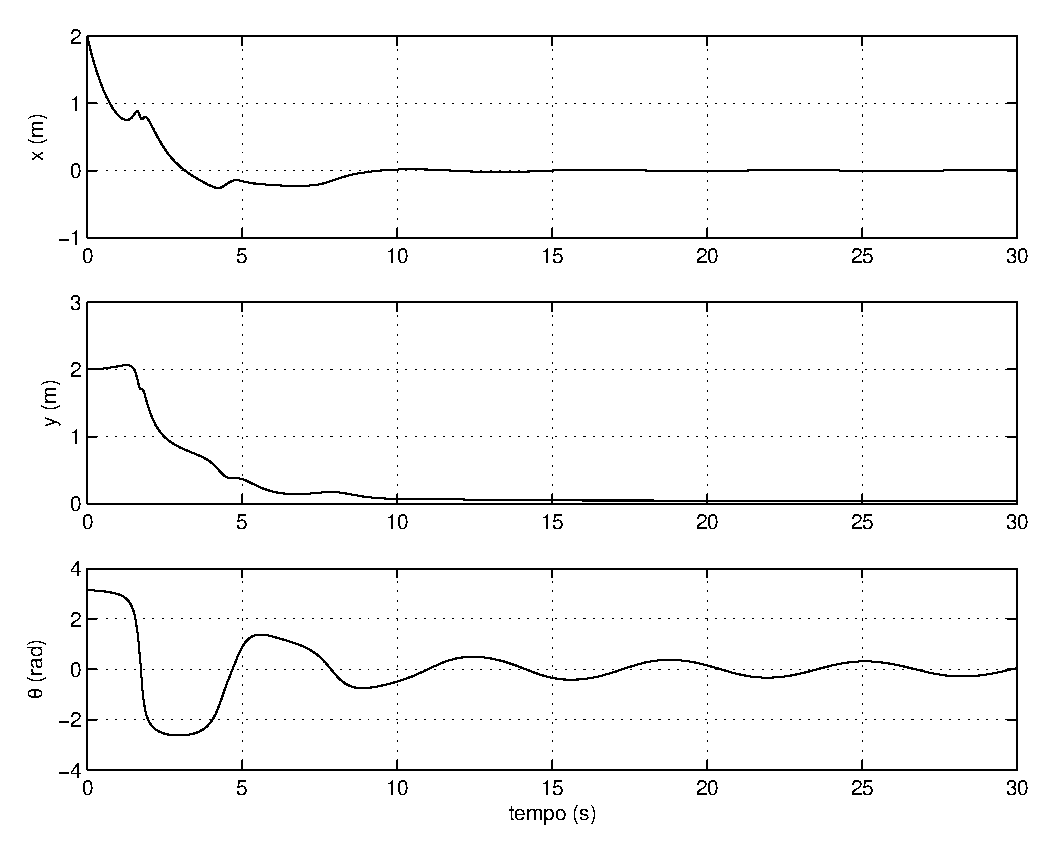
\includegraphics[width=.6\linewidth]{Figuras/pomet/state_01.eps}
    \caption{Estados $x$, $y$ e $\theta$. Controle de~\cite{pomet92}.}
    \label{fig:pomet_state_01}
\end{center}\end{figure}
\begin{figure}\begin{center}
    \includegraphics[width=.6\linewidth]{Figuras/pomet/control_01.eps}
    \caption{Entradas de controle $v$ e $w$. Controle de~\cite{pomet92}.}
    \label{fig:pomet_control_01}
\end{center}\end{figure}

Na Figura~\ref{fig:pomet_traj_01} � mostrada a trajet�ria que o rob� percorre no plano de configura��o $XY$. Os estados e as entradas de controle s�o mostrados individualmente ao longo do tempo nas Figuras~\ref{fig:pomet_state_01} e~\ref{fig:pomet_control_01}, respectivamente. Observa-se um comportamento altamente oscilat�rio e um tempo de acomoda��o elevado, caracter�sticas de leis variantes no tempo. Ainda, as amplitudes das entradas de controle, se consideradas as caracter�sticas do rob� Twil (Ap�ndice~\ref{app:twil}) tornam esta lei de controle proibitiva do ponto de vista pr�tico. Os limites das velocidades linear e angular s�o de, respectivamente, $0,4712~m/s$ e $3,7699~rad/s$, valores estes que s�o largamente ultrapassados, como observa-se na Figura~\ref{fig:pomet_control_01}. Talvez a sintonia dos par�metros $a$ e $\lambda$ pode fazer com que as amplitudes das entradas de controle sejam menores. Entretanto, n�o existe um m�todo sistem�tico para escolher estes par�metros de forma a melhorar o desempenho ou de levar em conta restri��es nos estados ou nas entradas de controle. Os valores utilizados neste caso foram obtidos atrav�s da an�lise de diversos casos, chegando-se ent�o a uma solu��o aceit�vel, para este caso, com rela��o �s trajet�rias de estado.


%%%%%%%%%%%%%%%%%%%%%%%%%%%%%%%%%%%%%%%%%%%%%%%%%%
\subsubsection{\cite{samson91b}}\label{sec:samson}
Este trabalho apresenta uma lei de controle que estabiliza o sistema~\req{eqn:model2}
assintoticamente. Fazendo uma transforma��o de coordenadas da base cartesiana $(x,y,\theta)$ para uma base variante no tempo $(z_1,z_2,z_3)$
\begin{align*}
	z_1 &= x\cos\theta+y\sin\theta \\
	z_2 &= -x\sin\theta+y\cos\theta \\
	z_3 &= \theta + f(z_2,t)
\end{align*}
tem-se que
\begin{equation}\label{eqn:model3}
	\begin{aligned}
		\dot z_1 &= v + z_2w \\
		\dot z_2 &= -z_1w \\
		\dot z_3 &= w - z_1w\frac{\partial f}{\partial z_2}+\frac{\partial f}{\partial t}
	\end{aligned}		
\end{equation}

Escolhendo $f(z_2,t)=z_2\sin t$, $\frac{\partial f}{\partial z_2}=\sin t$, $\frac{\partial f}{\partial t}=z_2\cos t$ e a seguinte lei de controle resulta em estabiliza��o assint�tica para o sistema~\req{eqn:model3}:
\begin{align*}
	w &= -z_3 - \frac{\partial f}{\partial t} = -z_3 - z_2\cos t \\
	v &= -z_1 + z_3w\frac{\partial f}{\partial z_2} = -z_1 + z_3w\sin t
\end{align*}

E os resultados s�o mostrados abaixo, para uma condi��o inicial ${\bf x}_0=[-2,5~~1,3~~\pi/2]^T$.
\begin{figure}[H]\begin{center}
    \includegraphics[width=.6\linewidth]{Figuras/samson/traj_01.eps}
    \caption{Trajet�ria no plano $XY$. Controle de~\cite{samson91b}.}
    \label{fig:samson_traj_01}
\end{center}\end{figure}
\begin{figure}[H]\begin{center}
    \includegraphics[width=.6\linewidth]{Figuras/samson/state_01.eps}
    \caption{Estados $x$, $y$ e $\theta$. Controle de~\cite{samson91b}.}
    \label{fig:samson_state_01}
\end{center}\end{figure}
\begin{figure}\begin{center}
    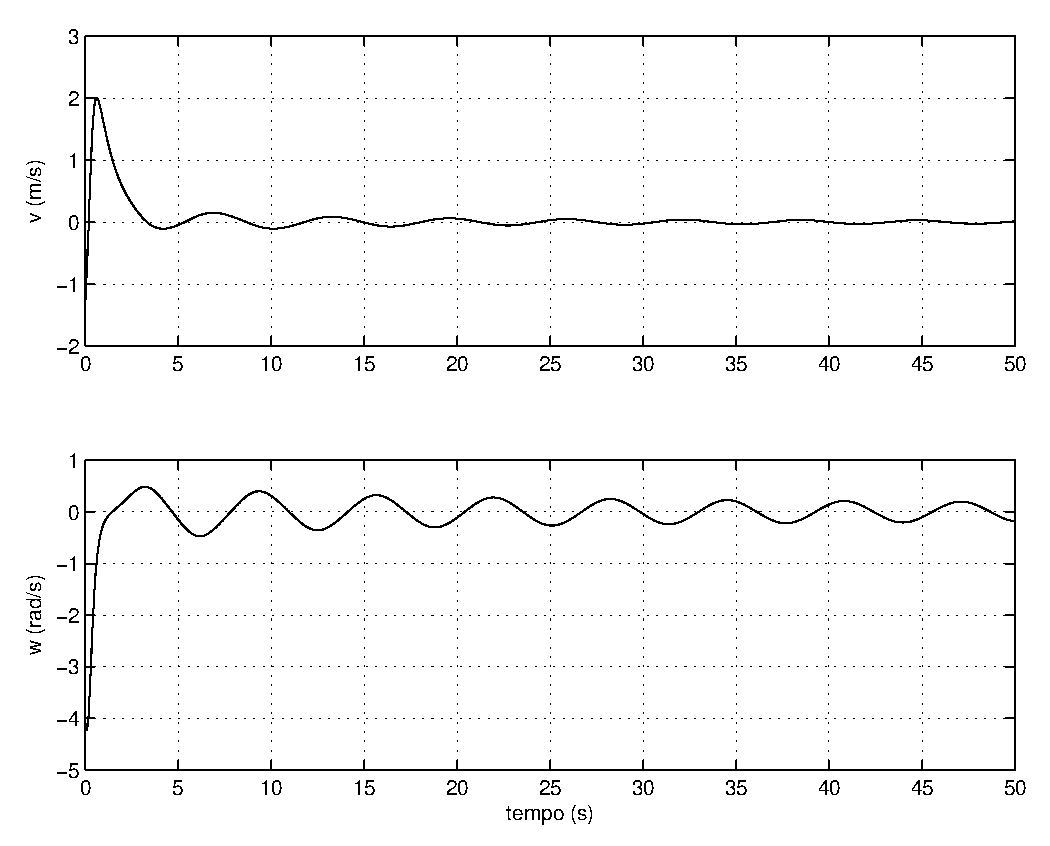
\includegraphics[width=.6\linewidth]{Figuras/samson/control_01.eps}
    \caption{Entradas de controle $v$ e $w$. Controle de~\cite{samson91b}.}
    \label{fig:samson_control_01}
\end{center}\end{figure}

A exemplo da lei de controle anterior, observa-se um movimento altamente oscilat�rio e um tempo de acomoda��o elevado. Da Figura~\ref{fig:samson_control_01}, nota-se que os limites de amplitude das entradas de controle foram tamb�m ultrapassados. Talvez com outra escolha para a fun��o $f(z_2,t)$, estes problemas possam ser minimizados.

%%%%%%%%%%%%%%%%%%%%%%%%%%%%%%%%%%%%%%%%%%%%%
\subsubsection{\cite{teel95}}\label{sec:teel}
Este trabalho utiliza uma transforma��o can�nica do sistema para a forma encadeada. Trabalhos envolvendo controle de sistemas n�o holon�micos na forma encadeada s�o vistos em \cite{bloch89,murray90,teel92,canudas94,wu99}. A vantagem � que a lei de controle pode ser facilmente generalizada para v�rios tipos de sistemas n�o holon�micos~\cite{bloch89,murray93,sordalen93b}. Assim, fazendo
\begin{align*}
	z_1 &= \theta \\
	z_2 &= x\cos\theta+y\sin\theta \\
	z_3 &= x\sin\theta-y\cos\theta
\end{align*}
e
\begin{align*}
	u_1 &= w \\
	u_2 &= v - z_3w,
\end{align*}
tem-se que o sistema do modelo cinem�tico � transformado para a seguinte forma encadeada:
\begin{align*}
	\dot z_1 &= u_1 \\
	\dot z_2 &= u_2 \\
	\dot z_3 &= z_2u_1
\end{align*}
que � estabilizado atrav�s da seguinte lei de controle:
\begin{align*}
	u_1 &= -z_1 + z_3\cos t \\
	u_2 &= -z_2 + z_3^2\sin t
\end{align*}

A seguinte fun��o de Lyapunov garante estabilidade para a lei de controle acima:
\begin{equation*}
	V = \left(z_1-\frac{z_3}{2}(\cos t+\sin t)\right)^2 + \left(z_2-\frac{z^2_3}{2}(\sin t-\cos t)\right)^2 + z^2_3
\end{equation*}	

E os resultados s�o mostrados abaixo, para uma condi��o inicial ${\bf x}_0=[0~~-3,2~~\pi/4]^T$.
\begin{figure}[H]\begin{center}
    \includegraphics[width=.6\linewidth]{Figuras/murray/traj_01.eps}
    \caption{Trajet�ria no plano $XY$. Controle de~\cite{teel95}.}
    \label{fig:murray_traj_01}
\end{center}\end{figure}
\begin{figure}[H]\begin{center}
    \includegraphics[width=.6\linewidth]{Figuras/murray/state_01.eps}
    \caption{Estados $x$, $y$ e $\theta$. Controle de~\cite{teel95}.}
    \label{fig:murray_state_01}
\end{center}\end{figure}
\begin{figure}\begin{center}
    \includegraphics[width=.6\linewidth]{Figuras/murray/control_01.eps}
    \caption{Entradas de controle $v$ e $w$. Controle de~\cite{teel95}.}
    \label{fig:murray_control_01}
\end{center}\end{figure}

Novamente as caracter�sticas das leis de controle variantes no tempo s�o observadas: trajet�rias de estado altamente oscilat�rias e um elevado tempo de acomoda��o. Nota-se tamb�m que o limite aceit�vel da velocidade linear, para o rob� Twil, � ultrapassado.


%%%%%%%%%%%%%%%%%%%%%%%%%%%%%%%%%%%%%%%%%%%%%%%
\subsection{Controle N�o Suave}\label{sec:disc}

As leis de controle n�o suaves podem ser subdivididas em leis cont�nuas por partes ou de modo deslizante. A vantagem do controle n�o suave � que o mesmo pode superar as desvantagens comumente associadas ao controle variante no tempo, ou seja, baixa taxa de converg�ncia e trajet�rias de estado oscilat�rias. O trabalho pioneiro nesta t�cnica foi~\cite{bloch89}. Trabalhos subseq�entes s�o encontrados em~\cite{bloch92,canudas92,chacal94,su94}. Como ser� visto, apesar de resolver os problemas apresentados pelas leis variantes no tempo, ainda n�o � poss�vel com leis de controle descont�nuas incluir restri��es nos estados ou nas entradas de controle.

A exemplo da se��o anterior, ser�o mostrados agora leis de controle n�o suaves existentes na literatura para o problema de estabiliza��o do rob� em um ponto.

%%%%%%%%%%%%%%%%%%%%%%%%%%%%%%%%%%%%%%%%%%%%%%%%
\subsubsection{\cite{lages98a}}\label{sec:lages}
Neste trabalho e tamb�m em \cite{astolfi94,lages98b,indivieri99,chwa04}, o modelo cinem�tico~\req{eqn:model2} � transformado em coordenadas polares atrav�s da seguinte transforma��o descont�nua\footnote{A fun��o $\atan(y,x)$ calcula o valor do arco tangente de $y/x$, usando os sinais dos dois argumentos para determinar o quadrante do valor retornado.}, conforme a Figura~\ref{fig:polar2}:
\begin{align*}
	e      &= \sqrt{x^2+y^2} \\
	\phi   &= \atan(y,x) \\
	\alpha &= \theta-\phi
\end{align*}

\begin{figure}[htbp]\begin{center}
    \includegraphics[width=.45\linewidth]{Figuras/polar.eps}
    \caption{Coordenadas polares para o rob� com acionamento diferencial.}
    \label{fig:polar2}
\end{center}\end{figure}

Assim, o seguinte modelo cinem�tico � obtido:
\begin{equation*}
	\left\{
		\begin{aligned}
			\dot e	  &= v\cos\alpha \\
			\dot \phi	  &= v\frac{\sin\alpha}{e} \\
			\dot \alpha &= -v\frac{\sin\alpha}{e}+w
		\end{aligned}
	\right.
\end{equation*}

Este sistema � n�o definido quando $e=0$. Assim, o sistema na base polar de coordenadas torna-se descont�nuo, sendo poss�vel assim transpor as condi��es de Brockett e estabilizar o sistema acima na origem atrav�s de uma lei de controle suave e invariante no tempo. Ent�o, atrav�s da seguinte fun��o de Lyapunov:
\begin{equation*}
	V = \frac{1}{2}\left(\lambda e^2+h\phi^2+\alpha^2\right),
\end{equation*}
chega-se ao seguinte controle:
\begin{align*}
	v &= -\gamma_1e\cos\alpha \\
	w &= -\gamma_2\alpha-\gamma_1\cos\alpha\frac{\sin\alpha}{\alpha}\left(\alpha-h\phi\right)
\end{align*}
onde $\lambda$, $h$, $\gamma_1$ e $\gamma_2$ s�o constantes reais positivas. Esta lei de controle, quando transformada para base original de coordenadas cartesianas, torna-se descont�nua~\cite{lages98a}. Os resultados s�o mostrados abaixo, para uma condi��o inicial de ${\bf x}_0=[-0,2~~3~~0]^T$ e $\gamma_1=0,05$, $\gamma_2=0,1$ e $h=1,35$.

\begin{figure}[H]\begin{center}
    \includegraphics[width=.6\linewidth]{Figuras/lages/traj_01.eps}
    \caption{Trajet�ria no plano $XY$. Controle de~\cite{lages98a}.}
    \label{fig:lages_traj_01}
\end{center}\end{figure}
\begin{figure}[H]\begin{center}
    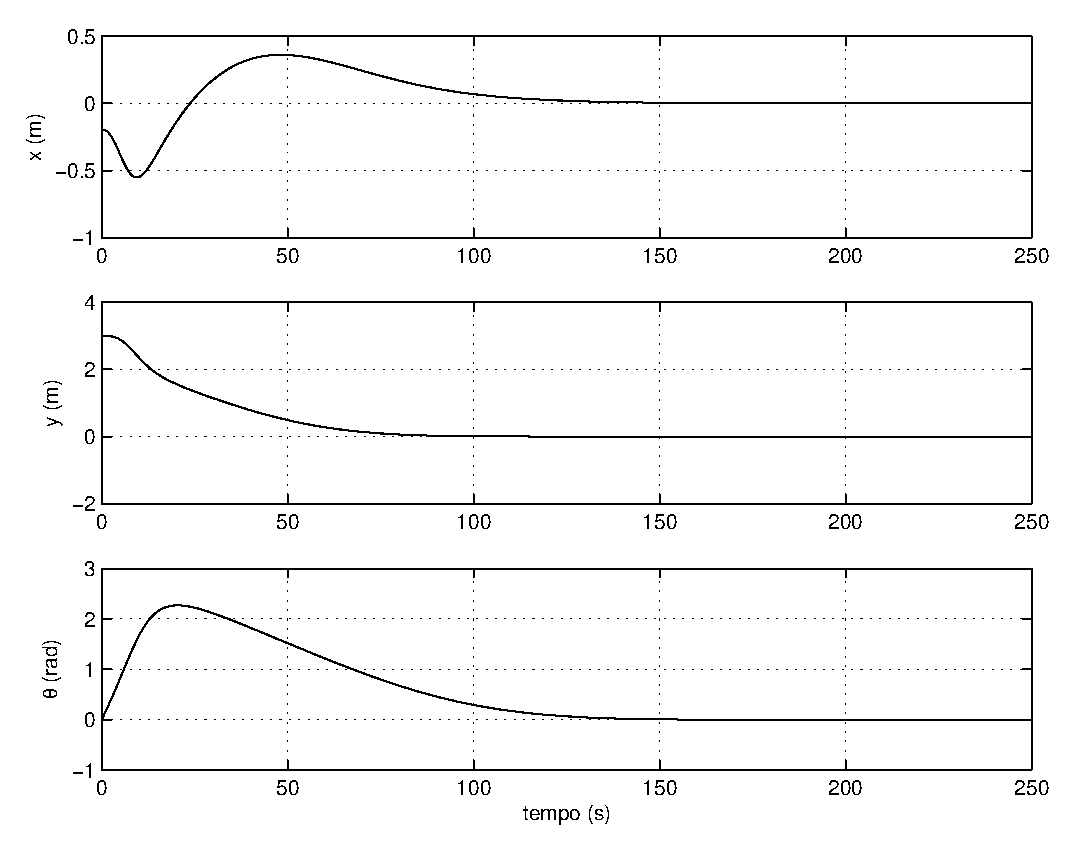
\includegraphics[width=.6\linewidth]{Figuras/lages/state_01.eps}
    \caption{Estados $x$, $y$ e $\theta$. Controle de~\cite{lages98a}.}
    \label{fig:lages_state_01}
\end{center}\end{figure}
\begin{figure}[H]\begin{center}
    \includegraphics[width=.6\linewidth]{Figuras/lages/control_01.eps}
    \caption{Entradas de controle $v$ e $w$. Controle de~\cite{lages98a}.}
    \label{fig:lages_control_01}
\end{center}\end{figure}

Nota-se aqui uma lei de controle que gera uma trajet�ria de estado bastante suave, como observa-se pelas figura~\ref{fig:lages_traj_01} e \ref{fig:lages_state_01}. Ainda, as amplitudes das entradas de controle (Figura~\ref{fig:lages_control_01}) s�o compat�veis com os limites definidos para o rob� Twil. � claro que, com isso, o tempo com que o rob� chega na origem � maior. Com a sintonia dos par�metros existentes para esta lei de controle ($h$, $\gamma_1$ e $\gamma_2$), a taxa de converg�ncia pode ser aumentada, diminuindo assim o tempo de acomoda��o. Entretanto, n�o existe m�todo sistem�tico para isto e a modifica��o destes par�metros pode gerar entradas de controle com amplitudes elevadas. A condi��o final do rob� � ${\bf x}_f=[0~~0~~0]^T$.

%%%%%%%%%%%%%%%%%%%%%%%%%%%%%%%%%%%%%%%%%%%%%%%%%%%%%%
\subsubsection{\cite{sordalen93a}}\label{sec:sordalen}
Este m�todo tamb�m utiliza uma transforma��o descont�nua de coordenadas (Figura~\ref{fig:sordalen}). 
\begin{figure}[H]\begin{center}
    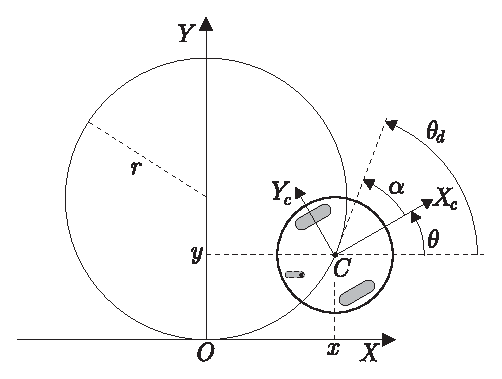
\includegraphics[width=.54\linewidth]{Figuras/sordalen.eps}
    \caption{Transforma��o descont�nua de coordenadas.}
    \label{fig:sordalen}
\end{center}\end{figure}

Assim, define-se:
\begin{align*}
	a &= r\theta_d \\
	\alpha &= e - 2\pi n(e)
\end{align*}
onde
\begin{align*}
	r &= \frac{x^2+y^2}{2y} \\
	\theta_d &= \begin{cases}
		2\atan(y,x) & ;~(x,y)\neq(0,0) \\
		0           & ;~(x,y)=(0,0)
	\end{cases} \\
	e &= \theta-\theta_d
\end{align*}
e $n(e)\in\{0,\pm1,\pm2,\ldots\}$ � uma fun��o que faz com que $\alpha\in[-\pi,\pi)$. A seguinte lei de controle estabiliza o rob� na origem exponencialmente:
\begin{align*}
	v &= -\gamma b_1a \\
	w &= -b_2v - k\alpha
\end{align*}
onde $\gamma$ e $k$ s�o constantes reais positivas e
\begin{align*}
	b_1 &= \cos\theta\left(\frac{\theta_d}{\beta}-1\right) + \sin\theta\left(\frac{\theta_d}{2}\left(1-\frac{1}{\beta^2}\right)+\frac{1}{\beta}\right) \\
	b_2 &= \frac{2}{(1+\beta^2)x}\left(\beta\cos\theta-\sin\theta\right)
\end{align*}
com $\beta= y/x$.

Assim, os seguintes resultados s�o obtidos, para uma condi��o final de ${\bf x}_0=[-0,2~~3~~0]^T$.
\begin{figure}[H]\begin{center}
    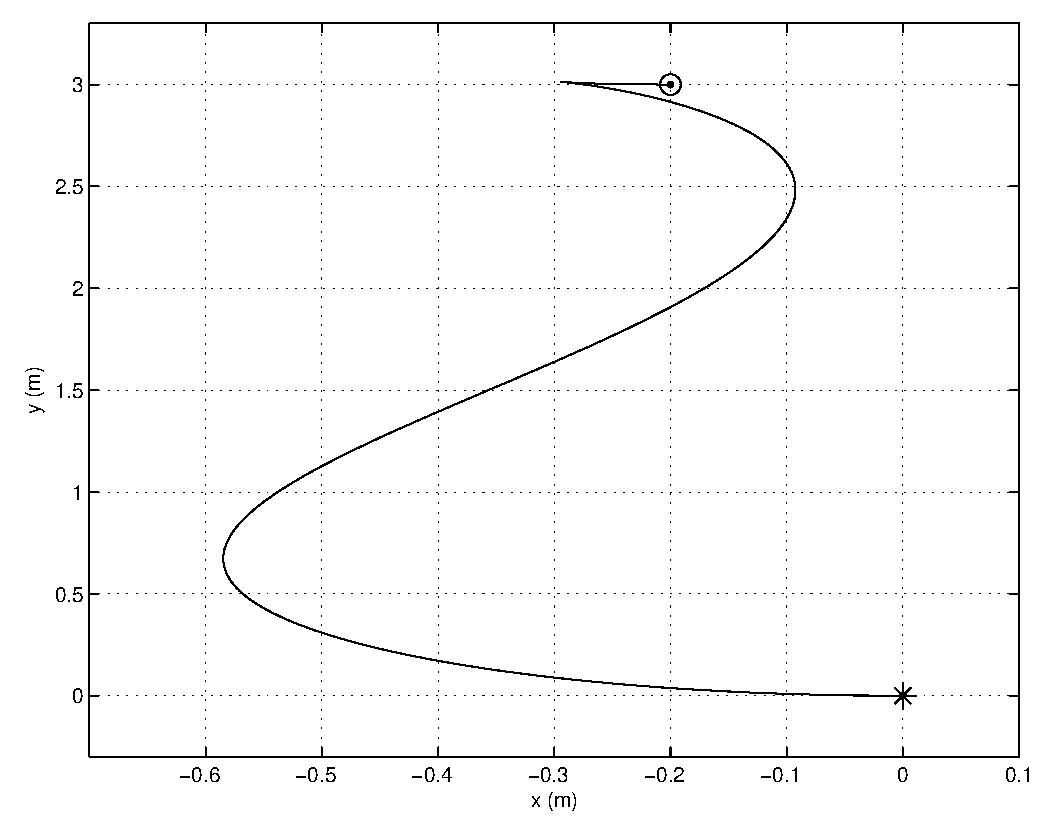
\includegraphics[width=.6\linewidth]{Figuras/sordalen/traj_01.eps}
    \caption{Trajet�ria no plano $XY$. Controle de \cite{sordalen93a}.}
    \label{fig:sordalen_traj_01}
\end{center}\end{figure}
\begin{figure}[H]\begin{center}
    \includegraphics[width=.6\linewidth]{Figuras/sordalen/state_01.eps}
    \caption{Estados $x$, $y$ e $\theta$. Controle de \cite{sordalen93a}.}
    \label{fig:sordalen_state_01}
\end{center}\end{figure}

Da mesma forma apresentada anteriormente, esta lei de controle tamb�m gera uma trajet�ria bastante suave, sem movimentos oscilat�rios desnecess�rios e com uma taxa de converg�ncia bastante elevada. O tempo com que o rob� chega na origem � de apenas 4 segundos. Em~\cite{sordalen93a} � apresentado um roteiro de c�lculo para os par�metros $\gamma$ e $k$ que levam em conta os intervalos de tempo em que $a(t)$ e $\alpha(t)$ devem chegar a um determinado valor final. Assim, pode-se escolher um determinado tempo de acomoda��o e calcular $\gamma$ e $k$ para o caso desejado. Entretanto, este m�todo n�o leva em considera��o as amplitudes das entradas de controle, e conforme os valores dos par�metros, estas amplitudes podem ser tais que ultrapassem os limites aceit�veis, o que efetivamente ocorre, neste caso, para o rob� Twil\footnote{Os limites para o rob� Twil s�o de $0,4712~m/s$ para a velocidade linear e de $3,7699~rad/s$ para a velocidade angular. Maiores detalhes s�o descritos no Ap�ndice~\ref{app:twil}.}~(Figura~\ref{fig:sordalen_control_01}).

\begin{figure}[H]\begin{center}
    \includegraphics[width=.6\linewidth]{Figuras/sordalen/control_01.eps}
    \caption{Entradas de controle $v$ e $w$. Controle de \cite{sordalen93a}.}
    \label{fig:sordalen_control_01}
\end{center}\end{figure}

% CAP�TULO 3
\chapter{Fundamentos de Controle Preditivo Baseado em Modelo}\label{cap:mpc}
%%%%%%%%%%%%%%%%%%%%
\section{Introdu��o}
Desde os anos 70, o MPC tem recebido cada vez mais aten��o, tanto da comunidade acad�mica quanto de empresas interessadas em aplic�-lo em suas plantas industriais. Embora estas duas vertentes tenham seguido, de certa forma, caminhos diferentes, estes caminhos convergem atualmente para objetivos bastante comuns. Inicialmente, quest�es de cunho mais te�rico como garantia de estabilidade e robustez foram, em primeiro momento, deixadas de lado frente ao bom desempenho pr�tico de tais leis. Por outro lado, a partir da d�cada de 90, o grande interesse da ind�stria no MPC levou a comunidade acad�mica a desenvolver trabalhos te�ricos, envolvendo provas de estabilidade, robustez, diferentes esquemas para modelagem dos sistemas e a utiliza��o de observadores de estados, por exemplo.

Da mesma forma, a evolu��o dos computadores e de algoritmos num�ricos de otimiza��o t�m feito com que o MPC possa ser considerado tamb�m para aplica��es em sistemas de din�micas r�pidas ou de dimens�es elevadas. Em sistemas eletromec�nicos, o interesse recai principalmente na possibilidade que o MPC proporciona em se considerar restri��es nos estados e nas entradas de controle, bem como o fato de possuir um crit�rio de otimiza��o que faz com que a lei de controle calculada seja �tima no sentido de que minimiza este crit�rio.

Neste cap�tulo uma descri��o inicial do MPC ser� feita, juntamente com uma breve perspectiva hist�rica, situando o desenvolvimento do controle preditivo ao longo do tempo. Logo ap�s, o MPC � formulado matematicamente em suas duas vers�es, linear e n�o linear, ambas discretas no tempo. A �ltima se��o deste cap�tulo trata de trabalhos j� desenvolvidos onde o MPC � utilizado para controlar rob�s m�veis.


%%%%%%%%%%%%%%%%%%%%%%%%%%%%%%%%%%%%%%%%%%%%%%%%%%%%%%%%%
\section{Perspectiva Hist�rica}\label{sec:mpc_historical}
O controle preditivo baseado em modelo, MPC, � uma forma de controle que pode ser usada em sistemas complexos, multivari�veis e com restri��es nas entradas de controle e nos estados. Uma seq��ncia de controle que minimiza uma fun��o de custo � calculada {\em on-line}, a cada instante de amostragem, atrav�s da resolu��o de um problema de otimiza��o com um horizonte finito de predi��o, usando o estado corrente da planta como condi��o inicial. Assim, obt�m-se uma seq��ncia �tima de controle dentro daquele horizonte sendo que apenas o primeiro elemento desta seq��ncia � aplicada no processo~\cite{mayne00}. A seguir, estas etapas se repetem em uma pol�tica de horizonte deslizante ({\em receding horizon}), o que confere uma caracter�stica de malha fechada � lei de controle gerada.

Em m�todos de controle �timo como o ${\cal H}_2$ e ${\cal H}_\infty$, uma solu��o anal�tica existe e pode ser calculada {\em off-line} atrav�s da resolu��o de equa��es de Ricatti~\cite{kwakernaak72}. Entretanto, estes m�todos s�o v�lidos apenas para sistemas lineares e sem restri��es. Essencialmente, a diferen�a � que no MPC restri��es existentes nos estados e nas entradas de controle s�o consideradas e a otimiza��o � resolvida {\em on-line} para cada instante de amostragem. Torna-se assim necess�rio um horizonte finito para o c�lculo da lei de controle. Assim, em princ�pio, n�o existe uma solu��o anal�tica e a lei de controle � dada implicitamente para cada instante de amostragem.

Uma t�cnica bastante recente, desenvolvida em~\cite{bemporad02,tondel03}, garante uma express�o anal�tica expl�cita para o MPC considerando um sistema linear em tempo discreto, com um crit�rio quadr�tico de minimiza��o e com restri��es em um horizonte finito de predi��o. Esta express�o anal�tica � obtida a partir de programa��o quadr�tica multi-param�trica ({\em multi-parametric Quadratic Program, mp-QP}). Atrav�s da parti��o do espa�o de estados em sub-regi�es poliedrais convexas, uma solu��o linear afim e cont�nua por partes do tipo ${\bf u}={\bf Kx}+{\bf c}$ � encontrada para cada sub-regi�o do espa�o de estados, onde $\bf K$ � uma matriz de realimenta��o de estados e $\bf c$ � um termo independente. Segundo os autores, esta t�cnica aumenta a confiabilidade do controle e a solu��o {\em on-line} do problema de otimiza��o n�o precisa mais ser feita, j� que a lei de controle � calculada {\em off-line}, diminuindo assim o esfor�o computacional e permitindo a sua aplica��o em sistemas com din�micas bastante r�pidas. Entretanto, o n�mero de parti��es (sub-regi�es) depende da dimens�o do sistema, e mesmo para sistemas de ordem 2 a quantidade destas parti��es j� � alto, conforme exemplo dos autores. Assim, para sistemas de ordem elevada s�o necess�rios mecanismos de busca em �rvore bastante complexos.

Algums pontos fortes bastante evidentes do MPC com rela��o a outras t�cnicas de controle podem ser citadas~\cite{camacho99}:
\begin{itemize}
	\item Os conceitos s�o intuitivos;
	\item Restri��es e limites do sistema podem ser levados em considera��o durante o c�lculo da lei de controle de uma forma direta;
	\item Pode ser usado em uma ampla gama de processos, incluindo, por exemplo, sistemas multivari�veis, sistemas de fase n�o-m�nima, com longos atrasos de tempo ou que s�o inst�veis em malha aberta;
	\item Aplic�vel a processos onde se conhece os valores futuros de refer�ncia, como sistemas em batelada ({\it batch processes}) ou em rastreamento de trajet�ria;
	\item V�rios tipos de modelos podem ser utilizados: espa�o de estados, fun��o de transfer�ncia, resposta ao impulso, etc.
\end{itemize}

Entretanto, existem tamb�m alguns pontos fracos, a saber:
\begin{itemize}
	\item Necessidade de um modelo preciso do sistema para o c�lculo de valores futuros dos estados. A predi��o dos estados � feita com base neste modelo e � utilizada no crit�rio de minimiza��o;
	\item Alto custo computacional (em cada instante um problema de otimiza��o � resolvido {\em on-line}). Para o caso n�o linear, o problema de otimiza��o � n�o convexo, possui um maior n�mero de vari�veis de decis�o e um m�nimo global geralmente � imposs�vel de se encontrar. Entretanto, se o sistema � linear, a fun��o de custo � quadr�tica e as restri��es s�o lineares, o problema de otimiza��o pode ser transformado em um problema de programa��o quadr�tica ({\em Quadratic Programming, QP}), onde o problema � convexo e uma solu��o �tima sempre existe, pelo menos localmente.
\end{itemize}

Embora as principais aplica��es do MPC tenham se desenvolvido mais recentemente e primeiramente na ind�stria, a id�ia de se controlar um sistema atrav�s de uma seq��ncia de problemas de otimiza��o {\em on-line} n�o � nova. Em 1967, \cite{lee67} anteciparam o que viria a ser, atualmente, a ess�ncia do MPC:
\begin{margins}{1cm}{0cm}
{\small Pode-se obter um controlador por realimenta��o atrav�s do conhecimento de v�rios controladores em malha aberta. Primeiramente mede-se o estado atual do processo e calcula-se muito rapidamente a lei de controle em malha aberta. A primeira por��o deste controle � ent�o aplicada no processo durante um curto per�odo de tempo, depois do qual uma nova lei de controle � calculada baseada nas novas informa��es do processo. O procedimento ent�o repete-se.}\footnote{Traduzido do original em ingl�s pelo autor.}
\end{margins}

Esta id�ia era, a princ�pio, impratic�vel, dada � alta quantidade de c�lculos necess�rios. Contudo, com o advento da computa��o digital, algumas solu��es come�aram a ser implementadas, principalmente nas ind�strias de processo e petroqu�mica, onde considera��es econ�micas (aumento da produtividade e da qualidade dos produtos) tornava necess�rio aproximar os pontos de opera��o das plantas de seus limites, sem que estes fossem, logicamente, ultrapassados. As primeiras aplica��es industriais dispon�veis comercialmente surgiram nas d�cadas de 70  e 80 com, por exemplo, o {\em Model Algorithmic Control, MAC}~\cite{richalet76}, o {\em Dynamic Matrix Control, DMC}~\cite{cutler80}, o {\em Extended Prediction Self Adaptive Control, EPSAC}~\cite{dekeyser85}, o {\em Quadratic Dynamic Matrix Control, QDMC}~\cite{garcia86} e o {\em Generalized Predictive Control, GPC}~\cite{clarke87}, todos para plantas lineares. Cabe ressaltar que, com excess�o do GPC, todas as outras s�o aplic�veis somente em plantas est�veis em malha aberta.

Em aplica��es industriais para processos n�o lineares, existem atualmente, por exemplo, o NOVA~\cite{dynamic96} e o Process Perfector~\cite{martin97}, mas por serem tecnologias propriet�rias, detalhes dos algoritmos n�o existem na literatura.

V�rias refer�ncias sobre o MPC quanto � teoria e aplica��es industriais podem ser vistos em \cite{garcia89,qin97,morari97,henson98,allgower99,camacho99,qin00,rawlings00,rossiter03}.

As primeiras vers�es do MPC na ind�stria n�o levavam em conta a estabilidade do sistema em malha fechada, mas obviamente sabia-se que esta era uma quest�o importante. Propriedades associadas a um controle com horizonte infinito eram garantidas restringindo a aplica��o para plantas est�veis em malha aberta e escolhendo um horizonte de predi��o suficientemente grande. Assim, estimulada pelo grande sucesso do MPC na ind�stria, a comunidade acad�mica preocupou-se em abordar quest�es te�ricas n�o estudadas at� ent�o. Inicialmente, t�cnicas baseadas na teoria de Lyapunov foram negligenciadas, mas ganharam for�a com o trabalho de \cite{chen82}, que mostrou que a fun��o de custo de um problema de controle �timo com horizonte finito pode ser usada como uma fun��o de Lyapunov para sistemas em tempo cont�nuo e sem restri��es. Em \cite{keerthi88}, estes resultados foram estendidos para sistemas n�o lineares em tempo discreto, variantes no tempo e com restri��es. Depois destes trabalhos, v�rios outros abordando estabilidade do MPC foram desenvolvidos, como por exemplo \cite{mayne90,bitmead90,michalska93,chen98,mayne00}


%%%%%%%%%%%%%%%%%%%%%%%%%%%%%%%%%%%%%%%%%%%%%%%%%%%%%%
\section{Elementos Essenciais}\label{sec:mpc_elements}
Uma analogia do MPC pode ser feita ao ato de se dirigir um autom�vel~\cite{camacho99}. O motorista sabe a trajet�ria de refer�ncia desejada para um horizonte finito: seu campo de vis�o da estrada. Levando em conta as caracter�sticas do carro (um {\em modelo mental} do carro e limita��es de velocidade, acelera��o e manobrabilidade) bem como poss�veis obst�culos na estrada (como buracos, cruzamentos e outros carros), ele decidir� que a��o tomar (aumentar ou diminuir a velocidade, girar a dire��o para um lado ou para outro) a fim de que a desejada trajet�ria seja percorrida. Esta a��o de controle � ent�o aplicada por um curto espa�o de tempo e o procedimento se repete para a pr�xima a��o de controle, agora com o seu campo de vis�o atualizado. Observa-se que, utilizando o modelo do carro, predi��es de comportamento s�o utilizadas, baseadas no que o motorista est� enxergando � sua frente. 

Todas as vers�es de MPC possuem assim elementos comuns que podem ser escolhidos de diferentes formas, conforme as necessidades e a aplica��o. Estes elementos s�o~\cite{camacho99}:
\begin{itemize}
\item {\em Modelo de predi��o.} O modelo do processo � a pe�a-chave do MPC. Seu uso � determinado pela necessidade de se {\em predizer} os estados (ou sa�das) do sistema em instantes de tempo no futuro. As diferentes estrat�gias de controle preditivo podem utilizar diferentes tipos de modelos para representar a rela��o entre as entradas de controle e os estados (ou sa�das) do sistema, como modelos por resposta ao impulso (usado no MAC), resposta ao degrau (usado no DMC e QDMC), fun��o de transfer�ncia (usado no GPC) e espa�o de estados (que ser� utilizado neste trabalho). A vantagem deste �ltimo � que a formula��o do MPC pode ser estendida para processos multivari�veis e n�o lineares de uma forma bastante direta. 

Em situa��es realistas, onde geralmente existem diferen�as entre o processo e seu modelo, � preciso identificar tamb�m um modelo para as incertezas, sendo assim as duas partes necess�rias para a predi��o.

\item {\em Fun��o de custo.} � o crit�rio de desempenho com rela��o ao qual ser� feita a otimiza��o da lei de controle. As v�rias formula��es do MPC utilizam diferentes tipos de fun��o de custo. A id�ia predominante � que esta fun��o de custo � formada por um somat�rio de termos dos estados (ou sa�das) e das entradas de controle ao longo do horizonte. Assim, a minimiza��o desta fun��o implica na minimiza��o do erro nas vari�veis de estado e de controle. Esta fun��o pode ainda incluir outros termos como penaliza��es na varia��o do esfor�o de controle e custo terminal dos estados.

\item {\em Obten��o da lei de controle.} Para se obter uma seq��ncia de valores �timos das vari�veis de decis�o dentro do horizonte de predi��o, realiza-se a minimiza��o da fun��o de custo, ou seja, o c�lculo do valor m�nimo desta fun��o atrav�s da manipula��o das vari�veis de decis�o. Para fazer isso, usa-se o modelo do sistema para calcular valores futuros dos estados ou das sa�das. Geralmente as vari�veis de decis�o s�o as entradas de controle. No caso n�o linear, tanto os estados quanto o controle s�o vari�veis de decis�o. Se existirem restri��es, a minimiza��o da fun��o de custo precisa respeit�-las. A lei de controle � ent�o dada implicitamente pelo primeiro termo da seq��ncia calculada.

\item {\em Horizonte deslizante.} At� a obten��o da lei de controle, o MPC funciona essencialmente como um m�todo de controle em malha aberta: calcula uma lei de controle para o estado atual da planta atrav�s da minimiza��o da fun��o de custo. Entretanto, em sua totalidade, a estrat�gia funciona em malha fechada, pois, atrav�s da aplica��o do controle calculado em cada instante de amostragem, os estados do sistema s�o atualizados e o processo de otimiza��o e do c�lculo da lei de controle se repete, agora com o instante de amostragem deslocado em uma unidade para o futuro, o que d� a caracter�stica de horizonte m�vel ou deslizante.
\end{itemize}

Todas estas id�ias s�o ent�o expostas formalmente nas pr�ximas se��es.


%%%%%%%%%%%%%%%%%%%%%%%%%%%%%%%%%%%%%%
\section{Formula��o do MPC N�o Linear}

Se o modelo do sistema � n�o linear ou se existirem restri��es n�o lineares a serem respeitadas, o problema de minimiza��o a ser resolvido em cada instante de amostragem � n�o linear, configurando-se assim um MPC n�o linear ({\em Nonlinear Model-based Predictive Control, NMPC}). No NMPC, as vari�veis de decis�o s�o as vari�veis de estado e de controle, e o comportamento din�mico do sistema � respeitado atrav�s da imposi��o de uma restri��o n�o linear na forma do modelo deste sistema.

Assim, ser� considerado aqui um sistema com o seguinte modelo:
\begin{equation}\label{eqn:mpc_nl_model}
	\dot{\bf x}(t) = f({\bf x}(t),{\bf u}(t)),
\end{equation}
onde $\bf x$ � o vetor de estados de ordem $n$, ${\bf x}\in\real^n$, $\bf u$ � o vetor de entradas de controle de ordem $m$, ${\bf u}\in\real^m$ e $t$ � o tempo. Em tempo discreto, o modelo acima pode ser representado pela seguinte equa��o de diferen�as:
\begin{equation}\label{eqn:mpc_nl_model_discrete}
	{\bf x}(k+1) = f({\bf x}(k),{\bf u}(k)),
\end{equation}
onde $k$ � o instante de amostragem, $k = \{k|k\in{\mathbb N},k\geq 0\}$.

A fun��o de custo a ser minimizada tem a forma
\begin{equation}\label{eqn:cost}
	\Phi(k) = \sum_{j=N_1}^{N_2}{\bf x}^T(k+j|k){\bf Q}{\bf x}(k+j|k) + \sum_{j=1}^{N_u}{\bf u}^T(k+j|k){\bf R}{\bf u}(k+j|k),
\end{equation}
onde $N=N_2-N_1+1$ � o {\em horizonte de predi��o} e $N_u$ � o {\em horizonte de controle}. ${\bf Q}$ e ${\bf R}$ s�o matrizes de pondera��o utilizadas para penalizar o erro de estado e o esfor�o de controle, respectivamente, com ${\bf Q}\geq 0$ e ${\bf R}>0$.

Como dito anteriormente, na pr�tica todo o sistema est� sujeito a restri��es, estas podendo surgir quando da exist�ncia de basicamente tr�s tipos de limita��es:
\begin{itemize}
\item {\it Limites f�sicos}. Quando existem barreiras f�sicas que n�o podem ser ultrapassadas, como por exemplo, faixas de atua��o de atuadores e sensores, vaz�o m�xima de tubula��es, etc.;
\item {\it Limites de seguran�a}. Limites que se ultrapassados podem levar a situa��es de perigo, como explos�es ou desastres ambientais;
\item {\it Limites operacionais}. Relativos ao desempenho do sistema e � qualidade do produto final. S�o restri��es que, eventualmente, podem ser violadas a fim de se preservar as restri��es relativas aos limites f�sicos ou de seguran�a.
\end{itemize}

Assim, definem-se, de uma forma geral, as seguintes express�es de restri��o:

\begin{align*}
	{\bf x}(k+j|k) &\in \mathbb{X}, \quad j\in[N_1,N_2] \\
	{\bf u}(k+j|k) &\in \mathbb{U}, \quad j\in[0,N_u]
\end{align*}
onde $\mathbb{X}$, fechado e convexo, � o conjunto dos poss�veis valores para os estados do sistema e $\mathbb{U}$, compacto e convexo, � o conjunto das poss�veis entradas de controle. Se forem lineares com rela��o a $\bf x$ e $\bf u$, as restri��es podem ser escritas como:
\begin{align}
	{\bf Cx}(k+j|k) &\leq {\bf c}, \quad j\in[N_1,N_2] \label{eqn:restx} \\
	{\bf Du}(k+j|k) &\leq {\bf d}, \quad j\in[0,N_u] \label{eqn:restu}
\end{align}
com ${\bf C}\in\real^{l_{{\bf x}}\times n}$, ${\bf c}\in\real^{l_{{\bf x}}}$, ${\bf D}\in\real^{l_{{\bf u}}\times m}$ e ${\bf d}\in\real^{l_{{\bf u}}}$.

Assim, o problema de otimiza��o a ser resolvido em cada instante de amostragem $k$ pode ser posto como encontrar uma seq��ncia de controle ${\bf u}^\star$ e uma seq��ncia de estados ${\bf x}^\star$ tal que minimizem a fun��o de custo $\Phi(k)$ e respeitem as restri��es impostas, ou seja:
\begin{equation}\label{eqn:optim}
	{\bf u}^\star,~{\bf x}^\star = \arg\min_{{\bf u},{\bf x}}\left\{\Phi(k)\right\}
\end{equation}
sujeito a:
\begin{alignat*}{2}
	{\bf x}(k|k)    &= {\bf x}_0, \\
	{\bf x}(k+j|k)  &= f({\bf x}(k+j-1|k),{\bf u}(k+j-1|k)), &\quad &j \in[N_1,N_2] \\
	{\bf Cx}(k+j|k) &\leq {\bf c}, &\quad &j \in[N_1,N_2] \\
	{\bf Du}(k+j|k) &\leq {\bf d}, &\quad &j \in[0,N_u]
\end{alignat*}
onde ${\bf x}_0$ � a condi��o inicial, ou seja, o valor medido de $\bf x$ no instante $k$. O problema~\req{eqn:optim} � ent�o resolvido para cada instante de amostragem $k$, resultando em uma seq��ncia �tima de controle
\begin{equation}\label{eqn:control_seq}
	{\bf u}^\star = \{{\bf u}^\star(k|k),{\bf u}^\star(k+1|k),{\bf u}^\star(k+2|k),\ldots,{\bf u}^\star(k+N_u|k)\},
\end{equation}
uma seq��ncia �tima de estados
\begin{equation}\label{eqn:state_seq}
	{\bf x}^\star = \{{\bf x}^\star(k+N_1|k),{\bf x}^\star(k+N_1+1|k),{\bf x}^\star(k+N_1+2|k),\ldots,{\bf x}^\star(k+N_2|k)\}
\end{equation}
e um custo �timo $\Phi^\star(k)$. Assim, a lei de controle do MPC � dada implicitamente pelo primeiro termo da seq��ncia ${\bf u}^\star$:
\begin{equation}\label{eqn:control_law}
	h(\delta) = {\bf u}^\star(k|k),
\end{equation}
onde $h(\delta)$ � cont�nua dentro de cada per�odo de amostragem $T$, $\delta\in[kT,(k+1)T)$. O resto da seq��ncia ${\bf u}^\star$ � descartada. Logo, o sistema~\req{eqn:mpc_nl_model}, em malha fechada, pode ser escrito como:
\begin{equation}\label{mpc_closed_loop}
	\dot{\bf x}(\delta) = f({\bf x}(\delta),h(\delta))
\end{equation}	

No pr�ximo instante de amostragem ($k+1$), todo o procedimento se repete, agora com os estados atualizados pela express�o~\req{mpc_closed_loop} e uma janela de tempo deslocada em um instante de amostragem para frente (horizonte deslizante). O comportamento do MPC ao longo do horizonte pode ser visto genericamente na Figura~\ref{fig:mpc}.

O problema com otimiza��es n�o lineares � a sua n�o convexidade, existindo assim v�rios m�nimos locais, o que faz com que, geralmente, seja imposs�vel achar um m�nimo global, gerando assim solu��es sub-�timas~\cite{henson98}. Ainda, o custo computacional � exponencialmente relacionado com o n�mero de vari�veis de decis�o~\cite{henrion04}. Assim, dependendo da rapidez da din�mica ou de sua dimens�o, a aplica��o do MPC em um sistema n�o linear pode tornar-se impratic�vel.

Em particular, neste trabalho, ser� utilizada a fun��o {\tt fmincon} do pacote de otimiza��o do Matlab para a resolu��o de problemas de otimiza��o n�o linear. Para a solu��o de um problema de programa��o n�o linear\footnote{Um problema de programa��o n�o linear � um problema de otimiza��o onde a fun��o de custo a ser minimizada e as restri��es s�o n�o lineares.}~\cite{luenberger89}, a fun��o {\tt fmincon} utiliza o m�todo {\em Quasi-Newton} com um procedimento de busca polinomial de ordens quadr�tica e c�bica. Este m�todo utiliza a formula��o BFGS~\cite{broyden70,fletcher70,goldfarb70,shanno70} para calcular uma aproxima��o da matriz Hessiana em cada itera��o do processo de otimiza��o. Assim, resolve-se um sub-problema atrav�s do m�todo {\em Active Set}, chamado de Programa��o Quadr�tica Sequencial ({\em Sequential Quadratic Programming, SQP})~\cite{fletcher87,gil81,hock83} baseada em uma aproxima��o quadr�tica da fun��o Lagrangiana. A solu��o de cada SQP � ent�o utilizada para calcular uma dire��o de busca do ponto �timo.

\begin{figure}\begin{center}
    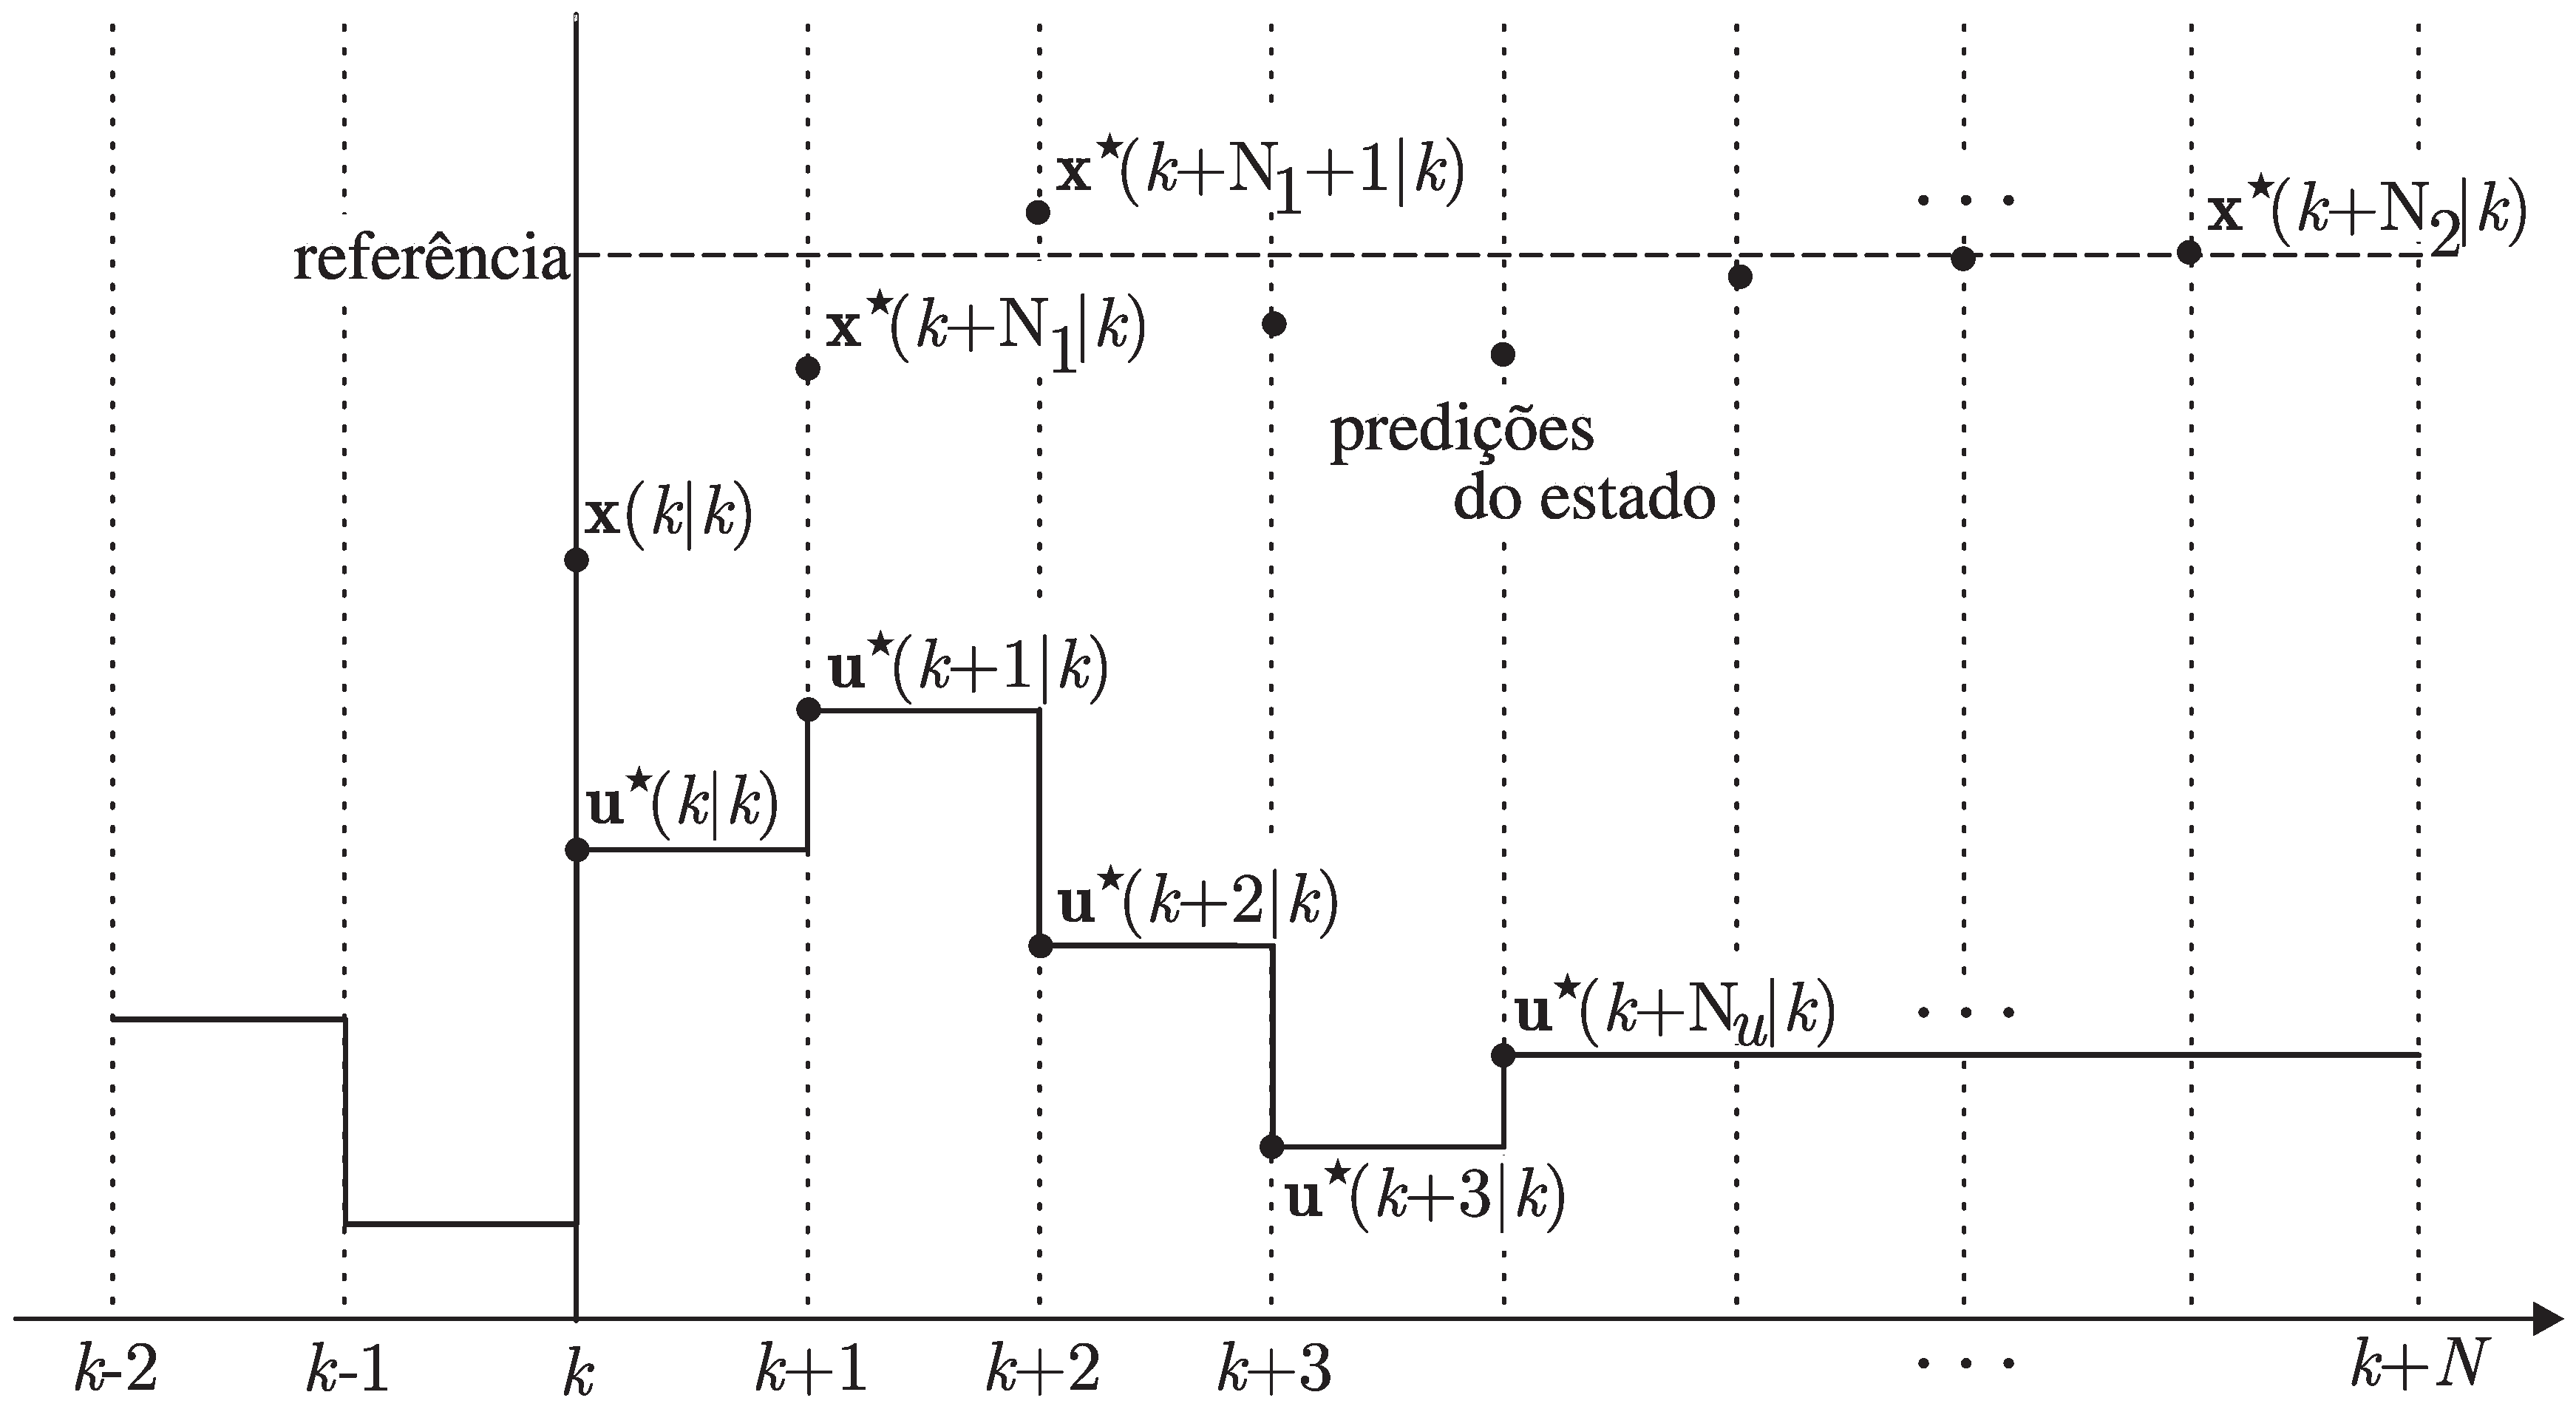
\includegraphics[width=\linewidth]{Figuras/mpc.eps}
    \caption{O controle preditivo.}
    \label{fig:mpc}
\end{center}\end{figure}


%%%%%%%%%%%%%%%%%%%%%%%%%%%%%%%%%%%%%%%%%%%%%%%%%%
\section{Formula��o do MPC Linear}\label{sec:lmpc}

Se o modelo do sistema � linear e existirem apenas restri��es lineares a serem respeitadas, pode-se formular o MPC de forma linear ({\em Linear Model-based Predictive Control, LMPC}). Assim, considerando as entradas de controle como as vari�veis de decis�o e tendo-se um crit�rio quadr�tico de minimiza��o, pode-se transformar o problema de minimiza��o em um problema de programa��o quadr�tica, QP, para o qual algoritmos num�ricos robustos e eficientes existem. Problemas de otimiza��o deste tipo t�m a vantagem, quando comparados com problemas n�o lineares, de serem convexos, o que faz com que sempre exista um m�nimo global.

Assim, reescreve-se a express�o~\req{eqn:mpc_nl_model_discrete}, referente ao modelo din�mico do sistema, na forma linear, discreta e invariante no tempo:
\begin{equation}\label{eqn:mpc_linear_model}
	{\bf x}(k+1) = {\bf Ax}(k) + {\bf Bu}(k),
\end{equation}
onde $\bf A$ � a matriz de transi��o de estados e $\bf B$ � a matriz que relaciona os estados com as entradas de controle. Pode-se prever o estado do sistema para um instante de amostragem $j$ no futuro atrav�s da aplica��o recursiva da express�o~\req{eqn:mpc_linear_model}:
\begin{align*}
	{\bf x}(k+1|k) &= {\bf Ax}(k|k) + {\bf Bu}(k|k) \\
	{\bf x}(k+2|k) &= {\bf A}^2{\bf x}(k|k) + {\bf ABu}(k|k) + {\bf Bu}(k+1|k) \\
	{\bf x}(k+3|k) &= {\bf A}^3{\bf x}(k|k) + {\bf A}^2{\bf Bu}(k|k) + {\bf A}{\bf Bu}(k+1|k) + {\bf Bu}(k+2|k) \\
	&\vdots \\
	{\bf x}(k+j|k) &= {\bf A}^j{\bf x}(k|k) + \sum_{i=0}^{j-1}{\bf A}^{j-1-i}{\bf Bu}(k+i|k) 
\end{align*}

Sem perda de generalidade e a fim de simplificar a formula��o matem�tica, escolhe-se, na express�o~\req{eqn:cost}, $N_1=1$, $N_2=N$ e $N_u=N-1$ e tem-se a seguinte fun��o de custo:
\begin{equation*}
	\Phi(k) = \sum_{j=1}^{N}{\bf x}^T(k+j|k){\bf Q}{\bf x}(k+j|k) + {\bf u}^T(k+j-1|k){\bf R}{\bf u}(k+j-1|k)
\end{equation*}

Definido os seguintes vetores:
\begin{equation*}
	\bar{\bf x}(k+1|k) = \begin{bmatrix}
		{\bf x}(k+1|k) \\ {\bf x}(k+2|k) \\ \vdots \\ {\bf x}(k+N|k)
	\end{bmatrix} \quad {\text e} \quad
	\bar{\bf u}(k|k) = \begin{bmatrix}
		{\bf u}(k|k) \\ {\bf u}(k+1|k) \\ \vdots \\ {\bf u}(k+N-1|k)
	\end{bmatrix},
\end{equation*}
pode-se reescrever a fun��o de custo como:
\begin{equation*}
	\Phi(k) = \bar{\bf x}^T(k+1|k)\bar{\bf Q}\bar{\bf x}(k+1|k) + \bar{\bf u}^T(k|k)\bar{\bf R}\bar{\bf u}(k|k),
\end{equation*}
onde
\begin{equation*}
	\bar{\bf Q} = \begin{bmatrix}
		{\bf Q} & {\bf 0} & \cdots & {\bf 0} \\
		{\bf 0} & {\bf Q} & \cdots & {\bf 0} \\
		\vdots  & \vdots  & \ddots & \vdots  \\
		{\bf 0} & {\bf 0} & \cdots & {\bf Q} \\
	\end{bmatrix} \quad {\text e} \quad
	\bar{\bf R} = \begin{bmatrix}
		{\bf R} & {\bf 0} & \cdots & {\bf 0} \\
		{\bf 0} & {\bf R} & \cdots & {\bf 0} \\
		\vdots  & \vdots  & \ddots & \vdots  \\
		{\bf 0} & {\bf 0} & \cdots & {\bf R} \\
	\end{bmatrix}
\end{equation*} 

Fazendo
\begin{equation*}
	\bar{\bf x}(k+1|k) = \bar{\bf A}{\bf x}(k|k) + \bar{\bf B}\bar{\bf u}(k|k),
\end{equation*}
onde
\begin{equation*}
	\bar{\bf A} = \begin{bmatrix}
		{\bf A} \\ {\bf A}^2 \\ \vdots \\ {\bf A}^{N-1} \\ {\bf A}^N
	\end{bmatrix} \quad {\text e} \quad
	\bar{\bf B} = \begin{bmatrix}
		{\bf B} & {\bf 0} & {\bf 0} & \cdots & {\bf 0} \\
		{\bf AB} & {\bf B} & {\bf 0} & \cdots & {\bf 0} \\
		\vdots & \vdots & \vdots & \ddots & \vdots \\
		{\bf A}^{N-2}{\bf B} & {\bf A}^{N-3}{\bf B} & {\bf A}^{N-4}{\bf B}& \cdots & {\bf 0} \\
		{\bf A}^{N-1}{\bf B} & {\bf A}^{N-2}{\bf B} & {\bf A}^{N-3}{\bf B}& \cdots & {\bf B}
	\end{bmatrix},
\end{equation*}
tem-se que:
\begin{equation*}
	\Phi(k) = \left({\bf x}^T(k|k)\bar{\bf A}^T + \bar{\bf u}^T(k|k)\bar{\bf B}^T\right)\bar{\bf Q}\left(\bar{\bf A}{\bf x}(k|k)+\bar{\bf B}\bar{\bf u}(k|k)\right) + \bar{\bf u}^T(k|k)\bar{\bf R}\bar{\bf u}(k|k)
\end{equation*}
e
\begin{multline*}	
	\Phi(k) = {\bf x}^T(k|k)\bar{\bf A}^T\bar{\bf Q}\bar{\bf A}{\bf x}(k|k) + {\bf x}^T(k|k)\bar{\bf A}^T\bar{\bf Q}\bar{\bf B}\bar{\bf u}(k|k) + \\ + \bar{\bf u}^T(k|k)\bar{\bf B}^T\bar{\bf Q}\bar{\bf A}{\bf x}(k|k) + \bar{\bf u}^T(k|k)\bar{\bf B}^T\bar{\bf Q}\bar{\bf B}\bar{\bf u}(k|k) + \bar{\bf u}^T(k|k)\bar{\bf R}\bar{\bf u}(k|k)
\end{multline*}

Os termos quadr�ticos em $\bar{\bf u}(k|k)$ s�o:
\begin{align*}
	\bar{\bf u}^T(k|k)\bar{\bf B}^T\bar{\bf Q}\bar{\bf B}\bar{\bf u}(k|k) + \bar{\bf u}^T(k|k)\bar{\bf R}\bar{\bf u}(k|k) &= \bar{\bf u}^T(k|k)\left(\bar{\bf B}^T\bar{\bf Q}\bar{\bf B}+\bar{\bf R}\right)\bar{\bf u}(k|k) \\
	   &= \frac{1}{2}\bar{\bf u}^T(k|k)\bar{\bf H}\bar{\bf u}(k|k),
\end{align*}
os termos lineares em $\bar{\bf u}(k|k)$ s�o:
\begin{align*}
	{\bf x}^T(k|k)\bar{\bf A}^T\bar{\bf Q}\bar{\bf B}\bar{\bf u}(k|k) + \bar{\bf u}^T(k|k)\bar{\bf B}^T\bar{\bf Q}\bar{\bf A}{\bf x}(k|k) &= 2{\bf x}^T(k|k)\bar{\bf A}^T\bar{\bf Q}\bar{\bf B}\bar{\bf u}(k|k) \\
					 &= {\bf f}^T\bar{\bf u}(k|k)
\end{align*}
e o termo independente de $\bar{\bf u}(k|k)$ � ${\bf x}^T(k|k)\bar{\bf A}^T\bar{\bf Q}\bar{\bf A}{\bf x}(k|k)$. Assim, a fun��o de custo pode ser escrita em uma forma quadr�tica padr�o:
\begin{equation}\label{eqn:quadratic_form}
	\Phi(k) = \frac{1}{2}\bar{\bf u}^T(k|k)\bar{\bf H}\bar{\bf u}(k|k) + {\bf f}^T\bar{\bf u}(k|k) + {\bf g},
\end{equation}
com
\begin{align*}
		{\bf H} &= 2\left(\bar{\bf B}^T\bar{\bf Q}\bar{\bf B}+\bar{\bf R}\right) \\
		{\bf f} &= 2\bar{\bf B}^T\bar{\bf Q}\bar{\bf A}{\bf x}(k|k) \\
		{\bf g} &= {\bf x}^T(k|k)\bar{\bf A}^T\bar{\bf Q}\bar{\bf A}{\bf x}(k|k)
\end{align*}
e $\bf g$ � independente de $\bar{\bf u}(k|k)$ e n�o importa para o problema de minimiza��o. Assim, define-se
\begin{equation}\label{eqn:quadratic_form2}
	\Phi'(k) = \frac{1}{2}\bar{\bf u}^T(k|k)\bar{\bf H}\bar{\bf u}(k|k) + {\bf f}^T\bar{\bf u}(k|k)
\end{equation}

A express�o~\req{eqn:quadratic_form2} � a forma padr�o para se aplicar um algoritmo de QP~~\cite{luenberger89}. Assim, o seguinte problema de otimiza��o � resolvido em cada instante de amostragem $k$:
\begin{equation}\label{eqn:linopt2}
	{\bf u}^\star = \arg\min_{\bf u}\left\{\Phi'(k)\right\}
\end{equation}
sujeito a:
\begin{equation*}
	{\bf Du}(k+j|k) \leq {\bf d}, \quad j\in[0,N-1]
\end{equation*}

Nota-se que agora, ao contr�rio do NMPC, a �nica vari�vel de decis�o existente, utilizada para minimizar $\Phi'(k)$, � a entrada de controle $\bf u$. Assim, todas as restri��es a serem respeitadas precisam ser escritas com rela��o a esta vari�vel. Ainda, a din�mica linear do sistema~\req{eqn:mpc_linear_model} e a condi��o inicial ${\bf x}(k|k)={\bf x}_0$ est�o embutidas na forma quadr�tica da fun��o de custo, express�o~\req{eqn:quadratic_form}. Este fato simplifica de forma significativa o processo de minimiza��o, diminuindo consideravelmente o esfor�o computacional.

A minimiza��o de $\Phi'(k)$ leva a uma seq��ncia �tima de controle
\begin{equation*}
	{\bf u}^\star = \{{\bf u}^\star(k|k),{\bf u}^\star(k+1|k),{\bf u}^\star(k+2|k),\ldots,{\bf u}^\star(k+N-1|k)\}
\end{equation*}
e um custo �timo $\Phi^\star(k)=\Phi'^\star(k)+{\bf g}$. A lei de controle do MPC � dada implicitamente pelo primeiro termo da seq��ncia ${\bf u}^\star$:
\begin{equation*}
	h(\delta) = {\bf u}^\star(k|k),
\end{equation*}
onde $h(\delta)$ � cont�nua dentro de cada per�odo de amostragem $T$, $\delta\in[kT,(k+1)T)$. O resto da seq��ncia ${\bf u}^\star$ � descartada. O sistema em malha fechada pode ent�o ser escrito em tempo cont�nuo como:
\begin{equation*}
	\dot{\bf x}(\delta) = {\bf Ax} + {\bf B}h(\delta)
\end{equation*}

Conforme mencionado, o problema de otimiza��o~\req{eqn:linopt2} a ser resolvido em cada instante de amostragem neste caso � um problema de Programa��o Quadr�tica, ou seja, o crit�rio a ser minimizado � quadr�tico e as restri��es s�o lineares. A vantagem deste tipo de problema � que o mesmo � convexo e para isto algoritmos eficientes e confi�veis existem. Em geral, estes algoritmos s�o baseados na solu��o das equa��es de Kuhn-Tucker que, neste caso, d�o condi��es necess�rias e suficientes de otimalidade~\cite{luenberger89}.

Em particular, neste trabalho ser� utilizada a fun��o {\tt quadprog} do pacote de otimiza��o do Matlab para a solu��o de problemas de QP. Esta fun��o soluciona o problema de otimiza��o de otimiza��o atrav�s do m�todo {\em Active Set}, ou m�todo de proje��o~\cite{gil81}. Uma solu��o inicial fact�vel � calculada atrav�s da solu��o de um problema simplificado de Programa��o Linear ({\em Linear Programming, LP}). Em um segundo momento, � gerada uma seq��ncia iterativa de pontos fact�veis que convergem para a solu��o Com o m�todo {\em Active Set}, a fun��o de custo � minimizada em cada itera��o com rela��o a um sub-conjunto de restri��es localmente ativas, at� que o algoritmo encontre a solu��� final.


%%%%%%%%%%%%%%%%%%%%%%%%%%%%%%%%%%%%%
\section{MPC Aplicado a Rob�s M�veis}

Como dito anteriormente, trabalhos envolvendo MPC de rob�s m�veis n�o holon�micos s�o relativamente raros e esparsos. Alguns s�o descritos brevemente a seguir.

Em \cite{ollero91} o GPC � aplicado ao problema de seguimento de caminho do rob� CMU NavLab. Um modelo CARIMA ({\em Controlled Autoregressive and Moving Average}) em coordenadas locais linearizadas do rob� � utilizado para o c�lculo da dist�ncia do rob� a uma trajet�ria de refer�ncia. O controle � realizado apenas atrav�s da velocidade angular, considerando que a velocidade linear permanece constante. Como o modelo utilizado � linear, trajet�rias de aproxima��o do ve�culo � refer�ncia tornam-se necess�rias quando o erro de orienta��o � muito grande. A fun��o de custo envolve o erro de posi��o e orienta��o em coordenadas locais e incrementos do controle e uma restri��o na velocidade linear de 30~{\em km/h} � imposta.

Em \cite{ortega96}, algoritmos gen�ticos s�o utilizados para a otimiza��o n�o linear, a fim de diminuir o esfor�o computacional e tornando poss�vel assim a aplica��o em tempo-real. O problema de rastreamento de trajet�ria � resolvido para um rob� com modelo n�o linear e acionamento diferencial. A novidade neste trabalho � a inclus�o, na fun��o de custo, de um termo que penaliza a proximidade entre o rob� e obst�culos fixos no ambiente. Assim, uma trajet�ria de refer�ncia � previamente calculada, levando em considera��o apenas obst�culos conhecidos. O problema de rastreamento � ent�o resolvido, agora ent�o com obst�culos inesperados presentes no ambiente. O algoritmo foi aplicado ao rob� LABMATE.

Em \cite{yang98} um controle preditivo inteligente � desenvolvido. Um modelo cinem�tico em redes neurais � utilizado para a predi��o dos estados, onde as entradas de controle s�o as velocidades linear e angular. O tipo de rob� utilizado � parecido com um carro, com duas rodas frontais orient�veis e duas rodas n�o-orient�veis traseiras motorizadas. Para corrigir erros existentes entre o modelo de predi��o e o rob� real, uma rede neural � utilizada para ajustar este modelo de forma {\em on-line}. A fun��o de custo envolve termos de erro entre a postura atual e a de refer�ncia e de esfor�o de controle. O problema de seguimento de caminho � resolvido e aplicado ao rob� THMR-III.

\cite{rico99} destaca algumas vantagens da utiliza��o do MPC para o seguimento de caminho de rob�s m�veis, como por exemplo: a trajet�ria � previamente conhecida; o caminho percorrido � suave; h� um aumento na autonomia do rob�, j� que o esfor�o de controle � minimizado. Este trabalho utiliza o GPC sem restri��es para o seguimento de caminho de um modelo linearizado em coordenadas locais do rob�, onde a velocidade linear � constante, a entrada de controle � a velocidade angular e as sa�das s�o a orienta��o global e a posi��o $y$ em coordenadas locais. A exist�ncia de atrasos de transporte no modelo � considerada. Atrav�s de um preditor de Smith, obt�m-se um aumento da robustez do sistema em malha fechada. Um novo algoritmo de controle preditivo ({\em Smith-Predictor Generalized Predictive Control, SPGPC}) � ent�o proposto e aplicado ao rob� LABMATE.

\cite{essen01} desenvolve um algoritmo n�o linear de MPC em espa�o de estados aplicado a um rob� m�vel com acionamento diferencial para a estabiliza��o em uma postura fixa e rastreamento de trajet�ria. Seu m�todo � ent�o comparado com leis de controle variantes no tempo e descont�nuas, mostrando a efici�ncia do MPC. Algumas modifica��es na fun��o de custo s�o propostas, a fim de aumentar a taxa de converg�ncia sem restri��es adicionais, entretanto detalhes do algoritmo n�o s�o fornecidos. Segundo afirmam os autores, os resultados de simula��o mostram que n�o � poss�vel a aplica��o do MPC n�o linear em rob�s m�veis, dado o alto custo computacional necess�rio. O tempo para a solu��o do problema de otimiza��o � cerca de 500 vezes maior que o permitido a uma aplica��o em tempo-real, quando o algoritmo � executado em Matlab com um Pentium III de 500MHz. Entretanto, � claro que este tempo pode ser minimizado com processadores mais r�pidos e com algoritmos em linguagem C, por exemplo.

Em alguns dos trabalhos citados acima, um modelo linear do rob� em coordenadas locais � utilizado. Esta escolha � vantajosa pois permite o uso de algoritmos de otimiza��o convexos e diminui consideravelmente o esfor�o computacional necess�rio. Entretando, para o modelo linear ser v�lido, � necess�rio assumir que o incremento de orienta��o mant�m-se pequeno para cada instante de amostragem~\cite{rico99}. Sendo assim, este modelo n�o � v�lido para grandes varia��es de orienta��o e trajet�rias de aproxima��o precisam ser usadas quando o rob� encontra-se com uma orienta��o muito diferente da orienta��o de refer�ncia.

A presente disserta��o tem como objetivo abranger tanto o problema de estabiliza��o em uma postura fixa quanto o de rastreamento de trajet�ria para um rob� m�vel n�o holon�mico dotado de rodas e com acionamento diferencial. No pr�ximo cap�tulo o primeiro problema � resolvido atrav�s de um algoritmo de controle preditivo n�o linear. Alguns resultados mostrados em \cite{essen01} s�o melhorados atrav�s de uma transforma��o em coordenadas polares da fun��o de custo a ser minimizada. No Cap�tulo~\ref{cap:traj}, o segundo problema � tratado, primeiramente de forma n�o linear. Ap�s isso, uma outra abordagem � desenvolvida, utilizando-se agora um m�todo de lineariza��es sucessivas ao longo da trajet�ria de refer�ncia.

% CAP�TULO 4
\chapter{MPC de Rob�s M�veis: Estabiliza��o em um Ponto}\label{cap:point}
%%%%%%%%%%%%%%%%%%%%
\section{Introdu��o}
� bem conhecido o resultado do Teorema de Brockett~\cite{brockett82} em que n�o existe uma realimenta��o de estados suave e invariante no tempo que estabilize um sistema n�o holon�mico sem deriva em uma dada postura fixa. Este problema pode ser resolvido atrav�s do MPC, que gera uma lei de controle (impl�cita) n�o suave, que pode ser ent�o aplicada ao sistema em quest�o. As vantagens do MPC j� foram descritas no cap�tulo anterior e em alguns dos trabalhos citados e ser�o abordadas agora atrav�s de extensivos resultados de simula��o. 

Primeiramente o NMPC � desenvolvido considerando-se uma fun��o de custo em coordenadas cartesianas. Ap�s, uma transforma��o em coordenadas polares � introduzida. As pr�ximas se��es tratam da inclus�o de restri��es nas entradas de controle e nas vari�veis de estado. Ap�s, testes comparativos com as leis cl�ssicas de controle (Se��o~\ref{sec:classical_control}) s�o vistas, mostrando as significativas vantagens do NMPC para a estabiliza��o do rob� na origem. Por fim, algumas considera��es importantes acerca do custo computacional do NMPC s�o mostradas na �ltima se��o. 

Os algoritmos utilizados neste cap�tulo foram desenvolvidos em Matlab utilizando a fun��o {\tt fmincon} para a solu��o do problema de otimiza��o n�o linear.

%%%%%%%%%%%%%%%%%%%%%%%%%%%%%%%%%
\section{Formula��o do Problema}
O objetivo aqui � fazer com que o rob� estabilize em um ponto fixo do espa�o de configura��o, ou seja, fazer com que
\begin{equation}\label{eqn:point_obj}
	{\bf x}(k) - {\bf x}_{ref} = 0,
\end{equation}
onde ${\bf x}_{ref}=[x_{ref}~~y_{ref}~~\theta_{ref}]^T$. Sem perda de generalidade, comumente ${\bf x}_{ref}$ � considerado a origem. 

O MPC � resolvido em tempo discreto. Assim, discretizando o modelo cinem�tico~\req{eqn:model} pelo m�todo de Euler, com $\dot{\bf x}\approx\frac{{\bf x}(k+1)-{\bf x}(k)}{T}$, tem-se que:
\begin{equation}\label{eqn:discrete_model}
	\left\{
		\begin{aligned}
			x(k+1)	  &= x(k) + v(k)\cos\theta(k)T \\
			y(k+1)	  &= y(k) + v(k)\sen\theta(k)T \\
			\theta(k+1) &= \theta(k) + w(k)T
		\end{aligned}
	\right.,
\end{equation}
ou, em uma forma mais compacta,
\begin{equation*}
	{\bf x}(k+1) = f({\bf x}(k),{\bf u}(k)),
\end{equation*}
com ${\bf x}(k)=[x(k)~~y(k)~~\theta(k)]^T$ e ${\bf u}(k)=[v(k)~~w(k)]^T$. Neste trabalho, considera-se que n�o existe diferen�a entre o sistema real e o modelo e que todos os estados est�o sempre dispon�veis para medida.


%%%%%%%%%%%%%%%%%%%%%%%%%%%%%%%%%%%%%%%%%%%%%%%%%%%%%%%%%%%%%%%%%%%%
\section{Fun��o de Custo em Coordenadas Cartesianas}\label{sec:cart}
Nesta se��o o NMCP � resolvido atrav�s da solu��o do seguinte problema de otimiza��o em cada instante de amostragem $k$:
\begin{equation*}
	{\bf u}^\star,~{\bf x}^\star = \arg\min_{{\bf u},{\bf x}}\left\{\Phi(k)\right\}
\end{equation*}
sujeito �s restri��es referentes � din�mica do sistema~\req{eqn:discrete_model} e da condi��o inicial\footnote{Conforme mencionado anteriormente, o modelo cinem�tico da express�o~\req{eqn:model} � suficiente para capturar as caracter�sticas n�o holon�micas do sistema. Assim, a restri��o n�o holon�mica da express�o~\req{eqn:nhcond} n�o precisa ser inclu�da no MPC. As restri��es lineares referentes a $\bf x$ e $\bf u$, respectivamente express�es~\req{eqn:restx} e \req{eqn:restu}, ser�o consideradas nas Se��es~\ref{sec:control_rest} e \ref{sec:control_state_rest}.}:
\begin{align*}
	{\bf x}(k|k)   &= {\bf x}_0, \\
	{\bf x}(k+j|k) &= f({\bf x}(k+j-1|k),{\bf u}(k+j-1|k)),
\end{align*}
e assumindo que $N_1=1$, $N_2=N$ e $N_u=N-1$ na express�o~\req{eqn:cost}, tem-se que $j\in[1,N]$ e a seguinte fun��o de custo � utilizada:
\begin{equation}\label{eqn:point_cost}
	\Phi(k) = \sum_{j=1}^{N}{\bf x}^T(k+j|k){\bf Q}{\bf x}(k+j|k) + {\bf u}^T(k+j-1|k){\bf R}{\bf u}(k+j-1|k)
\end{equation}

Assim, considera-se os seguintes par�metros de sintonia:
\begin{equation*}
	N = 5, \qquad
	{\bf Q} = \begin{bmatrix}	
		1 & 0 & 0 \\
		0 & 1 & 0 \\
		0 & 0 & 0.5 \end{bmatrix}, \qquad
	{\bf R} = \begin{bmatrix}
		0.1 & 0 \\ 
		0 & 0.1 \end{bmatrix},
\end{equation*}
de forma a se obter uma pondera��o maior no erro de estado do que no erro de controle e tamb�m compensar a diferen�a de escala existente entre os estados de posi��o e de configura��o\footnote{Os estados de posi��o t�m unidade em metros, enquanto que o estado de orienta��o � medido em radianos.}. A condi��o inicial do rob� � de ${\bf x}_0=[-0,2~~3~~0]^T$. Obt�m-se assim os resultados mostrados nas Figuras~\ref{fig:pure_traj_01} a \ref{fig:pure_cost_01}.

\begin{figure}\begin{center}
    \includegraphics[width=.6\linewidth]{Figuras/pure_mpc/traj_01.eps}
    \caption{Trajet�ria no plano $XY$. NMPC com fun��o de custo em coordenadas cartesianas.}
    \label{fig:pure_traj_01}
\end{center}\end{figure}
\begin{figure}[H]\begin{center}
    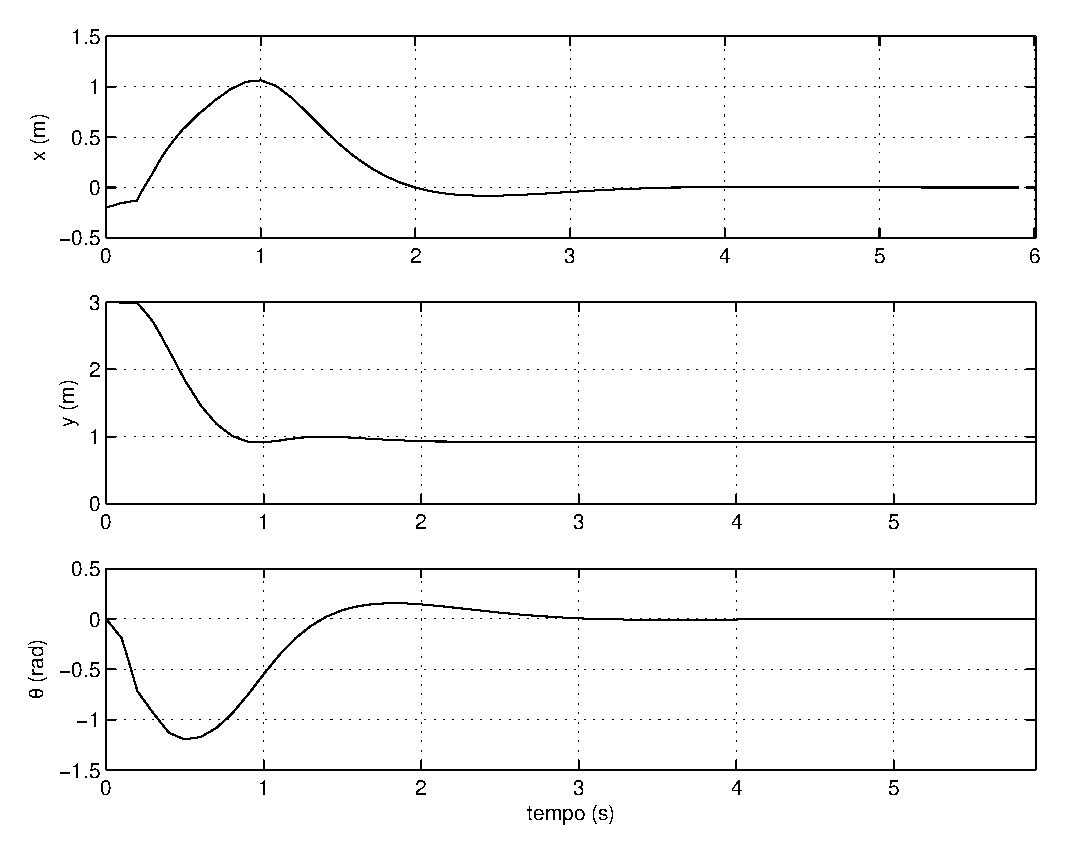
\includegraphics[width=.6\linewidth]{Figuras/pure_mpc/state_01.eps}
    \caption{Estados $x$, $y$ e $\theta$. NMPC com fun��o de custo em coordenadas cartesianas.}
    \label{fig:pure_state_01}
\end{center}\end{figure}

A condi��o final � ${\bf x}_f=[0~~0,91~~0]^T$. Nota-se um grande erro em regime permanente na vari�vel de estado $y$ (Figuras~\ref{fig:pure_traj_01} e \ref{fig:pure_state_01}) (as outras vari�veis convergem para a origem). Uma poss�vel explica��o para este fato � que ambos os estados $x$ e $y$ dependem da velocidade linear $v$. Assim, quando $x$ e $v$ s�o minimizados, a fun��o de custo atinge um valor (uma curva de n�vel da fun��o de custo) que assume ser o seu m�nimo, pelo menos com rela��o a $x$ e $v$. Assim, para minimizar $y$, $v$ e $\Phi$ teriam que aumentar de valor, o que n�o � poss�vel dado ao comportamento monot�nico da fun��o de custo, ou seja, $\Phi(k)\leq\Phi(k-1)$ (Figura~\ref{fig:pure_cost_01}).

\begin{figure}[H]\begin{center}
    \includegraphics[width=.6\linewidth]{Figuras/pure_mpc/control_01.eps}
    \caption{Entradas de controle $v$ e $w$. NMPC com fun��o de custo em coordenadas cartesianas.}
    \label{fig:pure_control_01}
\end{center}\end{figure}
\begin{figure}[H]\begin{center}
    \includegraphics[width=.6\linewidth]{Figuras/pure_mpc/cost_01.eps}
    \caption{Fun��o de custo $\Phi$. NMPC com fun��o de custo em coordenadas cartesianas.}
    \label{fig:pure_cost_01}
\end{center}\end{figure}

Na Figura~\ref{fig:pure_control_01} nota-se que os limite de velocidade, para o rob� Twil, s�o ultrapassados\footnote{Conforme definido no Ap�ndice~\ref{app:twil}, os valores limites para $v$ e $w$ s�o de $\pm 0,4712~m/s$ e $\pm 3,7699~rad/s$, respectivamente.}. Para prevenir isto, restri��es na amplitude dos sinais de controle ser�o consideradas na Se��o~\ref{sec:control_rest}.

O aumento do horizonte de predi��o parece fazer o erro diminuir assintoticamente (Figura~\ref{fig:horizon_effect}). Por outro lado, deseja-se que o horizonte seja o menor poss�vel, j� que o seu tamanho � o principal respons�vel, neste caso, pelo crescimento do custo computacional (vide Se��o~\ref{sec:point_nmpc_cost}).

\begin{figure}[H]\begin{center}
    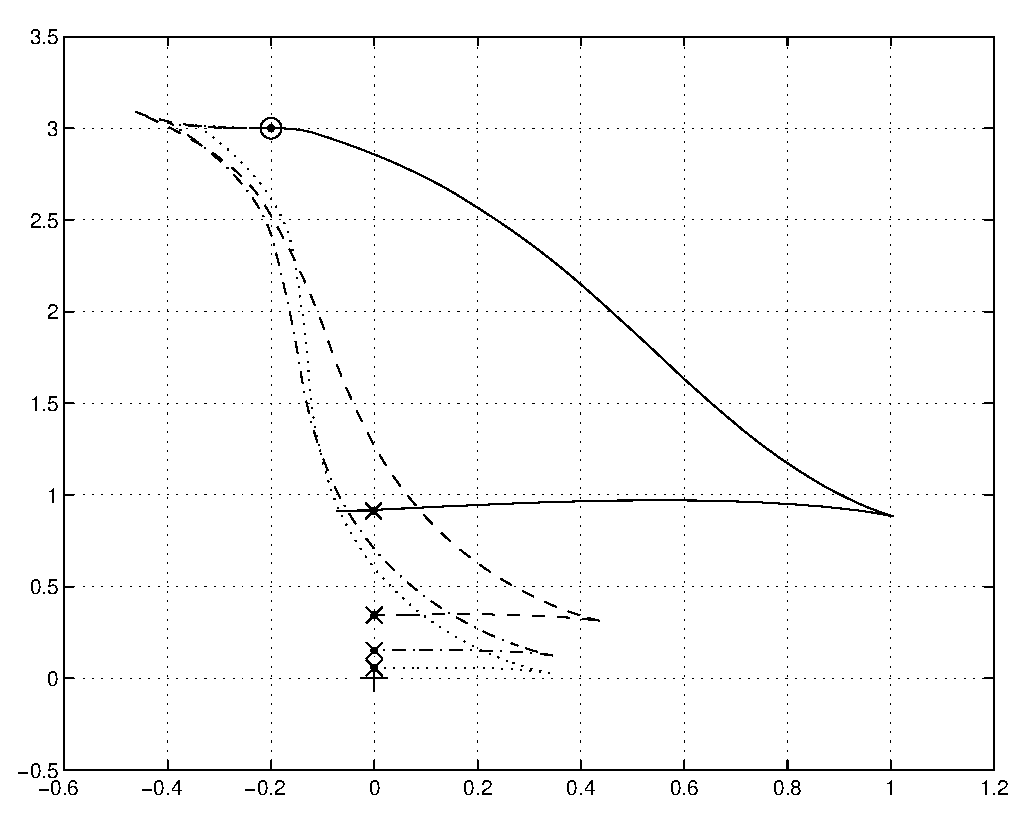
\includegraphics[width=.6\linewidth]{Figuras/pure_mpc/horizon_effect.eps}
    \caption{Efeito do aumento do horizonte $N$ no erro em regime permanente do estado $y$. Linha cont�nua: $N=5$; linha tracejada: $N=10$; linha tra�o-ponto: $N=20$; linha pontilhada: $N=50$.}
    \label{fig:horizon_effect}
\end{center}\end{figure}

Al�m disso, outra alternativa para contornar este problema seria aumentar o peso na vari�vel $y$ atrav�s da matriz $\bf Q$ na fun��o de custo da express�o~\req{eqn:point_cost}. Entretanto, se o ponto de equil�brio tiver sua orienta��o deslocada em $\pi/2$, o problema de erro em regime permanente se transfere para a vari�vel $x$, como pode ser observado pela Figura~\ref{fig:rotated_eq}.

\begin{figure}[H]\begin{center}
    \includegraphics[width=.6\linewidth]{Figuras/pure_mpc/rotated_eq.eps}
    \caption{Trajet�ria no plano $XY$. O ponto de equil�brio � agora ${\bf x}_{ref}=[0~~0~~\pi/2]^T$.}
    \label{fig:rotated_eq}
\end{center}\end{figure}

Os par�metros usados no MPC para o caso acima s�o os mesmos do caso anterior, exceto pela matriz de pondera��o $\bf Q$ e pelo ponto de equil�brio, que agora s�o
\begin{equation*}
	{\bf Q} = \begin{bmatrix} 1 & 0 & 0 \\
						 0 & 50 & 0 \\
						 0 & 0 & 0,5
			\end{bmatrix}, \qquad
	{\bf x}_{ref}= \begin{bmatrix} 0 \\ 0 \\ \pi/2 \end{bmatrix}
\end{equation*}
			
A condi��o final dos estados para o caso apresentado acima � de ${\bf x}_f=[-0,83~~0~~\pi/2]^T$. Observa-se ent�o claramente que o erro em regime permanente antes existente na vari�vel de posi��o $y$ transfere-se para $x$ quando da rota��o do ponto de equil�brio em $\pi/2$, dada a simetria existente entre estas duas vari�veis.

Sendo assim, torna-se necess�ria outra forma de fazer com que todos os estados convirjam para a origem, sem o aumento do horizonte de predi��o.

Ao inv�s da adi��o de uma restri��o terminal, como por exemplo ${\bf x}(k+N|k)=0$ (o que pode tornar o problema de otimiza��o n�o fact�vel), em~\cite{essen01} � proposta uma modifica��o na fun��o de custo a ser minimizada:
\begin{equation}\label{eqn:essen_cost}
	\Phi(k) = \sum_{j=1}^{N-1}{\bf x}^T(k+j|k){\bf Q}(j){\bf x}(k+j|k) + \sum_{j=0}^{N-1}{\bf u}^T(k+j|k){\bf R}{\bf u}(k+j|k) + \Omega({\bf x}(k+N|k)),
\end{equation}
onde a matriz de pondera��o ${\bf Q}(j)$ agora cresce exponencialmente dentro do horizonte e $\Omega({\bf x}(k+N|k))$ � o chamado {\em custo terminal},
\begin{equation*}
	\Omega({\bf x}(k+N|k)) = {\bf x}^T(k+N|k){\bf P}{\bf x}(k+N|k)
\end{equation*}
e ${\bf P}$ � uma matriz tal que aumenta o peso dos estados no final do horizonte, fazendo com que ${\bf x}(k+N|k)$ se aproxime mais da origem. Aqui, escolhe-se
\begin{equation*}
	{\bf Q}(j) = 2^{j-1}{\bf Q}, \quad {\bf P} = 50{\bf Q}(N),
\end{equation*}
e
\begin{equation*}
	{\bf Q} = \begin{bmatrix}	
		1 & 0 & 0 \\
		0 & 1 & 0 \\
		0 & 0 & 0.5 \end{bmatrix}, \quad
	{\bf R} = \begin{bmatrix}
		0.1 & 0 \\ 
		0 & 0.1 \end{bmatrix}
\end{equation*}

Os resultados s�o mostrados abaixo, para uma condi��o inicial do rob� de ${\bf x}_0=[-0,2~~3~~0]^T$.
\begin{figure}[H]\begin{center}
    \includegraphics[width=.6\linewidth]{Figuras/essen_mpc/traj_01.eps}
    \caption{Trajet�ria no plano $XY$. NMPC de \cite{essen01}.}
    \label{fig:essen_traj_01}
\end{center}\end{figure}
\begin{figure}[H]\begin{center}
    \includegraphics[width=.6\linewidth]{Figuras/essen_mpc/state_01.eps}
    \caption{Estados $x$, $y$ e $\theta$. NMPC de \cite{essen01}}
    \label{fig:essen_state_01}
\end{center}\end{figure}
\begin{figure}[H]\begin{center}
    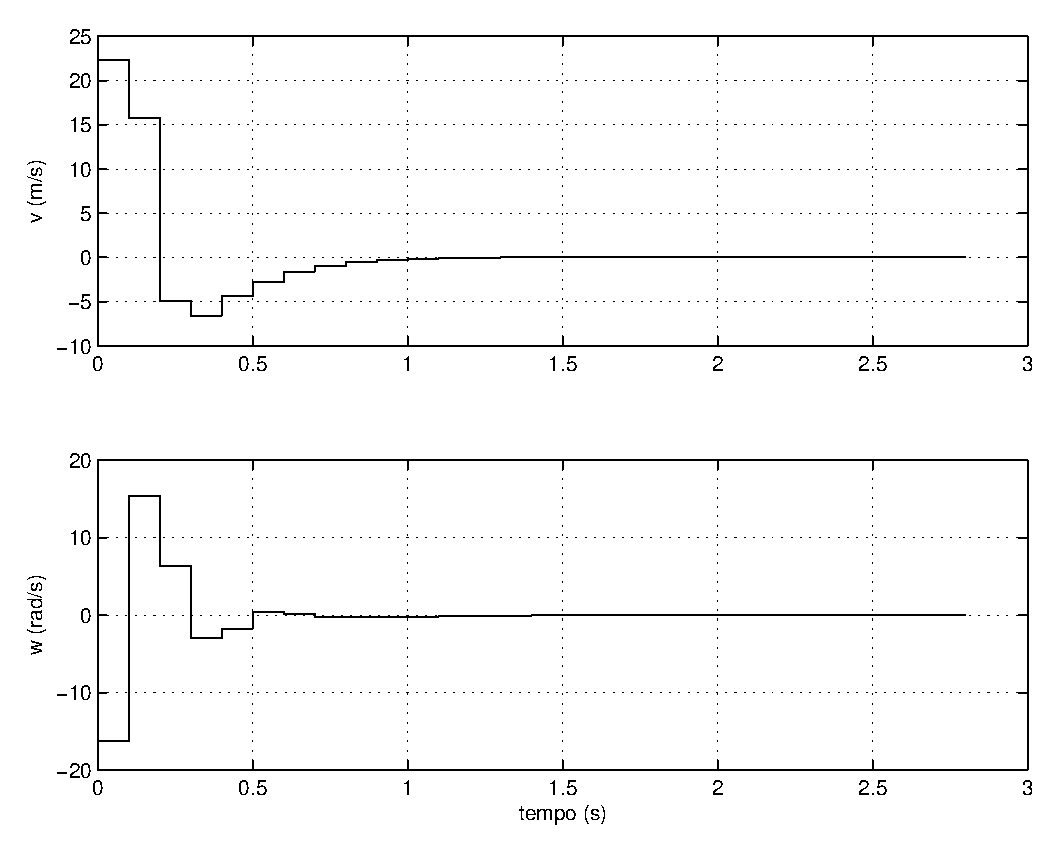
\includegraphics[width=.6\linewidth]{Figuras/essen_mpc/control_01.eps}
    \caption{Entradas de controle $v$ e $w$. NMPC de \cite{essen01}}
    \label{fig:essen_control_01}
\end{center}\end{figure}

A condi��o final agora � de ${\bf x}_f=[0~~-0.003~~0]^T$. Pelos gr�ficos acima, observa-se uma grande diminui��o do erro no estado $y$. Apesar de o esfor�o de controle ter aumentado, o tempo de converg�ncia tamb�m diminuiu bastante. No primeiro caso, o rob� leva cerca de 4 segundos para convergir para a sua configura��o final. Agora, isto acontece em pouco mais de um segundo.

Na Figura~\ref{fig:essen_origin_01} � mostrado um detalhe da origem no plano $XY$. Observa-se que, apesar de o erro em $y$ diminuir, ele n�o � nulo. Nas Figuras~\ref{fig:essen_lots_of_trajs} e~\ref{fig:essen_lots_of_origins}, � mostrado o comportamento do rob� para diversas configura��es iniciais e orienta��o inicial $\theta_0=0~rad$.
\begin{figure}\begin{center}
    \includegraphics[width=.6\linewidth]{Figuras/essen_mpc/origin_01.eps}
    \caption{Detalhe da origem no plano $XY$. NMPC de \cite{essen01}}
    \label{fig:essen_origin_01}
\end{center}\end{figure}
\begin{figure}\begin{center}
    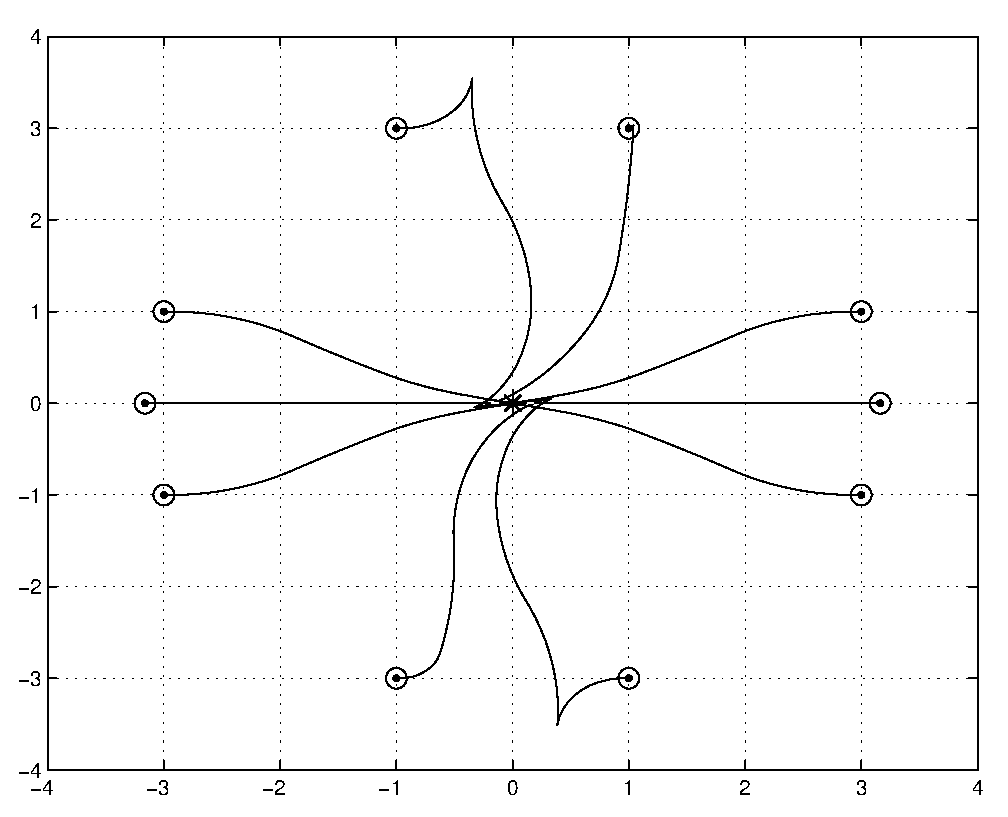
\includegraphics[width=.6\linewidth]{Figuras/essen_mpc/lots_of_trajs.eps}
    \caption{Comportamento do rob� no plano $XY$ para v�rias posi��es de sa�da e $\theta_0=0~rad$. NMPC de \cite{essen01}}
    \label{fig:essen_lots_of_trajs}
\end{center}\end{figure}
\begin{figure}\begin{center}
    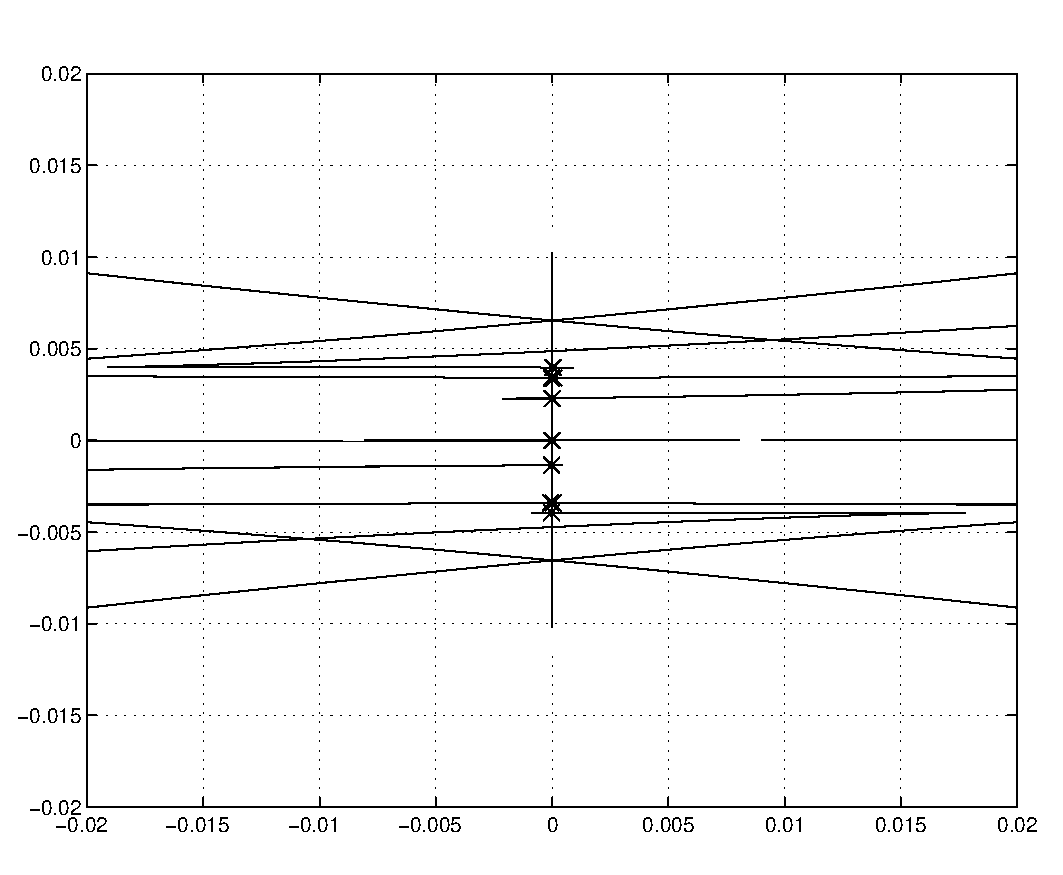
\includegraphics[width=.6\linewidth]{Figuras/essen_mpc/lots_of_origins.eps}
    \caption{Detalhe da origem no plano $XY$ para v�rias posi��es de sa�da e $\theta_0=0~rad$. NMPC de \cite{essen01}}
    \label{fig:essen_lots_of_origins}
\end{center}\end{figure}


%%%%%%%%%%%%%%%%%%%%%%%%%%%%%%%%%%%%%%%%%%%%%%%%%%%%%%%%%%%%%%%%%%%%%%%%%%%
\section{Fun��o de Custo em Coordenadas Polares}\label{sec:point_mpc_polar}
Foi visto que, com as modifica��es apresentadas em \cite{essen01}, � poss�vel diminuir consideravelmente o erro em regime permanente existente em um dos estados de configura��o. Entretanto, um erro de cerca de 0,003~m em $y$ parece ser persistente, pelo menos nos casos apresentados. 

E mais, ainda existe uma simetria entre os estados $x$ e $y$, ambos dependendo da mesma entrada de controle. Para resolver isto, uma transforma��o de coordenadas do modelo cinem�tico do rob� � utilizada. Em~\cite{lages98b}, a seguinte transforma��o descont�nua em coordenadas polares � introduzida (Figura~\ref{fig:polar}):
\begin{align*}
	e      &= \sqrt{x^2+y^2} \\
	\phi   &= \atan(y,x) \\
	\alpha &= \theta - \phi
\end{align*}
e o modelo cinem�tico do rob� nesta base transforma-se em:
\begin{equation}\label{eqn:polar_model}
	\left\{
		\begin{aligned}
			\dot e     &= v\cos\alpha \\
			\dot\phi   &= v\frac{\sen\alpha}{e} \\
			\dot\alpha &= -v\frac{\sen\alpha}{e} + w
		\end{aligned}
	\right.
\end{equation}
onde o vetor de estados � ${\bf x}_p=[e~~\phi~~\alpha]^T$ e ${\bf u}=[v~~w]^T$ s�o as entradas de controle (velocidades linear e angular).
\begin{figure}[hbtp]\begin{center}
    \includegraphics[width=.45\linewidth]{Figuras/polar.eps}
    \caption{Coordenadas polares para o rob� com acionamento diferencial.}
    \label{fig:polar}
\end{center}\end{figure}

\cite{lages98b} prop�e tamb�m a seguinte fun��o de Lyapunov que estabiliza o sistema~\req{eqn:polar_model} na origem:
\begin{equation}\label{eqn:polar_lyapunov}
	V = \frac{1}{2}\left(\lambda e^2 + h\phi^2 + \alpha^2\right),
\end{equation}
onde $\lambda$ e $h$ s�o constantes positivas.	

Esta fun��o de Lyapunov pode ent�o ser utilizada como fun��o de custo~\cite{chen82}. Reescrevendo a express�o \req{eqn:polar_lyapunov} em uma forma quadr�tica,
\begin{equation*}
	V = {\bf x}_p^T{\bf Q}_p{\bf x}_p, \qquad {\bf Q}_p = \begin{bmatrix}
		\frac{1}{2}\lambda & 0 & 0 \\
		0 & \frac{1}{2}h & 0 \\
		0 & 0 & \frac{1}{2}
	\end{bmatrix}
\end{equation*}
e incluindo um termo de penaliza��o do controle, tem-se a seguinte fun��o de custo para o sistema em coordenadas polares:
\begin{equation}\label{eqn:polar_cost}
	\Phi_p(k) = \sum_{j=1}^{N}{\bf x}_p^T(k+j|k){\bf Q}_p{\bf x}_p(k+j|k) + {\bf u}^T(k+j-1|k){\bf R}{\bf u}(k+j-1|k)
\end{equation}

considera-se ent�o o seguinte problema de NMPC:
\begin{equation*}
{\bf u}^\star,~{\bf x}^\star = \arg\min_{{\bf u},{\bf x}}\left\{\Phi_p(k)\right\}
\end{equation*}
sujeito �:
\begin{align*}
	{\bf x}(k|k)   &= {\bf x}_0, \\
	{\bf x}(k+j|k) &= f({\bf x}(k+j-1|k),{\bf u}(k+j-1|k)), \quad j\in[1,N]
\end{align*}
e com os seguintes par�metros:
\begin{equation*}
	N=5, \quad \lambda=2, \quad h=2, \quad {\bf R} = \begin{bmatrix}
		0.1 & 0 \\ 
		0 & 0.1 \end{bmatrix},
\end{equation*}
obtendo-se os resultados que seguem, para uma condi��o inicial de ${\bf x}_0=[-0.2~~3~~0]^T$:
\begin{figure}[H]\begin{center}
    \includegraphics[width=.6\linewidth]{Figuras/polar_mpc/traj_01.eps}
    \caption{Trajet�ria no plano $XY$. NMPC com fun��o de custo em coordenadas polares.}
    \label{fig:polar_traj_01}
\end{center}\end{figure}
\begin{figure}[H]\begin{center}
    \includegraphics[width=.6\linewidth]{Figuras/polar_mpc/state_01.eps}
    \caption{Estados $x$, $y$ e $\theta$. NMPC com fun��o de custo em coordenadas polares.}
    \label{fig:polar_state_01}
\end{center}\end{figure}
\begin{figure}\begin{center}
    \includegraphics[width=.6\linewidth]{Figuras/polar_mpc/control_01.eps}
    \caption{Entradas de controle $v$ e $w$. NMPC com fun��o de custo em coordenadas polares.}
    \label{fig:polar_control_01}
\end{center}\end{figure}
\begin{figure}\begin{center}
    \includegraphics[width=.6\linewidth]{Figuras/polar_mpc/cost_01.eps}
    \caption{Fun��o de custo $\Phi$. NMPC com fun��o de custo em coordenadas polares.}
    \label{fig:polar_cost_01}
\end{center}\end{figure}
\begin{figure}\begin{center}
    \includegraphics[width=.6\linewidth]{Figuras/polar_mpc/origin_01.eps}
    \caption{Detalhe na origem do plano $XY$. NMPC com fun��o de custo em coordenadas polares.}
    \label{fig:polar_origin_01}
\end{center}\end{figure}

Ent�o, observa-se que, com a transforma��o em coordenadas polares na fun��o de custo, sem aumentar o horizonte de predi��o e sem adi��o de outros termos, todos os estados convergem assintoticamente para a origem, sem apresentar erro em regime permanente. Neste caso, o rob� estabiliza exatamente na origem.

O motivo pelo qual o uso de uma fun��o de custo em coordenadas polares resolve o problema apresentado no in�cio deste cap�tulo ainda est� em estudo. Entretanto, com base nos resultados, pode-se conjecturar o seguinte:
\begin{itemize}
\item Em~\cite{lages98b} � visto que a converg�ncia de um dos estados em coordenadas polares para zero faz com que todas as outras vari�veis de estado tamb�m convirgam para zero. Assim, uma poss�vel proposi��o � que esta propriedade tamb�m se estende para o caso do NMPC apresentado aqui;
\item Com uma fun��o de custo em coordenadas cartesianas, devido �s restri��es referentes ao modelo do sistema, o ponto �timo encontrado pelo algoritmo de otimiza��o n�o � �nico, fazendo com que o valor da fun��o de custo fique preso em alguma curva de n�vel n�o nula. Com a mudan�a de base da fun��o de custo para coordenadas polares, a estrutura da fun��o de custo � modificada e provavelmente este problema � eliminado.
\end{itemize}


%%%%%%%%%%%%%%%%%%%%%%%%%%%%%%%%%%%%%%%%%%%%%%%%%%%%%%%%%%%%%%%%
\section{MPC com Restri��es no Controle}\label{sec:control_rest}
At� aqui, a �nica restri��o imposta no problema de otimiza��o foi aquela referente � din�mica do modelo cinem�tico do rob�. Nesta se��o, ser�o inseridos limites nas amplitudes das entradas de controle, a serem respeitados durante a minimiza��o da fun��o de custo. Levando em conta as caracter�sticas do rob� Twil, definidas no Ap�ndice~\ref{app:twil}, pode-se formular as seguintes restri��es nas amplitudes das velocidades linear e angular:
\begin{alignat*}{3}
	-\overline v &\leq &v &\leq \overline v, &\quad \overline v &= 0,4712~m/s \\ 
	-\overline w &\leq &w &\leq \overline w, &\quad \overline w &= 3,7699~rad/s
\end{alignat*}

Fazendo ${\bf u}=[v~~w]^T$, tem-se que $-\overline{\bf u}\leq{\bf u}\leq\overline{\bf u}$. Esta restri��o pode ser reescrita na forma da desigualdade ${\bf Du}\leq{\bf d}$ (express�o~\req{eqn:restu}) com:
\begin{equation}\label{eqn:mtx_restu}
	{\bf D} = \begin{bmatrix}
		\bf I \\ -\bf I
	\end{bmatrix} \quad \text{e}\quad {\bf d}= \begin{bmatrix}
		\overline{\bf u} \\ \overline{\bf u}
	\end{bmatrix},
\end{equation}
ou seja,
\begin{equation*}
	\begin{bmatrix}
		1 & 0 \\ 0 & 1 \\ -1 & 0 \\ 0 & -1
	\end{bmatrix}	\begin{bmatrix} v \\ w 
	\end{bmatrix} \leq \begin{bmatrix}
		0,4712~m/s \\ 3,7699~rad/s \\ 0,4712~m/s \\ 3,7699~rad/s
	\end{bmatrix}
\end{equation*}

Assim, tem-se o seguinte problema de otimiza��o para o rob�, utilizando a fun��o de custo~\req{eqn:polar_cost} em coordenadas polares:
\begin{equation*}
	{\bf u}^\star,~{\bf x}^\star = \arg\min_{{\bf u},{\bf x}}\left\{\Phi_p(k)\right\}
\end{equation*}
sujeito �:
\begin{alignat*}{2}
	{\bf x}(k|k)	 &= {\bf x}_0, \\
	{\bf x}(k+j|k)  &= f({\bf x}(k+j-1|k),{\bf u}(k+j-1|k)), &~~~ j&\in[1,N] \\
	{\bf Du}(k+j|k) &\leq {\bf d}, &~~~ j&\in[0,N-1]
\end{alignat*}
com $\bf D$ e $\bf d$ definidos pela express�o~\req{eqn:mtx_restu}. Com os seguintes par�metros de sintonia:
\begin{equation*}
	N=5, \quad \lambda=2, \quad h=2, \quad {\bf R} = \begin{bmatrix}
		0.1 & 0 \\ 
		0 & 0.1 \end{bmatrix},
\end{equation*}
obt�m-se ent�o os seguintes resultados, para uma condi��o inicial de ${\bf x}_0=[-0.2~~3~~0]^T$:
\begin{figure}[H]\begin{center}
    \includegraphics[width=.6\linewidth]{Figuras/restu_mpc/traj_01.eps}
    \caption{Trajet�ria no plano $XY$. NMPC com fun��o de custo em coordenadas polares.}
    \label{fig:restu_traj_01}
\end{center}\end{figure}
\begin{figure}[H]\begin{center}
    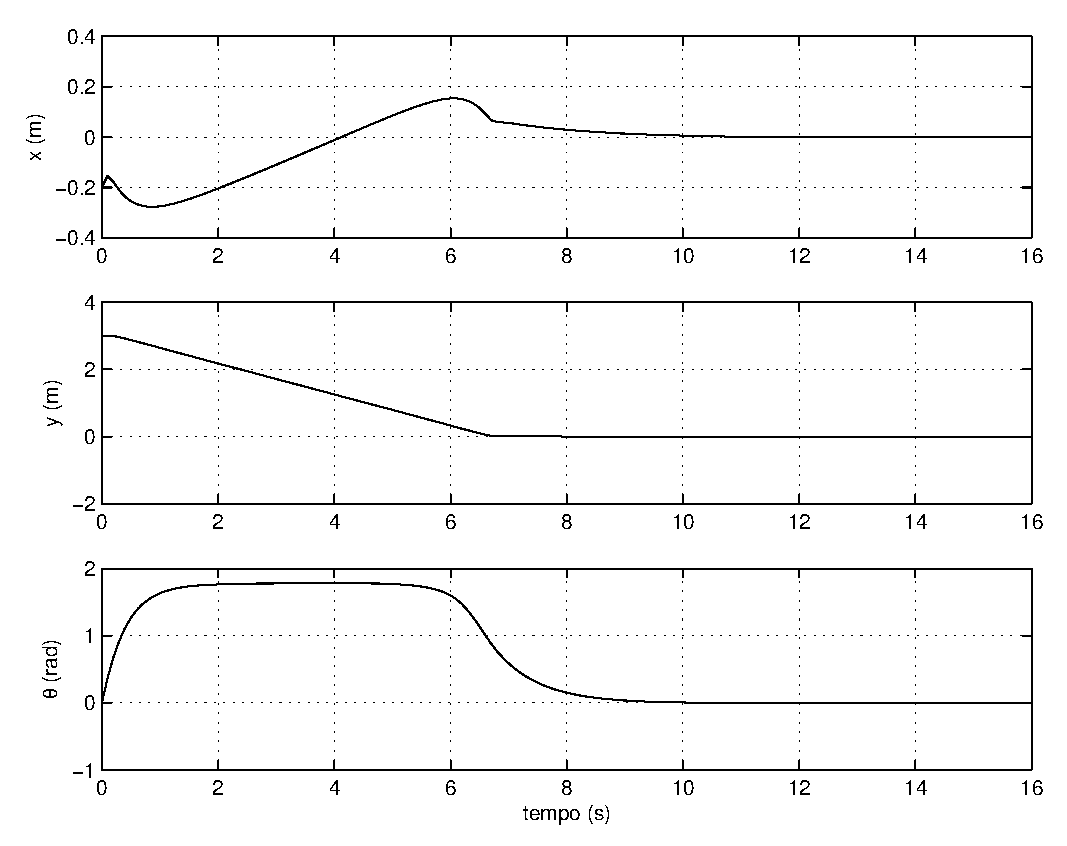
\includegraphics[width=.6\linewidth]{Figuras/restu_mpc/state_01.eps}
    \caption{Estados $x$, $y$ e $\theta$. NMPC com fun��o de custo em coordenadas polares.}
    \label{fig:restu_state_01}
\end{center}\end{figure}

O ponto mais importante a ser ressaltado aqui � o de que a fun��o de custo foi minimizada respeitando-se as restri��es de amplitude das entradas de controle impostas pela express�o~\req{eqn:mtx_restu} nas velocidades linear e angular, o que pode ser claramente observado no gr�fico da Figura~\ref{fig:restu_control_01}.

Obviamente que, por causa destas restri��es, as velocidades desenvolvidas est�o muito abaixo das apresentadas nos casos anteriores, e por isso o rob� demora um tempo maior para chegar ao seu objetivo. Por exemplo, no caso sem restri��es da Figura~\ref{fig:polar_state_01} observa-se que o rob� chega � origem em cerca de 4 segundos, o que agora acontece em pelo menos o dobro desse tempo.

\begin{figure}[H]\begin{center}
    \includegraphics[width=.6\linewidth]{Figuras/restu_mpc/control_01.eps}
    \caption{Entradas de controle $v$ e $w$. NMPC com fun��o de custo em coordenadas polares.}
    \label{fig:restu_control_01}
\end{center}\end{figure}
\begin{figure}[H]\begin{center}
    \includegraphics[width=.6\linewidth]{Figuras/restu_mpc/cost_01.eps}
    \caption{Fun��o de custo $\Phi$. NMPC com fun��o de custo em coordenadas polares.}
    \label{fig:restu_cost_01}
\end{center}\end{figure}

A seguir, � feita uma compara��o entre este �ltimo caso, com a fun��o de custo em coordenadas polares da express�o~\req{eqn:polar_cost}, o caso do NMPC de~\cite{essen01} (fun��o de custo da espress�o~\req{eqn:essen_cost}) e o caso com a fun��o de custo original, em coordenadas cartesianas da express�o~\req{eqn:point_cost}, sem a adi��o do custo terminal e com uma matriz $\bf Q$ constante. Os resultados de cada caso s�o representados, nos gr�ficos das Figuras~\ref{fig:restu_traj_02} e \ref{fig:restu_state_02}, pelas linhas cont�nuas e tracejadas e tra�o-ponto, respectivamente. A matriz $\bf Q$ (${\bf Q}={\rm diag}(1;1;0,5)$) e todos os par�metros de sintonia s�o os mesmos para os tr�s casos. A condi��o inicial do rob� � ${\bf x}_0=[3~~6~~0]^T$. 
\begin{figure}[H]\begin{center}
    \includegraphics[width=.6\linewidth]{Figuras/restu_mpc/traj_02.eps}
    \caption{Trajet�ria no plano $XY$. Linha cont�nua: NMPC com fun��o de custo em coordenadas polares; linha tracejada: NMPC de~\cite{essen01}; linha tra�o-ponto: NMPC com fun��o de custo em coordenadas cartesianas.}
    \label{fig:restu_traj_02}
\end{center}\end{figure}
\begin{figure}[H]\begin{center}
    \includegraphics[width=.6\linewidth]{Figuras/restu_mpc/state_02.eps}
    \caption{Estados $x$, $y$ e $\theta$. Linha cont�nua: NMPC com fun��o de custo em coordenadas polares; linha tracejada: NMPC de~\cite{essen01}; linha tra�o-ponto: NMPC com fun��o de custo em coordenadas cartesianas.}
    \label{fig:restu_state_02}
\end{center}\end{figure}

Observa-se ent�o que existe um grande erro na vari�vel $y$ quando se usa a fun��o de custo original, fato j� constatado nos primeiros casos apresentados neste cap�tulo. A condi��o final para o NMPC com fun��o de custo em coordenadas polares � ${\bf x}_0=[0~~0~~0]^T$, ${\bf x}_0=[0~~0,003~~0]^T$ para o NMPC de~\cite{essen01} e de ${\bf x}_0=[-0,0022~~1,4407~~0,0014]^T$ para o NMPC com fun��o de custo original. Ainda, a Figura~\ref{fig:restu_control_02} mostra que o esfor�o de controle � bem menor quando a fun��o de custo � escrita em coordenadas polares. Todos os casos respeitam os limites impostos (Figura~\ref{fig:restu_control_02}), mesmo com uma condi��o inicial relativamente longe da origem, se comparado com os casos anteriores.
\begin{figure}[H]\begin{center}
    \includegraphics[width=.6\linewidth]{Figuras/restu_mpc/control_02.eps}
    \caption{Entradas de controle $v$ e $w$. Linha cont�nua: NMPC com fun��o de custo em coordenadas polares; linha tracejada: NMPC de~\cite{essen01}; linha tra�o-ponto: NMPC com fun��o de custo em coordenadas cartesianas.}
    \label{fig:restu_control_02}
\end{center}\end{figure}
\begin{figure}[H]\begin{center}
    \includegraphics[width=.6\linewidth]{Figuras/restu_mpc/cost_02.eps}
    \caption{Fun��o de custo $\Phi$. Linha cont�nua: NMPC com fun��o de custo em coordenadas polares; linha tracejada: NMPC de~\cite{essen01}; linha tra�o-ponto: NMPC com fun��o de custo em coordenadas cartesianas.}
    \label{fig:restu_cost_02}
\end{center}\end{figure}

%%%%%%%%%%%%%%%%%%%%%%%%%%%%%%%%%%%%%%%%%%%%%%%%%%%%%%%%%%%%%%%%%%%%%%%%%%%%%%%%%%
\section{MPC Com Restri��es no Controle e no Estado}\label{sec:control_state_rest}
Nesta se��o ser� mostrado um exemplo ilustrativo onde o objetivo � fazer com que o rob� cruze um corredor sem tocar nas paredes. A exist�ncia de restri��es de amplitude nas entradas de controle e nas vari�veis de estado � ent�o considerada. Assim, na Figura~\ref{fig:corridor_corridor} tem-se o espa�o de configura��o, no plano $XY$, no qual est� inserido o rob�.
\begin{figure}\begin{center}
    \includegraphics[width=.6\linewidth]{Figuras/corridor_mpc/corridor.eps}
    \caption{Espa�o de configura��o no plano $XY$: um corredor em "L".}
    \label{fig:corridor_corridor}
\end{center}\end{figure}

Os pol�gonos cinzas indicam a exist�ncia de paredes, ou seja, pontos onde o rob� � impedido de cruzar. 

De uma forma geral, a seguinte restri��o na amplitude dos estados � formulada:
\begin{equation*}
	{\bf x}(k+j|k)\in\mathbb{X}, \quad j\in[0,N],
\end{equation*}
onde $\mathbb{X}$ � um conjunto convexo de poss�veis estados e cont�m o ponto de equil�brio em seu interior~\cite{mayne00}. Entretanto, nota-se na Figura~\ref{fig:corridor_corridor} que a regi�o de configura��o no plano $XY$ n�o � mais convexa, dada a exist�ncia das paredes do corredor.

Para que o problema de otimiza��o utilizado aqui possa ser resolvido, as restri��es sobre os estados  de configura��o precisam ser convexas. Isto pode ser feito atrav�s da divis�o da regi�o de configura��o em diferentes semi-espa�os,  aplicando ent�o uma estrat�gia de {\em pontos de passagem}, ou seja, dependendo da posi��o do rob� um conjunto diferente de restri��es convexas � considerado no problema de otimiza��o. Considera-se ainda um ponto de refer�ncia diferente para cada uma destes semi-espa�os. Assim, problemas de otimiza��o diferentes s�o resolvidos, dependendo da posi��o inicial onde que se encontra o rob�.

Para a regi�o apresentada na Figura~\ref{fig:corridor_corridor}, considera-se a exist�ncia de dois sub-espa�os
$\mathbb{H}_1$ e $\mathbb{H}_2$ com fronteira determinada pela reta $x=-1$:
\begin{align*}
	\mathbb{H}_1=\{{\bf x}(k+j|k)\in\real;~~x(k|k)<-1\}, \\
	\mathbb{H}_2=\{{\bf x}(k+j|k)\in\real;~~x(k|k)\geq-1\}
\end{align*}

Assim, dentro de cada um desses sub-espa�os, definem-se as sub-regi�es $\mathbb{X}_1\subseteq\mathbb{X}$ e $\mathbb{X}_2\subseteq\mathbb{X}$ tais que:
\begin{equation*}
	\mathbb{X} = \mathbb{X}_1 \cup \mathbb{X}_2
\end{equation*}

Como dito, a fronteira entre estas sub-regi�es � $x=-1$, ou seja,
\begin{align*}
	{\bf x}\in \mathbb{X}_1, \quad \text{se}~~x(k|k)<-1, \\
	{\bf x}\in \mathbb{X}_2, \quad \text{se}~~x(k|k)\geq-1,
\end{align*}
ou, reescrevendo na forma da desigualdade~\req{eqn:restx},
\begin{align}
	{\bf Cx} &\leq {\bf c}_1, \quad \text{se}~~x(k|k)<-1, \label{eqn:ineq1} \\
	{\bf Cx} &\leq {\bf c}_2, \quad \text{se}~~x(k|k)\geq-1 \label{eqn:ineq2}
\end{align}
e os pontos de equil�brio em $\mathbb{X}_1$ e $\mathbb{X}_2$ s�o, respectivamente,
\begin{equation*}
	{\bf x}_{ref,1}=\begin{bmatrix}0\\4\\0\end{bmatrix}, \quad{\text e}\quad
	{\bf x}_{ref,2}=\begin{bmatrix}0\\0\\0\end{bmatrix}
\end{equation*}

No caso considerado, tem-se que:
\begin{align}
	\mathbb{X}_1 &= \{{\bf x}~|~x(k+j|k)\leq -1; 3\leq y(k+j|k)\leq 5\}  \label{eqn:subreg_1}\\
	\mathbb{X}_2 &= \{{\bf x}~|~-1\leq x(k+j|k)\leq 1; y(k+j|k)\leq 5\} \label{eqn:subreg_2}
\end{align}
ent�o, $\bf C$, ${\bf c}_1$ e ${\bf c}_2$ em \req{eqn:ineq1} e \req{eqn:ineq2} s�o
\begin{equation*}
	{\bf C}=\begin{bmatrix} {\bf I}\\-{\bf I} \end{bmatrix}, \qquad
	{\bf c}_1 = \begin{bmatrix}-1\\5\\\infty\\\infty\\-3\\\infty\end{bmatrix}, \qquad
	{\bf c}_2 = \begin{bmatrix}1\\5\\\infty\\1\\\infty\\\infty\end{bmatrix},
\end{equation*}
onde $\infty$ indica que a vari�vel correspondente n�o possui restri��o.

Assim, enquanto o rob� estiver se movimentando dentro do semi-espa�o H1, as restri��es a serem consideradas 
sobre os estados ser�o dadas por $\mathbb{X}_1$, o seu objetivo ser� estabilizar em ${\bf x}_{ref,1}$ respeitando as restri��es de estado referentes � express�o~\req{eqn:subreg_1}. Atingido um ponto pertencente ao semi-espa�o H2, as restri��es sobre os estados passam a ser descritas por  $\mathbb{X}_2$, o objetivo ser� ent�o estabilizar na origem respeitando-se as restri��es referentes � express�o~\req{eqn:subreg_2}. 

%Isto pode ser solucionado se o problema for tratado de forma {\em multi-objetiva}, ou seja, separa-se o conjunto $\mathbb X$ em subregi�es de forma que estas subregi�es sejam convexas e contenham um ponto de equil�brio em seu interior. Neste caso, definem-se $\mathbb{X}_1\subseteq\mathbb{X}$ e $\mathbb{X}_2\subseteq\mathbb{X}$ tal que:
%\begin{equation*}
%	\mathbb{X} = \mathbb{X}_1 \cup \mathbb{X}_2
%\end{equation*}

%No caso considerado, tem-se que:
%\begin{align}
%	\mathbb{X}_1 &= \{{\bf x}~|~x\leq -1; 3\leq y\leq 5\}  \label{eqn:subreg_1}\\
%	\mathbb{X}_2 &= \{{\bf x}~|~-1\leq x\leq 1; y\leq 5\} \label{eqn:subreg_2}
%\end{align}

%Os pontos de equil�brio em $\mathbb{X}_1$ e $\mathbb{X}_2$ s�o, respectivamente,
%\begin{equation*}
%	{\bf x}_{ref,1}=\begin{bmatrix}0\\4\\0\end{bmatrix}, \quad{\text e}\quad
%	{\bf x}_{ref,2}=\begin{bmatrix}0\\0\\0\end{bmatrix}
%\end{equation*}

%Assim, enquanto o rob� estiver se movimentando dentro da regi�o pertencente a $\mathbb{X}_1$, o seu objetivo ser� estabilizar em ${\bf x}_{ref,1}$ respeitando as restri��es de estado referentes � express�o~\req{eqn:subreg_1}. Atingido um ponto pertencente � regi�o $\mathbb{X}_2$, o objetivo ser� ent�o estabilizar na origem respeitando-se as restri��es referentes � express�o~\req{eqn:subreg_2}. Neste caso, adotou-se $x=-1$ como fronteira entre as duas subregi�es, ou seja,
%\begin{align*}
%	{\bf x}\in \mathbb{X}_1, \quad \text{se}~~x<-1, \\
%	{\bf x}\in \mathbb{X}_2, \quad \text{se}~~x\geq-1,
%\end{align*}
%ou, reescrevendo na forma da desigualdade~\req{eqn:restx},
%\begin{align*}
%	{\bf Cx} &\leq {\bf c}_1, \quad \text{se}~~x<-1, \\
%	{\bf Cx} &\leq {\bf c}_2, \quad \text{se}~~x\geq-1
%\end{align*}
%com
%\begin{equation*}
%	{\bf C}=\begin{bmatrix} {\bf I}\\-{\bf I} \end{bmatrix}, \qquad
%	{\bf c}_1 = \begin{bmatrix}-1\\5\\\infty\\\infty\\-3\\\infty\end{bmatrix}, \qquad
%	{\bf c}_2 = \begin{bmatrix}1\\5\\\infty\\1\\\infty\\\infty\end{bmatrix},
%\end{equation*}
%onde $\infty$ indica que a vari�vel correspondente n�o possui restri��o.	

Assim, o MPC, para este caso, � resolvido da seguinte maneira, para cada instante de amostragem $k$:
\begin{equation*}
	{\bf u}^\star,~{\bf x}^\star = \arg\min_{{\bf u},{\bf x}}\left\{\Phi_p(k)\right\}
\end{equation*}
sujeito �:
\begin{alignat*}{2}
	{\bf x}(k|k)	 &= {\bf x}_0, \\
	{\bf x}(k+j|k)  &= f({\bf x}(k+j-1|k),{\bf u}(k+j-1|k)), &\quad j &\in[1,N] \notag \\
	{\bf Cx}(k+j|k) &\leq {\bf c}_1, \quad \text{se }~~x(k|k)<-1, &\quad j &\in[0,N] \\
	{\bf Cx}(k+j|k) &\leq {\bf c}_2, \quad \text{se }~~x(k|k)\geq-1, &\quad j &\in[0,N] \\
	{\bf Du}(k+j|k) &\leq {\bf d},   &\quad j &\in[0,N-1]
\end{alignat*}
com a seguinte fun��o de custo:
\begin{equation*}
	\Phi_p(k) = \sum_{j=1}^{N}\tilde{\bf x}_p^T(k+j|k){\bf Q}_p\tilde{\bf x}_p(k+j|k) + {\bf u}^T(k+j-1|k){\bf R}{\bf u}(k+j-1|k),
\end{equation*}
onde
\begin{equation*}
	\tilde{\bf x}_p=\begin{bmatrix}
		\tilde e\\\tilde\phi\\\tilde\alpha
	\end{bmatrix} = \begin{bmatrix}
		\sqrt{(x-x_{ref,i})^2+(y-y_{ref,i})^2} \\
		\atan(y-y_{ref,i},x-x_{ref,i}) \\
		\theta-\theta_{ref,i}-\phi
	\end{bmatrix}, \quad i=1,2
\end{equation*}			

Ent�o, com
\begin{equation*}
	N=5, \quad \lambda=2, \quad h=2, \quad {\bf R} = \begin{bmatrix}
		0.1 & 0 \\ 
		0 & 0.1 \end{bmatrix},
\end{equation*}
obt�m-se os seguintes resultados, para um condi��o inicial de ${\bf x}_0=[-4~~4~~\pi]^T$:
\begin{figure}[H]\begin{center}
    \includegraphics[width=.6\linewidth]{Figuras/corridor_mpc/traj_01.eps}
    \caption{Trajet�ria no plano $XY$. NMPC com fun��o de custo em coordenadas polares.}
    \label{fig:corridor_traj_01}
\end{center}\end{figure}
\begin{figure}[H]\begin{center}
    \includegraphics[width=.6\linewidth]{Figuras/corridor_mpc/state_01.eps}
    \caption{Estados $x$, $y$ e $\theta$. NMPC com fun��o de custo em coordenadas polares.}
    \label{fig:corridor_state_01}
\end{center}\end{figure}
\begin{figure}\begin{center}
    \includegraphics[width=.6\linewidth]{Figuras/corridor_mpc/control_01.eps}
    \caption{Entradas de controle $v$ e $w$. NMPC com fun��o de custo em coordenadas polares.}
    \label{fig:corridor_control_01}
\end{center}\end{figure}
\begin{figure}\begin{center}
    \includegraphics[width=.6\linewidth]{Figuras/corridor_mpc/cost_01.eps}
    \caption{Fun��o de custo $\Phi$. NMPC com fun��o de custo em coordenadas polares.}
    \label{fig:corridor_cost_01}
\end{center}\end{figure}

Nota-se ent�o pelas Figuras~\ref{fig:corridor_traj_01} a \ref{fig:corridor_cost_01} que o resultado � bastante satisfat�rio. A condi��o final � do rob� ${\bf x}_f=[0~~0~~0]^T$. o movimento do rob� � bastante suave e o choque com as paredes do corredor � evitado com sucesso. As restri��es de amplitude das entradas de controle s�o respeitadas. Observa-se tamb�m na Figura~\ref{fig:corridor_cost_01} que, como o ponto ao qual o rob� deve convergir muda durante o percorrer da trajet�ria, a fun��o de custo n�o � monotonicamente decrescente.

Agora, da Figura~\ref{fig:corridor_traj_comp}, observa-se que, se n�o existissem as restri��es nos estados $x$ e $y$, o rob� iria de encontro � parede (linha tracejada do gr�fico), provocando seu choque com a mesma.
\begin{figure}\begin{center}
    \includegraphics[width=.6\linewidth]{Figuras/corridor_mpc/traj_comp.eps}
    \caption{Trajet�ria no plano $XY$. NMPC com fun��o de custo em coordenadas polares. Linha cont�nua: com restri��es nos estados; Linha tracejada: sem restri��es nos estados.}
    \label{fig:corridor_traj_comp}
\end{center}\end{figure}

E na Figura~\ref{fig:corridor_traj_02} � mostrado um caso semelhante ao anterior, mas agora com o corredor invertido em rela��o ao eixo $Y$ e com condi��o inicial em ${\bf x}_0=[4~~4.3~~\pi]^T$.
\begin{figure}[H]\begin{center}
    \includegraphics[width=.6\linewidth]{Figuras/corridor_mpc/traj_02.eps}
    \caption{Trajet�ria no plano $XY$. NMPC com fun��o de custo em coordenadas polares.}
    \label{fig:corridor_traj_02}
\end{center}\end{figure}
%\begin{figure}[H]\begin{center}
%    \includegraphics[width=.6\linewidth]{Figuras/corridor_mpc/state_02.eps}
%    \caption{Estados $x$, $y$ e $\theta$. NMPC com fun��o de custo em coordenadas polares.}
%    \label{fig:corridor_state_02}
%\end{center}\end{figure}
%\begin{figure}[H]\begin{center}
%    \includegraphics[width=.6\linewidth]{Figuras/corridor_mpc/control_02.eps}
%    \caption{Entradas de controle $v$ e $w$. NMPC com fun��o de custo em coordenadas polares.}
%    \label{fig:corridor_control_02}
%\end{center}\end{figure}
%\begin{figure}[H]\begin{center}
%    \includegraphics[width=.6\linewidth]{Figuras/corridor_mpc/cost_02.eps}
%    \caption{Fun��o de custo $\Phi$. NMPC com fun��o de custo em coordenadas polares.}
%    \label{fig:corridor_cost_02}
%\end{center}\end{figure}


%%%%%%%%%%%%%%%%%%%%%%%%%%%%%%%%%%%%%%%%%%%%%%%%%%%%%
\section{An�lises Comparativas}\label{sec:point_comp}
Nesta se��o v�rias an�lises comparativas ser�o mostradas. Primeiramente as duas t�cnicas de NMPC desenvolvidas durante este cap�tulo ser�o mostradas, e ap�s as compara��es ser�o feitas entre o NMPC com fun��o de custo em coordenadas polares e com restri��o de amplitude nas entradas de controle e as leis de controle variantes no tempo e n�o suaves apresentadas das Se��es~\ref{sec:timevar} e \ref{sec:disc}.

Dentro desta se��o, a restri��o nas entradas de controle da express�o~\req{eqn:mtx_restu} � considerada e os seguintes par�metros s�o utilizados no NMPC com fun��o de custo em coordenadas polares: $\lambda=2$, $h=2$, $N = 5$ e
\begin{equation*}
	{\bf R} = \begin{bmatrix} 0.1 & 0 \\ 0 & 0.1 \end{bmatrix}
\end{equation*}


%%%%%%%%%%%%%%%%%%%%%%%%%%%%%%%%%%%%%%%%%%%%%%%%%%%%%%%%%%%%%%%%%%%%%%%%%%%%%%%%%%%%%%%%%%%%%%%%%%%%%%%%%%
\subsection{Compara��o Entre o NMPC Com Fun��o De Custo Em Coordenadas Polares e o NMPC de~\cite{essen01}}
Para o NMPC de~\cite{essen01}, definido na Se��o~\ref{sec:cart}, os par�metros utilizados s�o os seguintes: $N=5$, ${\bf Q}(j)=2^{j-1}{\bf Q}$, ${\bf P}=50{\bf Q}(N)$ e
\begin{equation*}
	{\bf Q} = \begin{bmatrix}	
		1 & 0 & 0 \\
		0 & 1 & 0 \\
		0 & 0 & 0.5 \end{bmatrix}, \quad
		{\bf R} = \begin{bmatrix} 0.1 & 0 \\ 0 & 0.1 \end{bmatrix}
\end{equation*}
e para ambos os casos, restri��es nas entradas de controle conforme a express�o~\req{eqn:mtx_restu} s�o consideradas.

Os resultados s�o mostrados abaixo para uma condi��o inicial de ${\bf x}_0=[-2~~2~~\pi/2]^T$.
\begin{figure}[H]\begin{center}
    \includegraphics[width=.6\linewidth]{Figuras/comps/traj_01.eps}
    \caption{Trajet�ria no plano $XY$. Linha cont�nua: NMPC com fun��o de custo em coordenadas polares; Linha tracejada: NMPC de~\cite{essen01}.}
    \label{fig:comps_traj_01}
\end{center}\end{figure}
\begin{figure}[H]\begin{center}
    \includegraphics[width=.6\linewidth]{Figuras/comps/state_01.eps}
    \caption{Estados $x$, $y$ e $\theta$. Linha cont�nua: NMPC com fun��o de custo em coordenadas polares; Linha tracejada: NMPC de~\cite{essen01}.}
    \label{fig:comps_state_01}
\end{center}\end{figure}
\begin{figure}\begin{center}
    \includegraphics[width=.6\linewidth]{Figuras/comps/control_01.eps}
    \caption{Entradas de controle $v$ e $w$. Linha cont�nua: NMPC com fun��o de custo em coordenadas polares; Linha tracejada: NMPC de~\cite{essen01}.}
    \label{fig:comps_control_01}
\end{center}\end{figure}
\begin{figure}\begin{center}
    \includegraphics[width=.6\linewidth]{Figuras/comps/origin_01.eps}
    \caption{Detalhe da origem no plano $XY$. Linha cont�nua: NMPC com fun��o de custo em coordenadas polares; Linha tracejada: NMPC de~\cite{essen01}.}
    \label{fig:comps_origin_01}
\end{center}\end{figure}

Das Figuras~\ref{fig:comps_traj_01} e \ref{fig:comps_state_01}, nota-se que, quando utilizada a fun��o de custo em coordenadas polares, o resultado � uma trajet�ria de estado mais suave, al�m de todos os estados convergirem exatamente para a origem. No caso do NMPC de~\cite{essen01}, o estado $y$ ainda apresenta um pequeno erro, de 0,0068. A Figura~\ref{fig:comps_control_01} mostra que o controle gerado pelo NMPC proposto aqui � significativamente mais suave. A Figura~\ref{fig:comps_origin_01} mostra um detalhe da origem do plano $XY$, onde � facil de se observar que o rob� converge para o seu objetivo suavemente e sem erro em regime permanente quando � aplicada a fun��o de custo em coordenadas polares.


%%%%%%%%%%%%%%%%%%%%%%%%%%%%%%%%%%%%%%%%%%%%%%%%%%%%%%%%%%%%%%%%%%%%%%%%%%%%%%%%%%%%%%%%%%%%%%%%%%%%%%%%%%%%%
\subsection{Compara��o Entre o NMPC Com Fun��o De Custo Em Coordenadas Polares e o Controle Variante No Tempo de~\cite{pomet92}}
Para o controle de~\cite{pomet92}, definido na Se��o~\ref{sec:pomet}, os seguintes par�metros s�o utilizados: $a=4$, $\lambda=2,1$ (escolhidos de forma a apresentar uma melhor trajet�ria de estados). Os seguintes resultados s�o obtidos, para uma condi��o inicial de ${\bf x}_0=[2~~2~~0]^T$:
\begin{figure}[H]\begin{center}
    \includegraphics[width=.6\linewidth]{Figuras/comps/traj_02.eps}
    \caption{Trajet�ria no plano $XY$. Linha cont�nua: NMPC com fun��o de custo em coordenadas polares; Linha tracejada: controle de~\cite{pomet92}.}
    \label{fig:comps_traj_02}
\end{center}\end{figure}
\begin{figure}[H]\begin{center}
    \includegraphics[width=.6\linewidth]{Figuras/comps/state_02.eps}
    \caption{Estados $x$, $y$ e $\theta$. Linha cont�nua: NMPC com fun��o de custo em coordenadas polares; Linha tracejada: controle de~\cite{pomet92}.}
    \label{fig:comps_state_02}
\end{center}\end{figure}

Na Figura~\ref{fig:comps_control_02} observa-se a diferen�a mais marcante: enquanto que a lei de controle gerada pelo NMPC (linha cont�nua) permanece dentro dos limites impostos pelas restri��es, a lei de controle variante no tempo (linha tracejada) ultrapassa consideravelmente estes limites. Na Figura~\ref{fig:comps_origin_02} � visto o detalhe da origem no plano $XY$. Nota-se a baixa taxa de converg�ncia e o comportamento oscilat�rio gerado pela lei de controle variante no tempo.
\begin{figure}[H]\begin{center}
    \includegraphics[width=.6\linewidth]{Figuras/comps/control_02.eps}
    \caption{Entradas de controle $v$ e $w$. Linha cont�nua: NMPC com fun��o de custo em coordenadas polares; Linha tracejada: controle de~\cite{pomet92}.}
    \label{fig:comps_control_02}
\end{center}\end{figure}
\begin{figure}[H]\begin{center}
    \includegraphics[width=.6\linewidth]{Figuras/comps/origin_02.eps}
    \caption{Detalhe da origem do plano $XY$. Linha cont�nua: NMPC com fun��o de custo em coordenadas polares; Linha tracejada: controle de~\cite{pomet92}.}
    \label{fig:comps_origin_02}
\end{center}\end{figure}


%%%%%%%%%%%%%%%%%%%%%%%%%%%%%%%%%%%%%%%%%%%%%%%%%%%%%%%%%%%%%%%%%%%%%%%%%%%%%%%%%%%%%%%%%%%%%%%%%%%%%%%%%%%%%
\subsection{Compara��o Entre o NMPC Com Fun��o De Custo Em Coordenadas Polares e o Controle Variante No Tempo de~\cite{samson91b}}

A lei de controle de~\cite{samson91b} foi definida na Se��o~\ref{sec:samson}. Os resultados da compara��o com o NMPC, para uma condi��o inicial de ${\bf x_0}=[-2,5~~1,3~~0]^T$, s�o mostrados abaixo.

\begin{figure}[H]\begin{center}
    \includegraphics[width=.6\linewidth]{Figuras/comps/traj_03.eps}
    \caption{Trajet�ria no plano $XY$. Linha cont�nua: NMPC com fun��o de custo em coordenadas polares; Linha tracejada: controle de~\cite{samson91b}.}
    \label{fig:comps_traj_03}
\end{center}\end{figure}
\begin{figure}[H]\begin{center}
    \includegraphics[width=.6\linewidth]{Figuras/comps/state_03.eps}
    \caption{Estados $x$, $y$ e $\theta$. Linha cont�nua: NMPC com fun��o de custo em coordenadas polares; Linha tracejada: controle de~\cite{samson91b}.}
    \label{fig:comps_state_03}
\end{center}\end{figure}
\begin{figure}\begin{center}
    \includegraphics[width=.6\linewidth]{Figuras/comps/control_03.eps}
    \caption{Entradas de controle $v$ e $w$. Linha cont�nua: NMPC com fun��o de custo em coordenadas polares; Linha tracejada: controle de~\cite{samson91b}.}
    \label{fig:comps_control_03}
\end{center}\end{figure}
\begin{figure}\begin{center}
    \includegraphics[width=.6\linewidth]{Figuras/comps/origin_03.eps}
    \caption{Detalhe da origem do plano $XY$. Linha cont�nua: NMPC com fun��o de custo em coordenadas polares; Linha tracejada: controle de~\cite{samson91b}.}
    \label{fig:comps_origin_03}
\end{center}\end{figure}
Novamente, observa-se o comportamento caracter�stico do controle variante no tempo para a lei de~\cite{samson91b}: trajet�rias altamente oscilat�rias e uma baixa taxa de converg�ncia. As amplitudes das entradas de controle tamb�m ultrapassam os limites do rob� Twil, enquanto que para o NMPC estes limites s�o respeitados (Figura~\ref{fig:comps_control_03}). A taxa de converg�ncia para o NMPC tamb�m � maior, sendo que o rob� atinge o seu objetivo em cerca de 10 segundos. Na Figura~\ref{fig:comps_origin_03}, um detalhe da origem do plano $XY$ � mostrado. Observa-se assim que, com o NMPC, o rob� aproxima-se suavemente da origem. Com a lei de~\cite{samson91b}, esta aproxima��o � feita de forma demasiadamente lenta e oscilat�ria.


%%%%%%%%%%%%%%%%%%%%%%%%%%%%%%%%%%%%%%%%%%%%%%%%%%%%%%%%%%%%%%%%%%%%%%%%%%%%%%%%%%%%%%%%%%%%%%%%%%%%%%%%%%%%%
\subsection{Compara��o Entre o NMPC Com Fun��o De Custo Em Coordenadas Polares e o Controle Variante No Tempo De~\cite{teel95}}

A lei de controle variante no tempo de~\cite{teel95} foi definida na Se��o~\ref{sec:teel}. Os resultados da compara��o desta lei de controle e do NMPC com fun��o de custo em coordenadas polares da se��o~\ref{sec:point_mpc_polar} s�o mostrados nas figuras a seguir, para uma condi��o inicial de ${\bf x}_0=[0~~-3,2~~\pi/4]^T$.

\begin{figure}[H]\begin{center}
    \includegraphics[width=.6\linewidth]{Figuras/comps/traj_04.eps}
    \caption{Trajet�ria no plano $XY$. Linha cont�nua: NMPC com fun��o de custo em coordenadas polares; Linha tracejada: controle de~\cite{teel95}.}
    \label{fig:comps_traj_04}
\end{center}\end{figure}
\begin{figure}[H]\begin{center}
    \includegraphics[width=.6\linewidth]{Figuras/comps/state_04.eps}
    \caption{Estados $x$, $y$ e $\theta$. Linha cont�nua: NMPC com fun��o de custo em coordenadas polares; Linha tracejada: controle de~\cite{teel95}.}
    \label{fig:comps_state_04}
\end{center}\end{figure}
\begin{figure}[H]\begin{center}
    \includegraphics[width=.6\linewidth]{Figuras/comps/control_04.eps}
    \caption{Entradas de controle $v$ e $w$. Linha cont�nua: NMPC com fun��o de custo em coordenadas polares; Linha tracejada: controle de~\cite{teel95}.}
    \label{fig:comps_control_04}
\end{center}\end{figure}

Novamente, observam-se trajet�rias oscilat�rias e uma baixa taxa de converg�ncia para a lei variante no tempo de~\cite{teel95}. Ainda, o estado $x$, para esta lei de controle, desenvolve uma amplitude muito maior se comparado com o NMPC (Figura~\ref{fig:comps_traj_04}). A amplitude da velocidade linear � largamente ultrapassado para a lei de~\cite{teel95}, enquanto que a velocidade angular permanece dentro do intervalo aceit�vel para o rob� Twil (Figura~\ref{fig:comps_control_04}). Para o NMPC, todas as restri��es de controle s�o respeitadas. Novamente a taxa de converg�ncia para o NMPC � significativamente maior, cerca de 10 segundos. Na Figura~\ref{fig:comps_origin_04}, nota-se um detalhe da origem do plano $XY$.

\begin{figure}[H]\begin{center}
    \includegraphics[width=.6\linewidth]{Figuras/comps/origin_04.eps}
    \caption{Detalhe da origem do plano $XY$. Linha cont�nua: NMPC com fun��o de custo em coordenadas polares; Linha tracejada: controle de~\cite{teel95}.}
    \label{fig:comps_origin_04}
\end{center}\end{figure}


%%%%%%%%%%%%%%%%%%%%%%%%%%%%%%%%%%%%%%%%%%%%%%%%%%%%%%%%%%%%%%%%%%%%%%%%%%%%%%%%%%%%%%%%%%%%%%%%%%%%%%%
\subsection{Compara��o Entre o NMPC Com Fun��o De Custo Em Coordenadas Polares e o Controle Descont�nuo De~\cite{lages98a}}
Para o controle em coordenadas polares de~~\cite{lages98b}, os seguintes par�metros s�o utilizados: $\gamma_1=0,1$, $\gamma_2=0,2$ e $h=2$. Esta lei de controle � definida na Se��o~\ref{sec:lages}.

Os resultados s�o mostrados abaixo para uma condi��o inicial de ${\bf x}_0=[0~~4~~0]^T$.

\begin{figure}[H]\begin{center}
    \includegraphics[width=.6\linewidth]{Figuras/comps/traj_05.eps}
    \caption{Trajet�ria no plano $XY$. Linha cont�nua: NMPC com fun��o de custo em coordenadas polares; Linha tracejada: controle de~\cite{lages98b}.}
    \label{fig:comps_traj_05}
\end{center}\end{figure}
\begin{figure}[H]\begin{center}
    \includegraphics[width=.6\linewidth]{Figuras/comps/state_05.eps}
    \caption{Estados $x$, $y$ e $\theta$. Linha cont�nua: NMPC com fun��o de custo em coordenadas polares; Linha tracejada: controle de~\cite{lages98b}.}
    \label{fig:comps_state_05}
\end{center}\end{figure}

Pelos gr�ficos das Figuras~\ref{fig:comps_traj_05} a \ref{fig:comps_control_05}, observa-se que o rob�, quando aplicado o controle de~\cite{lages98b}, leva cerca de 80 segundos para atingir a origem. Nota-se ainda que as amplitudes das entradas de controle est�o dentro do intervalo admiss�vel, respeitando os limites do rob� Twil (Figura~\ref{fig:comps_control_05}), e por isso esta lei de controle, com estes par�metros, pode ser aplicada neste rob�. Entretanto, como j� visto anteriormente, com o NMPC pode-se limitar o controle atrav�s de restri��es nestas vari�veis. Assim, � poss�vel fazer com que as velocidades desenvolvidas sejam maiores, fazendo com que o rob� atinga seu objetivo cerca de 10 vezes mais r�pido, e ainda assim fazer com que as amplitudes destas velocidades estejam dentro dos limites impostos pelas restri��es. Observa-se tamb�m pela Figura~\ref{fig:comps_traj_05} que, com o controle descont�nuo, o estado $x$ desenvolve uma amplitude muito maior se comparada com a trajet�ria gerada pelo NMPC. Ambas as leis de controle fazem com que o rob� aproxime-se suavemente da origem.

\begin{figure}[H]\begin{center}
    \includegraphics[width=.6\linewidth]{Figuras/comps/control_05.eps}
    \caption{Entradas de controle $v$ e $w$. Linha cont�nua: NMPC com fun��o de custo em coordenadas polares; Linha tracejada: controle de~\cite{lages98b}.}
    \label{fig:comps_control_05}
\end{center}\end{figure}

%%%%%%%%%%%%%%%%%%%%%%%%%%%%%%%%%%%%%%%%%%%%%%%%%%%%%%%%%%%%%%%%%%%%%%%%%%%%%%%%%%%%%%%%%%%%%%%%%%%%%%%
\subsection{Compara��o Entre o NMPC Com Fun��o De Custo Em Coordenadas Polares e o Controle Descont�nuo De~\cite{sordalen93a}}

Esta lei de controle � definida na Se��o~\ref{sec:sordalen}. A condi��o inicial do rob� � de \mbox{${\bf x}_0=[0,5~~1~~-\pi/2]^T$} e os resultados s�o mostrados nas Figuras~\ref{fig:comps_traj_06} e \ref{fig:comps_state_06}.
\begin{figure}[H]\begin{center}
    \includegraphics[width=.6\linewidth]{Figuras/comps/traj_06.eps}
    \caption{Trajet�ria no plano $XY$. Linha cont�nua: NMPC com fun��o de custo em coordenadas polares; Linha tracejada: controle de~\cite{sordalen93a}.}
    \label{fig:comps_traj_06}
\end{center}\end{figure}
\begin{figure}[H]\begin{center}
    \includegraphics[width=.6\linewidth]{Figuras/comps/state_06.eps}
    \caption{Estados $x$, $y$ e $\theta$. Linha cont�nua: NMPC com fun��o de custo em coordenadas polares; Linha tracejada: controle de~\cite{sordalen93a}.}
    \label{fig:comps_state_06}
\end{center}\end{figure}
\begin{figure}\begin{center}
    \includegraphics[width=.6\linewidth]{Figuras/comps/control_06.eps}
    \caption{Entradas de controle $v$ e $w$. Linha cont�nua: NMPC com fun��o de custo em coordenadas polares; Linha tracejada: controle de~\cite{sordalen93a}.}
    \label{fig:comps_control_06}
\end{center}\end{figure}

Neste caso observa-se que ambas as leis de controle geram uma trajet�ria de estado bastante suave, fazendo com que o rob� se aproxime suavemente da origem. Ambas apresentam um tempo de estabiliza��o praticamente igual: cerca de 7 segundos, sendo que o controle de~\cite{sordalen93a} for�a a converg�ncia da orienta��o em $2\pi$ (O ponto de equil�brio para esta lei de controle � $\{(x,y,\theta)|x=0,y=0,\theta=2\pi n\},~n\in0, \pm 1, \pm 2\ldots$, conforme definido na Se��o~\ref{sec:sordalen}). Entretanto, pela Figura~\ref{fig:comps_control_06}, a lei de controle descont�nua de~\cite{sordalen93a} ultrapassa largamente os limites do rob� Twil, enquanto que o NMPC gera um controle que respeita as restri��es. Talvez a amplitude do controle descont�nuo possa ser diminu�da atrav�s da sintonia adequada dos par�metros. Entretanto, n�o existe um m�todo sistem�tico com o qual isso possa ser feito.


%%%%%%%%%%%%%%%%%%%%%%%%%%%%%%%%%%%%%%%%%%%%%%%%%%%%%%%%%%%%%%%%%%
\section{O Custo Computacional do NMPC}\label{sec:point_nmpc_cost}
� bem conhecido o fato de os algoritmos de controle preditivo necessitarem de um grande esfor�o computacional para o c�lculo da lei de controle. Este problema se agrava mais ainda quando se tem um MPC n�o linear, onde o problema de otimiza��o � n�o convexo. Tanto � que, em seus prim�rdios, o MPC era aplicado apenas em plantas com modelos lineares e com grandes constantes de tempo. Entretanto, o r�pido avan�o das capacidades dos processadores atuais e dos algoritmos de otimiza��o fazem com que o uso do MPC em sistemas com din�micas r�pidas e n�o lineares seja cada vez mais poss�vel.

Nesta se��o, ser�o vistas ent�o algumas considera��es acerca do custo computacional envolvido na resolu��o do problema de estabiliza��o em um ponto atrav�s do NMPC. Para isto, o crit�rio utilizado ser� o n�mero de opera��es em ponto flutuante realizadas em cada per�odo de amostragem, que neste caso � de $0,1~\text{segundo}$. Assim, com base nestas informa��es, � poss�vel avaliar a viabilidade de uma aplica��o em tempo real dos algoritmos desenvolvidos aqui.

Atualmente existem softwares capazes de estimar o n�mero de opera��es em ponto flutuante por segundo ({\em floating-point operations per second, flops}) realizados por um computador~\cite{aburto92}. Neste caso, tomando por base um computador com um processador Athlon XP 2600+, tem-se que este n�mero � de 576 Mflops, ou 576.000.000 de flops. Assim, considerando-se o per�odo de amostragem utilizado aqui, $T=0,1~\text{segundo}$, tem-se que, para uma aplica��o em tempo real ser poss�vel, o n�mero m�ximo de opera��es em ponto flutuante, OPF, por per�odo de amostragem n�o pode ser maior que 57.600.000. Este n�mero ser� utilizado como base comparativa no estudo desenvolvido nesta se��o. A contagem das opera��es em ponto flutuante por per�odo de amostragem � realizada atrav�s da fun��o {\tt flops} do Matlab.

Na Se��o~\ref{sec:classical_control} foram vistas diversas leis de controle cl�ssicas para o problema de estabiliza��o em um ponto. Para todas elas existe uma forma anal�tica da lei de controle. Assim, em princ�pio, o custo computacional envolvido neste caso � muito baixo, sendo capaz de se implementar estas leis de controle em computadores de menor capacidade computacional ou at� mesmo em microprocessadores. Na Tabela~\ref{tab:classical} s�o mostrados o n�mero de opera��es em ponto flutuante realizadas por per�odo de amostragem para o c�lculo do controle atrav�s destas leis.

\begin{table}[htpb]
 \caption{Custo computacional de algumas leis cl�ssicas de controle de rob�s m�veis.}
 \label{tab:classical}
 \centering
 \begin{tabular}{l|c}
  \hline
  Lei de controle	 & No. OPF por per�odo de amostragem \\
  \hline\hline
  \cite{pomet92}	 & 46 \\
  \cite{samson91b}	 & 35 \\
  \cite{teel95}	 & 35 \\
  \cite{lages98a} 	 & 32 \\
  \cite{sordalen93a} & 67 \\
  \hline
 \end{tabular}
\end{table}

Nota-se ent�o, pelos dados acima, que o esfor�o computacional realizado por estas leis de controle � cerca de 1.000.000 de vezes menor que o m�ximo permitido. 

Agora o NMPC ser� analisado. Os tr�s casos vistos anteriormente s�o aqui identificados como:
\begin{itemize}
\item {\em Caso 1}. O NMPC original, com fun��o de custo quadr�tica em coordenadas cartesianas(express�o~\req{eqn:point_cost}).;
\item {\em Caso 2}. O NMPC desenvolvido por~\cite{essen01}, com fun��o de custo com custo terminal e matriz $\bf Q$ crescente exponencialmente (Express�o~\req{eqn:essen_cost});
\item {\em Caso 3}. O NMPC desenvolvido neste trabalho (Se��o~\ref{sec:point_mpc_polar}), com fun��o de custo quadr�tica e com as vari�veis de estado em coordenadas polares (Express�o~\req{eqn:polar_cost}).
\end{itemize}

Em todos os casos acima a restri��o de amplitude das entradas de controle, ${\bf Du}\leq{\bf d}$, ser� considerada e a condi��o inicial do rob� � ${\bf x}_0=[1~~1~~0]^T$. Os par�metros de sintonia do MPC s�o iguais em todos os estados. Conforme foi observado no in�cio deste cap�tulo, o NMPC em seu formato original (Caso 1) falha quando � utilizado para a estabiliza��o do rob� na origem, dadas as caracter�sticas do modelo cinem�tico utilizado. Um aumento do horizonte de predi��o poderia diminuir este efeito (Figura~\ref{fig:horizon_effect}), mas isso implica no aumento do custo computacional, como observa-se na Tabela~\ref{tab:nmpc_caso1} abaixo.

\begin{table}[H]
 \caption{Custo computacional do NMPC - estabiliza��o na origem - caso 1.}
 \label{tab:nmpc_caso1}
 \centering
 \begin{tabular}{c|c|c}
  \hline
  Horizonte & No. OPF por per�odo de amostragem & Condi��o final do rob�\\
  \hline\hline
  5	& 640.970 & $[0~~0,85~~0]^T$ \\
  10	& 11.399.000 & $[0~~0,62~~0]^T$ \\
  12	& 24.589.000 & $[0~~0,52~~0]^T$ \\
  15 & 62.619.000 & $[0~~0,40~~0]^T$ \\
  \hline
 \end{tabular}
\end{table}

Observa-se ent�o que um horizonte de $N\geq 15$ j� torna o NMPC n�o implement�vel para este caso, al�m de o erro em $y$ ainda persistir. Ainda, nota-se uma incr�vel diferen�a no n�mero de OPF entre o NMPC e as leis cl�ssicas de controle (Tabela~\ref{tab:classical}). A fim de resolver o problema do erro em regime permanente que o NMPC apresenta,~\cite{essen01} prop�e a sua vers�o do NMPC (Caso 2), com uma fun��o de custo quadr�tica e a inclus�o de um custo terminal (for�ando os estados no fim do horizonte a convergirem para a origem) e uma matriz de pondera��o de estados que cresce exponencialmente ao longo do horizonte, ${\bf Q}(j)$. Os resultados s�o mostrados na Tabela~\ref{tab:nmpc_caso2} abaixo.
\begin{table}[H]
 \caption{Custo computacional do NMPC - estabiliza��o na origem - caso 2.}
 \label{tab:nmpc_caso2}
 \centering
 \begin{tabular}{c|c|c}
  \hline
  Horizonte & No. OPF por per�odo de amostragem & Condi��o final do rob�\\
  \hline\hline
  5	& 1.401.900 & $[0~~0,0018~~0]^T$ \\
  10	& 38.388.000 & $[0~~0,0001~~0]^T$ \\
  12	& 92.569.000 & $[0~~0~~0]^T$ \\
  15 & 607.710.000 & $[0~~0~~0]^T$ \\
  \hline
 \end{tabular}
\end{table}


Os autores destacam ainda que este m�todo n�o aumenta o custo computacional do algoritmo. Mas n�o � isso que se observa nos dados da Tabela~\ref{tab:nmpc_caso2} acima. Apesar de o erro na origem ser eliminado para $N\geq 10$, o custo computacional � consideravelmente maior que no caso anterior, e para $N\geq 12$ o problema mostra-se n�o mais implement�vel para este caso. Al�m disso, o custo computacional parece crescer mais rapidamente � medida que se aumenta o horizonte.

Nota-se ent�o que a modifica��o da fun��o de custo aplicada por~\cite{essen01} faz com que o custo computacional seja mais elevado. Al�m disso, ainda existe um acoplamento entre os estados $x$ e $y$.

A seguir ser�o mostrados os resultados com respeito ao esfor�o computacional para o Caso 3: o NMPC com fun��o de custo em coordenadas polares dos estados. J� foram estudados, na Se��o~\ref{sec:point_mpc_polar}, diversos exemplos de simula��o que mostram a efic�cia do m�todo para o problema tratado aqui, com rela��o aos dois casos anteriores. Os resultados s�o ent�o mostrados na Tabela~\ref{tab:nmpc_caso3} abaixo.

\begin{table}[htpb]
 \caption{Custo computacional do NMPC - estabiliza��o na origem - caso 3.}
 \label{tab:nmpc_caso3}
 \centering
 \begin{tabular}{c|c|c}
  \hline
  Horizonte & No. OPF por per�odo de amostragem & Condi��o final do rob�\\
  \hline\hline
  5	& 816.800 & $[0~~0~~0]^T$ \\
  10	& 12.827.000 & $[0~~0~~0]^T$ \\
  12	& 43.442.000 & $[0~~0~~0]^T$ \\
  15 & 139.210.000 & $[0~~0~~0]^T$ \\
  \hline
 \end{tabular}
\end{table}

Comparando-se os n�mero acima com os mostrados nos Casos 1 e 2 observa-se que, al�m de o NMPC com fun��o de custo em coordenadas polares levar o rob� exatamente para a origem para qualquer horizonte, o custo computacional � consideravelmente menor do que no Caso 2.

Ainda, este m�todo mostrou-se bem satisfat�rio para qualquer valor do horizonte de predi��o. No Caso 1, por exemplo, observou-se que para $N=50$ o erro em regime permanente quase desaparece (Figura~\ref{fig:horizon_effect}), mas da Tabela~\ref{tab:nmpc_caso1} nota-se que $N\geq 15$ j� torna este NMPC n�o implement�vel. Assim sendo, � poss�vel, no Caso 3, manter um valor baixo para o horizonte, mantendo-se assim tamb�m um bom compromisso entre o esfor�o computacional e o desempenho com rela��o � trajet�ria desempenhada pelo rob�. Nas figuras~\ref{fig:restu_traj_03} a \ref{fig:restu_cost_03} � mostrado o resultado do NMPC com fun��o de custo em coordenadas polares do Caso 3, para dois valores do horizonte de predi��o, $N=5$ e $N=12$.

\begin{figure}[H]\begin{center}
    \includegraphics[width=.6\linewidth]{Figuras/restu_mpc/traj_03.eps}
    \caption{Trajet�ria no plano $XY$. NMPC com fun��o de custo em coordenadas polares. Linha cont�nua: $N=5$; linha tracejada: $N=12$.}
    \label{fig:restu_traj_03}
\end{center}\end{figure}
\begin{figure}[H]\begin{center}
    \includegraphics[width=.6\linewidth]{Figuras/restu_mpc/state_03.eps}
    \caption{Estados $x$, $y$ e $\theta$. NMPC com fun��o de custo em coordenadas polares. Linha cont�nua: $N=5$; linha tracejada: $N=12$.}
    \label{fig:restu_state_03}
\end{center}\end{figure}

Assim, observa-se que o aumento do horizonte de predi��o, no caso apresentado, n�o � justific�vel, visto que n�o existe um significativo aumento de desempenho ao aumentar o horizonte de $N=5$ (linha cont�nua) para $N=12$ (linha tracejada).

\begin{figure}[H]\begin{center}
    \includegraphics[width=.6\linewidth]{Figuras/restu_mpc/control_03.eps}
    \caption{Entradas de controle $v$ e $w$. NMPC com fun��o de custo em coordenadas polares. Linha cont�nua: $N=5$; linha tracejada: $N=12$.}
    \label{fig:restu_control_03}
\end{center}\end{figure}
\begin{figure}[H]\begin{center}
    \includegraphics[width=.6\linewidth]{Figuras/restu_mpc/cost_03.eps}
    \caption{Fun��o de custo $\Phi$. NMPC com fun��o de custo em coordenadas polares. Linha cont�nua: $N=5$; linha tracejada: $N=12$.}
    \label{fig:restu_cost_03}
\end{center}\end{figure}

% CAP�TULO 5
\chapter{MPC de Rob�s M�veis: Rastreamento de Trajet�ria}\label{cap:traj}
%%%%%%%%%%%%%%%%%%%%
\section{Introdu��o}
No Cap�tulo~\ref{cap:wmr} o problema do controle de rob�s m�veis dotados de rodas foram brevemente expostos, e alguns exemplos foram mostrados. No Cap�tulo~\ref{cap:point} o problema de estabiliza��o em um ponto foi discutido e resolvido atrav�s de um algoritmo de NMPC, e diversas compara��es com leis cl�ssicas de controle de rob�s m�veis foram feitas, provando-se a efic�cia e as vantagens do NMPC para este problema. Neste cap�tulo ser� estudado o problema de rastreamento de trajet�ria, onde uma trajet�ria de refer�ncia � determinada previamente e indica o {\em caminho} no qual o rob� deve se movimentar. Tem-se ent�o agora um rob� {\em virtual} de refer�ncia que move-se ao longo do tempo.

O problema de rastreamento de trajet�ria j� foi previamente abordado na literatura que trata de controle de rob�s m�veis (por exemplo,~\cite{murray90,kanayama90,yang98,lee99,rico99,ramirez99,dong01}). Este m�todo torna-se vantajoso quando o rob� movimenta-se em um ambiente onde existem obst�culos conhecidos e uma trajet�ria de refer�ncia previamente calculada. Novamente, com excess�o daqueles que utilizam MPC, em nenhum dos trabalhos existentes � poss�vel considerar restri��es nos estados ou entradas de controle de uma forma direta, como � feito com o MPC. Ainda, como destacado em~\cite{camacho99}, o MPC � bastante vantajoso quando aplicado a processos onde as evolu��es das refer�ncias s�o conhecidas {\em a priori}, como na rob�tica e na ind�stria de processamento em lote, pois assim o sistema pode reagir com anteced�ncia �s futuras mudan�as das refer�ncias.

Na pr�xima se��o � dada ent�o a formula��o do problema de rastreamento de trajet�ria tratado aqui, seguido do desenvolvimento de um algoritmo de MPC n�o linear aplicado a este problema. Ap�s, um estudo relativo ao esfor�o computacional do NMPC � feito. Como dito anteriormente, o c�lculo de uma lei de controle atrav�s do NMPC requer um alto custo computacional. Assim, a fim de minimizar este problema, na se��o subseq�ente � mostrada uma abordagem onde, atrav�s de lineariza��es sucessivas do modelo cinem�tico do rob� ao longo da trajet�ria de refer�ncia, � poss�vel transformar o problema de otimiza��o do MPC em um problema de programa��o quadr�tica, o qual � computacionalmente mais simples de se resolver. Por fim, considera��es acerca do custo computacional relativo ao MPC linear s�o feitas.

%%%%%%%%%%%%%%%%%%%%%%%%%%%%%%%%
\section{Formula��o do Problema}

O problema aqui � bem parecido com o tratado no cap�tulo anterior, quando o objetivo era estabilizar o rob� na origem. A diferen�a � que agora o objetivo � fazer com que o rob� siga uma trajet�ria de refer�ncia pr� determinada e variante no tempo, que pode ser formulado ent�o como:
\begin{equation}\label{eqn:traj_obj}
	{\bf x}(k) - {\bf x}_{ref}(k) = 0, \qquad {\bf x}_{ref}(k) =
		\begin{bmatrix}x_{ref}(k)\\y_{ref}(k)\\\theta_{ref}(k)\end{bmatrix}
\end{equation}
onde ${\bf x}_{ref}(k)$ � a trajet�ria de refer�ncia.

Nota-se que a express�o~\req{eqn:traj_obj} � bem semelhante � express�o~\req{eqn:point_obj}, definida no Cap�tulo~\ref{cap:point} para o problema de estabiliza��o em um ponto. A diferen�a � que agora o ponto onde o rob� deve convergir move-se ao longo do tempo. Assim, comumente associa-se � trajet�ria de refer�ncia um rob� de refer�ncia {\em virtual}, que possui o mesmo modelo cinem�tico do rob� a ser controlado:
\begin{equation*}
	\left\{
		\begin{aligned}
			x_{ref}(k+1) 	   &= x_{ref}(k) + v_{ref}(k)\cos\theta_{ref}(k)T \\
			y_{ref}(k+1) 	   &= y_{ref}(k) + v_{ref}(k)\sin\theta_{ref}(k)T \\
			\theta_{ref}(k+1) &= \theta_{ref}(k) + w_{ref}(k)T
		\end{aligned}
	\right.,
\end{equation*}
ou, em uma forma mais compacta,
\begin{equation*}
	{\bf x}_{ref}(k+1) = f({\bf x}_{ref}(k),{\bf u}_{ref}(k)),
\end{equation*}
onde ${\bf u}_{ref}(k)=[v_{ref}(k)~~w_{ref}(k)]^T$ s�o as entradas de controle de refer�ncia.


%%%%%%%%%%%%%%%%%%%%%%%%%%%%%%%%%%%%%%%%%%%%%%%%%%%%%%%%%%
\section{Rastreamento de Trajet�ria com um MPC N�o Linear}

Definindo
\begin{align*}
	\tilde{\bf x}(k) &= {\bf x}(k) - {\bf x}_{ref}(k) \\
	\tilde{\bf u}(k) &= {\bf u}(k) - {\bf u}_{ref}(k),
\end{align*}
e novamente assumindo que $N_1=1$, $N_2=N$ e $N_u=N-1$ na express�o~\req{eqn:cost}, tem-se que $j\in[1,N]$ e a seguinte fun��o de custo � utilizada:
\begin{equation}\label{eqn:tracking_cost}
	\Phi(k) = \sum_{j=1}^{N}\tilde{\bf x}^T(k+j|k){\bf Q}\tilde{\bf x}(k+j|k) + \tilde{\bf u}^T(k+j-1|k){\bf R}\tilde{\bf u}(k+j-1|k)
\end{equation}
e o NMPC em cada instante de amostragem $k$ para o problema de seguimento de trajet�ria � resolvido de forma id�ntica ao caso de estabiliza��o na origem:
\begin{equation*}
	{\bf u}^\star,~{\bf x}^\star = \arg\min_{{\bf u},{\bf x}}\left\{\Phi(k)\right\}
\end{equation*}
sujeito �s restri��es da din�mica do sistema~\req{eqn:discrete_model} e da amplitude da entrada de controle:
\begin{alignat*}{2}
	{\bf x}(k+j|k)  &= f({\bf x}(k+j-1|k),{\bf u}(k+j-1|k)), &\quad j &\in [1,N] \\
	{\bf Du}(k+j|k) &\leq {\bf d}, 					  &\quad j &\in [0,N-1]
\end{alignat*}
onde os valores utilizados na matriz $\bf D$ no vetor $\bf d$ s�o referentes aos limites do rob� Twil, definidos no Ap�ndice~\ref{app:twil}.

Considerando-se ent�o os seguintes par�metros:
\begin{equation*}
	N = 5, \qquad
	{\bf Q} = \begin{bmatrix}	
		1 & 0 & 0 \\
		0 & 1 & 0 \\
		0 & 0 & 0.5 \end{bmatrix}, \qquad
	{\bf R} = \begin{bmatrix}
		0.1 & 0 \\ 
		0 & 0.1 \end{bmatrix},
\end{equation*}
e os mesmos $\bf D$ e $\bf d$ definidos pela express�o~\req{eqn:Dd} relativos aos limites do rob� Twil, obt�m-se os seguintes resultados, para uma condi��o inicial de ${\bf x}_0=[-0,5~~-2,5~~0]^T$ e uma trajet�ria de refer�ncia circular:

\begin{figure}[H]\begin{center}
    \includegraphics[width=.6\linewidth]{Figuras/pure_traj/traj_01.eps}
    \caption{Trajet�ria do rob� no plano $XY$ para uma refer�ncia circular (linha tra�o-ponto). NMPC com fun��o de custo em coordenadas cartesianas.}
    \label{fig:traj_traj_01}
\end{center}\end{figure}

\begin{figure}[H]\begin{center}
    \includegraphics[width=.6\linewidth]{Figuras/pure_traj/state_01.eps}
    \caption{Estados $x$, $y$ e $\theta$. NMPC com fun��o de custo em coordenadas cartesianas. A linha tra�o-ponto representa o estado de refer�ncia.}
    \label{fig:traj_state_01}
\end{center}\end{figure}

\begin{figure}[H]\begin{center}
    \includegraphics[width=.6\linewidth]{Figuras/pure_traj/control_01.eps}
    \caption{Entradas de controle $v$ e $w$. NMPC com fun��o de custo em coordenadas cartesianas. A linha tra�o-ponto representa a entrada de refer�ncia.}
    \label{fig:traj_control_01}
\end{center}\end{figure}

\begin{figure}[H]\begin{center}
    \includegraphics[width=.6\linewidth]{Figuras/pure_traj/cost_01.eps}
    \caption{Fun��o de custo $\Phi$. NMPC com fun��o de custo em coordenadas cartesianas.}
    \label{fig:traj_cost_01}
\end{center}\end{figure}

A refer�ncia utilizada aqui � uma trajet�ria circular, com um raio de dois metros e centrada na origem. O tempo para percorrer uma volta da trajet�ria � de 40 segundos, fazendo com que a velocidade linear de refer�ncia seja igual a $0,3142~m/s$ e a velocidade angular de refer�ncia seja de $0,1571~rad/s$. 

Nota-se ent�o nas figuras~\ref{fig:traj_traj_01} a \ref{fig:traj_cost_01} acima que o rob� segue a refer�ncia, mas com uma baixa taxa de converg�ncia, levando cerca de 40 segundos, ou uma volta, para convergir para a trajet�ria.

No cap�tulo anterior, quando o problema da estabiliza��o em um ponto foi tratado, existia um grande erro em regime. Entretanto, este problema agora desaparece, aparentemente pelo fato de agora existir uma refer�ncia que se move ao longo do tempo. Assim, o algoritmo de MPC consegue minimizar tanto o erro em $x$ quanto o erro em $y$, mesmo estes dois estados sendo dependentes da mesma entrada de controle. Observa-se tamb�m que a restri��o na amplitude das entradas de controles � perfeitamente respeitada (Figura~\ref{fig:traj_control_01}).

Os resultados s�o novamente mostrados abaixo, agora para uma trajet�ria de refer�ncia em forma de U e com os mesmos dados do NMPC utilizados anteriormente. A condi��o inicial do rob� � ${\bf x}_0=[-1~~-1~~0]^T$.
\begin{figure}[H]\begin{center}
    \includegraphics[width=.6\linewidth]{Figuras/pure_traj/traj_02.eps}
    \caption{Trajet�ria do rob� no plano $XY$ para uma refer�ncia em U (linha tra�o-ponto). NMPC com fun��o de custo em coordenadas cartesianas.}
    \label{fig:traj_traj_02}
\end{center}\end{figure}
\begin{figure}[H]\begin{center}
    \includegraphics[width=.6\linewidth]{Figuras/pure_traj/state_02.eps}
    \caption{Estados $x$, $y$ e $\theta$. NMPC com fun��o de custo em coordenadas cartesianas. A linha tra�o-ponto representa o estado de refer�ncia.}
    \label{fig:traj_state_02}
\end{center}\end{figure}

\begin{figure}[H]\begin{center}
    \includegraphics[width=.6\linewidth]{Figuras/pure_traj/control_02.eps}
    \caption{Entradas de controle $v$ e $w$. NMPC com fun��o de custo em coordenadas cartesianas. A linha tra�o-ponto representa a entrada de refer�ncia.}
    \label{fig:traj_control_02}
\end{center}\end{figure}

\begin{figure}[H]\begin{center}
    \includegraphics[width=.6\linewidth]{Figuras/pure_traj/cost_02.eps}
    \caption{Fun��o de custo $\Phi$. NMPC com fun��o de custo em coordenadas cartesianas.}
    \label{fig:traj_cost_02}
\end{center}\end{figure}

Novamente para este caso observa-se uma baixa taxa de converg�ncia, de forma que o rob� converge para a refer�ncia apenas no fim da trajet�ria, como observa-se na Figura~\ref{fig:traj_traj_02}.

No Cap�tulo anterior mostrou-se que, atrav�s da inclus�o de um custo terminal e de um peso de estados exponencialmente crescente na fun��o de custo~\cite{essen01}, a taxa de converg�ncia pode ser drasticamente aumentada sem a necessidade de se aumentar o horizonte de predi��o. Assim, a fim de, ao mesmo tempo, manter um baixo custo computacional com um bom desempenho de controle, a seguinte fun��o de custo � utilizada:
\begin{equation*}
	\Phi(k) = \sum_{j=1}^{N-1}\tilde{\bf x}^T(k+j|k){\bf Q}(j)\tilde{\bf x}(k+j|k) + \sum_{j=0}^{N-1}\tilde{\bf u}^T(k+j|k){\bf R}\tilde{\bf u}(k+j|k) + \Omega(\tilde{\bf x}(k+N|k)),
\end{equation*}
onde
\begin{equation*}
	\Omega(\tilde{\bf x}(k+N|k)) = \tilde{\bf x}^T(k+N|k){\bf P}\tilde{\bf x}(k+N|k)
\end{equation*}
e ${\bf P}$ � uma matriz tal que aumenta o peso dos estados no final do horizonte, fazendo com que ${\bf x}(k+N|k)$ se aproxime mais da origem. Aqui, escolhe-se
\begin{equation*}
	{\bf Q}(j) = 2^{j-1}{\bf Q}, \quad {\bf P} = 30{\bf Q}(N)
\end{equation*}

Mantendo-se um horizonte de $N=5$ e as mesmas matrizes de pondera��o utilizadas anteriormente, obt�m-se os seguintes resultados, para uma condi��o inicial de \mbox{${\bf x}_0=[-0,5~~-2,5~~0]^T$} na trajet�ria de refer�ncia circular:

\begin{figure}[H]\begin{center}
    \includegraphics[width=.6\linewidth]{Figuras/essen_traj/traj_01.eps}
    \caption{Trajet�ria do rob� no plano $XY$ para uma refer�ncia circular (linha tra�o-ponto). NMPC de~\cite{essen01}.}
    \label{fig:essen_traj_11}
\end{center}\end{figure}
\begin{figure}[H]\begin{center}
    \includegraphics[width=.6\linewidth]{Figuras/essen_traj/state_01.eps}
    \caption{Estados $x$, $y$ e $\theta$. NMPC de~\cite{essen01}. A linha tra�o-ponto representa o estado de refer�ncia.}
    \label{fig:essen_state_11}
\end{center}\end{figure}
\begin{figure}[H]\begin{center}
    \includegraphics[width=.6\linewidth]{Figuras/essen_traj/control_01.eps}
    \caption{Entradas de controle $v$ e $w$. NMPC de~\cite{essen01}. A linha tra�o-ponto representa a entrada de refer�ncia.}
    \label{fig:essen_control_11}
\end{center}\end{figure}
\begin{figure}[H]\begin{center}
    \includegraphics[width=.6\linewidth]{Figuras/essen_traj/cost_01.eps}
    \caption{Fun��o de custo $\Phi$. NMPC de~\cite{essen01}.}
    \label{fig:essen_cost_11}
\end{center}\end{figure}

Agora, repetindo-se o mesmo problema para a trajet�ria de refer�ncia em forma de U e com uma condi��o inicial de ${\bf x}_0=[-1~~-1~~\pi/2]^T$, obt�m-se os seguintes resultados:

\begin{figure}[H]\begin{center}
    \includegraphics[width=.6\linewidth]{Figuras/essen_traj/traj_02.eps}
    \caption{Trajet�ria do rob� no plano $XY$ para uma refer�ncia em U (linha tra�o-ponto).}
    \label{fig:essen_traj_12}
\end{center}\end{figure}
\begin{figure}[H]\begin{center}
    \includegraphics[width=.6\linewidth]{Figuras/essen_traj/state_02.eps}
    \caption{Estados $x$, $y$ e $\theta$. NMPC de~\cite{essen01}. A linha tra�o-ponto representa o estado de refer�ncia.}
    \label{fig:essen_state_12}
\end{center}\end{figure}
\begin{figure}[H]\begin{center}
    \includegraphics[width=.6\linewidth]{Figuras/essen_traj/control_02.eps}
    \caption{Entradas de controle $v$ e $w$. NMPC de~\cite{essen01}. A linha tra�o-ponto representa a entrada de refer�ncia.}
    \label{fig:essen_control_12}
\end{center}\end{figure}
\begin{figure}[H]\begin{center}
    \includegraphics[width=.6\linewidth]{Figuras/essen_traj/cost_02.eps}
    \caption{Fun��o de custo $\Phi$. NMPC de~\cite{essen01}.}
    \label{fig:essen_cost_12}
\end{center}\end{figure}

Observa-se assim, pelas figuras~\ref{fig:essen_traj_11} a \ref{fig:essen_cost_12}, que a trajet�ria do rob� alcan�a a trajet�ria de refer�ncia mais rapidamente, com uma aproxima��o bastante suave. Nota-se tamb�m que as amplitudes das entradas de controle respeitam perfeitamente as restri��es impostas para o rob� Twil.

Nas figuras a seguir � feita uma compara��o entre o NMPC com fun��o de custo original e o NMPC de \cite{essen01}. A trajet�ria de refer�ncia � formada por tr�s segmentos de retas, estes ligados por duas curvas. A condi��o inicial do rob� � ${\bf x}_0=[0~~2~~-\pi/2]^T$.
\begin{figure}[H]\begin{center}
    \includegraphics[width=.6\linewidth]{Figuras/essen_traj/traj_03.eps}
    \caption{Trajet�ria do rob� no plano $XY$. Linha cont�nua: NMPC de \cite{essen01}; linha tracejada: NMPC com fun��o de custo original; linha tra�o-ponto: trajet�ria de refer�ncia.}
    \label{fig:essen_traj_13}
\end{center}\end{figure}
\begin{figure}[H]\begin{center}
    \includegraphics[width=.6\linewidth]{Figuras/essen_traj/state_03.eps}
    \caption{Estados $x$, $y$ e $\theta$. Linha cont�nua: NMPC de \cite{essen01}; linha tracejada: NMPC com fun��o de custo original; linha tra�o-ponto: trajet�ria de refer�ncia.}
    \label{fig:essen_state_13}
\end{center}\end{figure}
\begin{figure}[H]\begin{center}
    \includegraphics[width=.6\linewidth]{Figuras/essen_traj/control_03.eps}
    \caption{Entradas de controle $v$ e $w$. Linha cont�nua: NMPC de \cite{essen01}; linha tracejada: NMPC com fun��o de custo original; linha tra�o-ponto: trajet�ria de refer�ncia.}
    \label{fig:essen_control_13}
\end{center}\end{figure}
\begin{figure}[H]\begin{center}
    \includegraphics[width=.6\linewidth]{Figuras/essen_traj/cost_03.eps}
    \caption{Fun��o de custo $\Phi$. Linha cont�nua: NMPC de \cite{essen01}; linha tracejada: NMPC com fun��o de custo original.}
    \label{fig:essen_cost_13}
\end{center}\end{figure}

Assim, observa-se claramente que o rob� Twil cumpre com resultados bem satisfat�rios a tarefa de rastreamento de trajet�ria para qualquer tipo de trajet�ria de refer�ncia, respeitando os limites de amplitude impostos nas entradas de controle. 

Como dito anteriormente, a modifica��o da fun��o de custo proposta por~\cite{essen01} faz com que o aumento no horizonte de predi��o n�o seja necess�rio para se aumentar a performance, quando comparado com o NMPC com a fun��o de custo em seu formato original (express�o~\req{eqn:tracking_cost}). Nota-se, na Figura~\ref{fig:essen_comp}, o desempenho do rob� no plano $XY$ com $N=20$ para o NMPC original e $N=5$ para o NMPC de~\cite{essen01}, para uma refer�ncia circular e uma condi��o inicial de \mbox{${\bf x}_0=[0~~-1~~0]^T$}.
\begin{figure}[H]\begin{center}
    \includegraphics[width=.6\linewidth]{Figuras/essen_traj/comp_01.eps}
    \caption{Fun��o de custo $\Phi$. Linha cont�nua: NMPC de \cite{essen01} com $N=5$; linha tracejada: NMPC com fun��o de custo original e $N=20$.}
    \label{fig:essen_comp}
\end{center}\end{figure}

Na pr�xima se��o um estudo do custo computacional para este problema � desenvolvido.


%%%%%%%%%%%%%%%%%%%%%%%%%%%%%%%%%%%%%%%%%%%%%%%%%%%%%%%%%%%%%%%%%%%%
\section{O Custo Computacional do NMPC}\label{sec:traj_nmpc_cost}

A exemplo do cap�tulo anterior, nesta se��o ser� feita uma an�lise quanto ao esfor�o computacional necess�rio para a resolu��o dos algoritmos de NMPC para o problema de rastreamento de trajet�ria, a fim de ser verificada a viabilidade destes algoritmos em uma aplica��o em tempo-real. 

Assim, utilizando-se do mesmo crit�rio (o n�mero de opera��es em ponto flutuante, OPF, realizadas por per�odo de amostragem) e tomando por base o valor estimado por~\cite{aburto92} para um computador com processador Athlon XP 2600+, tem-se que o n�mero de flops executados � de 576.000.000. Assim, como o per�odo de amostragem � de $T=0,1~\text{segundo}$, tem-se que o m�ximo custo computacional permitido � de 57.600.000 de opera��es em ponto flutuante por per�odo de amostragem.

Dois casos de NMPC s�o ent�o estudados:
\begin{itemize}
\item {\em Caso 1}. O NMPC com fun��o de custo original (Express�o~\req{eqn:tracking_cost});
\item {\em Caso 2}. O NMPC de \cite{essen01}, com fun��o de custo com custo terminal e matriz $\bf Q$ crescente exponencialmente ao longo do horizonte.
\end{itemize}

Nos dois casos acima a restri��o de amplitude das entradas de controle, ${\bf Du}\leq{\bf d}$, � considerada e a condi��o inicial do rob� � ${\bf x}_0=[-0,5~~-2,5~~0]^T$. Como refer�ncia, � utilizada a trajet�ria circular apresentada anteriormente. O n�mero de OPF por per�odo de amostragem foi medido atrav�s da fun��o {\tt flops} do Matlab. Os resultados s�o mostrados na Tabela~\ref{tab:nmpc_traj}.

\begin{table}[H]
	\caption{Custo computacional do NMPC - rastreamento de trajet�ria.}
 	\label{tab:nmpc_traj}
 	\centering
 	\begin{tabular}{c|cc}
  		\hline
  		Horizonte & \multicolumn{2}{c} \mbox{No.} OPF por per�odo de amostragem \\
          		& Caso 1 & Caso 2 \\
  		\hline\hline
  		5	& 624.000	   & 1.109.800 \\
  		10	& 5.178.300  & 50.156.000 \\
  		15	& 12.371.000 & 536.410.000 \\
  		20	& 28.265.000 & --- \\
  		\hline
 	\end{tabular}
\end{table}

Novamente, a inclus�o de um custo terminal e de uma matriz de pondera��o de estados crescente exponencialmente como desenvolvido por~\cite{essen01} faz com que o custo computacional aumente consideravelmente com o aumento do horizonte de predi��o. Entretanto, o aumento do horizonte � n�o justific�vel quando se analisa o desempenho desenvolvido pelo rob� quando se aplica a fun��o de custo de~\cite{essen01}, conforme pode-se observar pelo gr�fico da Figura~\ref{fig:essen_traj_10}. Assim, com um horizonte igual a 5 � poss�vel manter um bom compromisso entre desempenho e custo computacional.

\begin{figure}[H]\begin{center}
    \includegraphics[width=.6\linewidth]{Figuras/essen_traj/traj_10.eps}
    \caption{Trajet�ria do rob� no plano $XY$. Linha cont�nua: NMPC de \cite{essen01} com $N=5$; linha tracejada: NMPC de \cite{essen01} com $N=15$; linha tra�o-ponto: trajet�ria de refer�ncia.}
    \label{fig:essen_traj_10}
\end{center}\end{figure}

Entretanto, dependendo do computador utilizado, este NMPC pode n�o ser implement�vel em tempo real at� mesmo para horizontes menores que 5. Ent�o, uma outra abordagem que n�o a utiliza��o de um MPC n�o linear � desej�vel. Assim, na pr�xima se��o deste cap�tulo ser� visto que, para o problema de rastreamento de trajet�ria, � poss�vel utilizar um MPC linear atrav�s da lineariza��o sucessiva do modelo cinem�tico do rob� ao longo da trajet�ria de refer�ncia. Como se sabe, um MPC linear possui a vantagem de considerar um problema convexo de otimiza��o e de ter um menor n�mero de vari�veis de decis�o, diminuindo assim o esfor�o computacional necess�rio.


%%%%%%%%%%%%%%%%%%%%%%%%%%%%%%%%%%%%%%%%%%%%%%%%%%%%%%%%%%%%%%%%%%%%%%%%%%%%%%%%%%
\section{Rastreamento de Trajet�ria com um MPC Linear}\label{sec:tracking_linear}
Se o sistema � linear, as restri��es s�o lineares e a fun��o de custo � quadr�tica, o problema de otimiza��o de um MPC pode ser transformado em um problema de programa��o quadr�tica\footnote{Abordado com detalhes na Se��o~\ref{sec:qp}.}, e para isso algoritmos de solu��o num�rica robustos existem. Como o problema � convexo, � poss�vel o c�lculo do m�nimo global~\cite{morari97}. Agora, se o sistema � n�o linear ou existem restri��es n�o lineares, o problema de otimiza��o torna-se significativamente mais custoso computacionalmente e mais dif�cil de se resolver, pois agora tem-se um maior n�mero de vari�veis de decis�o e o problema � n�o convexo, o que geralmente leva a solu��es sub-�timas~\cite{henson98}.

Assim, desenvolve-se nesta se��o um algoritmo de MPC linear, ou LMPC ({\em Linear Model-based Predictive Control}) para a solu��o do problema de rastreamento de trajet�ria. Como a refer�ncia � conhecida para qualquer instante de amostragem futuro, � poss�vel, atrav�s de lineariza��es sucessivas ao longo da trajet�ria de refer�ncia, obter-se uma descri��o linear e variante no tempo do modelo do sistema~\cite{henson98,jorge00,duraiski01}. Ent�o, considerando as entradas de controle como sendo as vari�veis de decis�o, pode-se transformar o problema de minimiza��o da fun��o de custo em um problema de QP.

Tem-se novamente o seguinte modelo cinem�tico do rob�:
\begin{equation*}
	\left\{
		\begin{aligned}
			\dot x	  &= v\cos\theta \\
			\dot y	  &= v\sin\theta \\
			\dot \theta &= w
		\end{aligned}
	\right.
\end{equation*}
que � escrito na forma compacta 
\begin{equation}\label{eqn:modelshort2}
	\dot{\bf x} = f({\bf x},{\bf u})
\end{equation}
	
Um modelo linearizado pode ser obtido considerando-se um modelo de erro entre o rob� e o rob� de refer�ncia virtual~\cite{kuhne04b}. Este � descrito pelo mesmo modelo cinem�tico descrito acima. Ent�o,
\begin{equation}\label{eqn:refmodelshort}
	\dot{\bf x}_{ref} = f({\bf x}_{ref},{\bf u}_{ref})
\end{equation}

Expandindo o lado direito da express�o~\req{eqn:modelshort2} em s�ries de Taylor em torno do ponto $({\bf x}_{ref},{\bf u}_{ref})$ e desconsiderando termos de ordem superior, segue-se que:
\begin{equation}\label{eqn:taylor}
	\dot{\bf x} = f({\bf x}_{ref},{\bf u}_{ref}) + f_{{\bf x},ref}({\bf x}-{\bf x}_{ref}) + f_{{\bf u},ref}({\bf u}-{\bf u}_{ref}),
\end{equation}
onde $f_{{\bf x},ref}$ e $f_{{\bf u},ref}$ representam os jacobianos de $f({\bf x},{\bf u})$ com rela��o a $\bf x$ e $\bf u$, respectivamente, em torno da refer�ncia:
\begin{equation*}
	f_{{\bf x},ref} = \left.\frac{\partial f({\bf x},{\bf u})}{\partial{\bf x}}\right|_{\begin{smallmatrix}{\bf x}={\bf x}_{ref} \\ {\bf u}={\bf u}_{ref} \end{smallmatrix}}, \qquad
	f_{{\bf u},ref} = \left.\frac{\partial f({\bf x},{\bf u})}{\partial{\bf u}}\right|_{\begin{smallmatrix}{\bf x}={\bf x}_{ref} \\ {\bf u}={\bf u}_{ref} \end{smallmatrix}}
\end{equation*}	

Assim, substituindo a express�o~\req{eqn:refmodelshort} em \req{eqn:taylor}, e definindo ${\bf A}=f_{{\bf x},ref}$ e ${\bf B}=f_{{\bf u},ref}$, tem-se que:
\begin{equation}\label{eqn:conterror}
	{\dot{\tilde{\bf x}}} = {\bf A}\tilde{\bf x}+{\bf B}\tilde{\bf u}
\end{equation}
onde
\begin{equation*}
	\tilde{\bf x} = {\bf x} - {\bf x}_{ref}, \qquad
	\tilde{\bf u} = {\bf u} - {\bf u}_{ref}
\end{equation*}
e
\begin{equation*}
	{\bf A} = \begin{bmatrix}
		0 & 0 & -v_{ref}\sin\theta_{ref} \\
		0 & 0 &  v_{ref}\cos\theta_{ref} \\
		0 & 0 & 0 \end{bmatrix}, \qquad
	{\bf B} = \begin{bmatrix}
		\cos\theta_{ref} & 0 \\
		\sin\theta_{ref} & 0 \\
		0 & 1 \end{bmatrix}
\end{equation*}

Do Teorema~\ref{teo:cont}, foi visto que o modelo cinem�tico n�o linear do rob� m�vel, sistema~\req{eqn:model}, � control�vel, ou seja, pode ser levado de uma configura��o inicial a uma configura��o final em um intervalo de tempo finito e com entradas de controle finitas. Entretanto, � f�cil de notar que, quando o rob� n�o est� se movendo (ou seja, as entradas de controle s�o nulas), a lineariza��o em torno de um ponto estacion�rio torna o sistema n�o control�vel. Contudo, esta lineariza��o torna-se control�vel � medida que o rob� permanece em movimento. A matriz de controlabilidade para o sistema linear sobre cada ponto da trajet�ria de refer�ncia � dada por:
\begin{equation*}
	{\cal C}=\begin{bmatrix}
		\cos\theta_{ref} & 0 & 0 & -v_{ref}\sin\theta_{ref} & 0 & 0 \\
		\sin\theta_{ref} & 0 & 0 & v_{ref}\cos\theta_{ref} & 0 & 0 \\
		0 & 1 & 0 & 0 & 0 & 0
	\end{bmatrix}
\end{equation*}
e claramente observa-se que para o sistema ser control�vel a velocidade linear de refer�ncia $v_{ref}$ precisa ser n�o nula, caso contr�rio o posto de $\cal C$ n�o seria completo. Ainda, a velocidade angular de refer�ncia $w_{ref}$ n�o precisa ser diferente de zero, permitindo assim ao rob� seguir trajet�rias retas.

Ent�o, pode-se dizer que o modelo linearizado deduzido acima pode ser utilizado para o problema de rastreamento de trajet�ria de um rob� m�vel n�o holon�mico.

Discretizando a express�o~\req{eqn:conterror} pelo m�todo de Euler, tem-se o seguinte modelo linear variante no tempo em tempo discreto, que ser� utilizado no LMPC:
\begin{equation}\label{eqn:error}
	\tilde{\bf x}(k+1) = {\bf A}(k)\tilde{\bf x}(k)+{\bf B}(k)\tilde{\bf u}(k),
\end{equation}
com $\tilde{\bf x}(k)={\bf x}(k)-{\bf x}_{ref}(k)$, $\tilde{\bf u}(k)={\bf u}(k)-{\bf u}_{ref}(k)$ e
\begin{equation*}
	{\bf A}(k) = \begin{bmatrix}
		1 & 0 & -v_{ref}(k)\sin\theta_{ref}(k)T \\
		0 & 1 &  v_{ref}(k)\cos\theta_{ref}(k)T \\
		0 & 0 & 1
	\end{bmatrix}, \qquad
	{\bf B}(k) = \begin{bmatrix}
		\cos\theta_{ref}(k)T & 0 \\
		\sin\theta_{ref}(k)T & 0 \\
		0 			  & T
	\end{bmatrix},
\end{equation*}
onde $T$ � o per�odo de amostragem.


%%%%%%%%%%%%%%%%%%%%%%%%%%%%%%%%%%%%%%%%%%%%%%%%%%%%%%%%%%%%%%%%
\subsection{O Algoritmo de Programa��o Quadr�tica}\label{sec:qp}
Aqui, a mesma fun��o de custo dos casos anteriores para o problema de rastreamento de trajet�ria ser� utilizada:
\begin{equation}\label{eqn:cost3}
	\Phi(k) = \sum_{j=1}^{N}\tilde{\bf x}^T(k+j|k){\bf Q}\tilde{\bf x}(k+j|k) + \tilde{\bf u}^T(k+j-1|k){\bf R}\tilde{\bf u}(k+j-1|k)
\end{equation}

Assim, definindo:
\begin{align}
	\bar{\bf x}(k+1) &= \begin{bmatrix}
		\tilde{\bf x}(k+1|k) \\ \tilde{\bf x}(k+2|k) \\ \vdots \\ \tilde{\bf x}(k+N-1|k) \\ \tilde{\bf x}(k+N|k)
	\end{bmatrix}, \notag \\
	\bar{\bf u}(k) &= \begin{bmatrix}
		\tilde{\bf u}(k|k)  \\ \tilde{\bf u}(k+1|k) \\ \vdots \\ \tilde{\bf u}(k+N-2|k) \\ \tilde{\bf u}(k+N-1|k)
	\end{bmatrix}\label{eqn:baru},
\end{align}
a fun��o de custo pode ser reescrita como
\begin{equation}\label{eqn:cost2}
	\bar\Phi(k) = \bar{\bf x}^T(k+1)\bar{\bf Q}\bar{\bf x}(k+1) + \bar{\bf u}^T(k)\bar{\bf R}\bar{\bf u}(k),
\end{equation}
onde
\begin{equation*}
	\bar {\bf Q} = \begin{bmatrix}
		{\bf Q} & {\bf 0} & \cdots & {\bf 0} \\
		{\bf 0} & {\bf Q} & \cdots & {\bf 0} \\
		\vdots  & \vdots  & \ddots & \vdots  \\
		{\bf 0} & {\bf 0} & \cdots & {\bf Q}
	\end{bmatrix}, \qquad
	\bar {\bf R} = \begin{bmatrix}
		{\bf R} & {\bf 0} & \cdots & {\bf 0} \\
		{\bf 0} & {\bf R} & \cdots & {\bf 0} \\
		\vdots  & \vdots  & \ddots & \vdots  \\
		{\bf 0} & {\bf 0} & \cdots & {\bf R}
	\end{bmatrix}
\end{equation*}

Ainda, com o modelo linear variante no tempo da express�o~\req{eqn:error}, pode-se escrever:
\begin{equation}\label{eqn:exbar}
	\bar{\bf x}(k+1) = \bar{\bf A}(k)\tilde{\bf x}(k|k)+\bar{\bf B}(k)\bar{\bf u}(k),
\end{equation}
com
\begin{equation*}
	\bar{\bf A}(k) = \begin{bmatrix}
		{\bf A}(k) \\ {\bf A}(k){\bf A}(k+1) \\ \vdots \\ \alpha(k,0,2) \\ \alpha(k,0,1)
	\end{bmatrix}
\end{equation*}
e
\begin{equation*}
		\bar{\bf B}(k) = \begin{bmatrix}
			{\bf B}(k)		    & {\bf 0} 			    	  & \cdots & {\bf 0}        \\
			{\bf A}(k+1){\bf B}(k)  & {\bf B}(k+1)      	       & \cdots & {\bf 0}        \\
			\vdots			    & \vdots			  	  & \ddots & \vdots         \\
			\alpha(k,1,2){\bf B}(k) & \alpha(k,2,2){\bf B}(k+1) & \cdots & {\bf 0}	   \\
			\alpha(k,1,1){\bf B}(k) & \alpha(k,2,1){\bf B}(k+1) & \cdots & {\bf B}(k+N-1)
		\end{bmatrix}
\end{equation*}
onde $\alpha(k,j,l)$ � definido como:
\begin{equation*}
	\alpha(k,j,l) = \prod_{i=j}^{N-l}{\bf A}(k+i)
\end{equation*}

Ent�o, pela dedu��o feita na Se��o~\ref{sec:lmpc} e substituindo~\req{eqn:exbar} em~\req{eqn:cost2}, tem-se que a fun��o de custo pode ser escrita na forma quadr�tica padr�o:
\begin{equation}\label{eqn:quadcost}
	\bar\Phi(k) = \frac{1}{2}\bar{\bf u}^T(k){\bf H}(k)\bar{\bf u}(k) + {\bf f}^T(k)\bar{\bf u}(k) + {\bf g}(k),
\end{equation}
com
\begin{align*}
	{\bf H}(k) &= 2\left(\bar{\bf B}(k)^T\bar{\bf Q}\bar{\bf B}(k)+\bar{\bf R}\right) \\
	{\bf f}(k) &= 2\bar{\bf B}^T(k)\bar{\bf Q}\bar{\bf A}(k)\tilde{\bf x}(k|k) \\
	{\bf g}(k) &= \tilde{\bf x}^T(k|k)\bar{\bf A}^T(k)\bar{\bf Q}\bar{\bf A}(k)\tilde{\bf x}(k|k)
\end{align*}

Ainda, como ${\bf g}(k)$ � independente da vari�vel de decis�o $\tilde{\bf u}$, define-se
\begin{equation*}
	\bar\Phi'(k) = \frac{1}{2}\bar{\bf u}^T(k){\bf H}(k)\bar{\bf u}(k) + {\bf f}^T(k)\bar{\bf u}(k)
\end{equation*}
e o seguinte LMPC � resolvido, em cada instante de amostragem $k$, para o problema de seguimento de trajet�ria do rob�:
\begin{equation*}
	\tilde{\bf u}^\star = \arg\min_{\tilde{\bf u}}\left\{\bar\Phi'(k)\right\}
\end{equation*}
sujeito � restri��o de amplitude com rela��o a $\tilde{\bf u}$:
\begin{equation}\label{eqn:resttilu}
	{\bf D}\tilde{\bf u}(k+j|k) \leq {\bf d}, \quad j \in [0,N-1],
\end{equation}
resultando assim em uma seq��ncia �tima de controle:
\begin{equation*}
	\tilde{\bf u}^\star = \{\tilde{\bf u}^\star(k|k), \tilde{\bf u}^\star(k+1|k), \tilde{\bf u}^\star(k+2|k), \ldots, \tilde{\bf u}^\star(k+N-1|k)\}
\end{equation*}	

Observa-se ent�o que agora n�o � mais necess�rio uma restri��o da din�mica do sistema, como � feito no caso n�o linear do MPC. Agora, o comportamento din�mico do sistema est� inserido no problema de minimiza��o, j� que a fun��o de custo da express�o~\req{eqn:quadcost} � obtida substituindo-se o modelo~\req{eqn:exbar} em \req{eqn:cost2}. 

� importante observar tamb�m que a vari�vel de decis�o, utilizada para minimizar a fun��o de custo, � o vetor $\bar{\bf u}(k)$ (express�o~\req{eqn:baru}). Assim, as restri��es devem ser escritas com rela��o a esta vari�vel. Neste caso, ser�o consideradas apenas restri��es na amplitude da entrada de controle $\bf u$. Assim, como $\tilde{\bf u}={\bf u}-{\bf u}_{ref}$, tem-se que:
\begin{equation*}
	-\overline{\bf u} - {\bf u}_{ref}(k+j) \leq \tilde{\bf u}(k+j|k) \leq \overline{\bf u} - {\bf u}_{ref}(k+j), \quad j\in[0,N-1]
\end{equation*}

Logo, a desigualdade~\req{eqn:resttilu} � escrita, para este problema de minimiza��o, como:
\begin{equation}\label{eqn:restubar}
	\begin{bmatrix} {\bf I} & {\bf 0} & \cdots & {\bf 0} \\
			     -{\bf I} & {\bf 0} & \cdots & {\bf 0} \\
			      {\bf 0} & {\bf I} & \cdots & {\bf 0} \\
			      {\bf 0} &-{\bf I} & \cdots & {\bf 0} \\
			      \vdots  & \vdots  & \ddots & \vdots  \\
			      {\bf 0} & {\bf 0} & \cdots & {\bf I} \\
			      {\bf 0} & {\bf 0} & \cdots &-{\bf I} \end{bmatrix}
	\begin{bmatrix} \tilde{\bf u}(k|k) \\ 
				 \tilde{\bf u}(k+1|k) \\ \vdots \\ 
				 \tilde{\bf u}(k+N-1|k) 
	\end{bmatrix} \leq
	\begin{bmatrix} \overline{\bf u}-{\bf u}_{ref}(k) \\ 
				 \overline{\bf u}+{\bf u}_{ref}(k) \\ 
				 \overline{\bf u}-{\bf u}_{ref}(k+1) \\ 
				 \overline{\bf u}+{\bf u}_{ref}(k+1) \\ 
				 \vdots \\ 
				 \overline{\bf u}-{\bf u}_{ref}(k+N-1) \\
				 \overline{\bf u}+{\bf u}_{ref}(k+N-1) 
	\end{bmatrix},
\end{equation}
	
Assim, atrav�s da fun��o {\tt quadprog} do Matlab, agora aplica-se o algoritmo de QP desenvolvido acima para a solu��o do problema de rastreamento de trajet�ria de um rob� m�vel. A restri��o na amplitude das entradas de controle da forma da express�o~\req{eqn:restubar} � imposta, considerando-se os limites definidos no Ap�ndice~\ref{app:twil} para o rob� Twil. Os seguintes par�metros s�o utilizados:
\begin{equation*}
	N = 5, \qquad
	{\bf Q} = \begin{bmatrix}	
		1 & 0 & 0 \\
		0 & 1 & 0 \\
		0 & 0 & 0.5 \end{bmatrix}, \qquad
	{\bf R} = \begin{bmatrix}
		0.1 & 0 \\ 
		0 & 0.1 \end{bmatrix},
\end{equation*}
e os seguintes resultados s�o obtidos, para uma trajet�ria de refer�ncia circular e uma condi��o inicial do rob� de ${\bf x}_0=[-0,5~~-2,5~~0]^T$:

\begin{figure}[H]\begin{center}
    \includegraphics[width=.6\linewidth]{Figuras/pure_traj/traj_03.eps}
    \caption{Trajet�ria do rob� no plano $XY$ para uma refer�ncia circular (linha tra�o-ponto). LMPC com fun��o de custo em coordenadas cartesianas.}
    \label{fig:traj_traj_03}
\end{center}\end{figure}
\begin{figure}[H]\begin{center}
    \includegraphics[width=.6\linewidth]{Figuras/pure_traj/state_03.eps}
    \caption{Estados $x$, $y$ e $\theta$. LMPC com fun��o de custo em coordenadas cartesianas. A linha tra�o-ponto representa o estado de refer�ncia.}
    \label{fig:traj_state_03}
\end{center}\end{figure}
\begin{figure}[H]\begin{center}
    \includegraphics[width=.6\linewidth]{Figuras/pure_traj/control_03.eps}
    \caption{Entradas de controle $v$ e $w$. LMPC com fun��o de custo em coordenadas cartesianas. A linha tra�o-ponto representa a entrada de refer�ncia.}
    \label{fig:traj_control_03}
\end{center}\end{figure}
\begin{figure}[H]\begin{center}
    \includegraphics[width=.6\linewidth]{Figuras/pure_traj/cost_03.eps}
    \caption{Fun��o de custo $\Phi$. LMPC com fun��o de custo em coordenadas cartesianas.}
    \label{fig:traj_cost_03}
\end{center}\end{figure}

Agora, para uma refer�ncia em forma de U e utilizando-se os mesmos par�metros e um condi��o inicial de ${\bf x}_0=[-1~~-1~~\pi/2]^T$, os resultados s�o vistos abaixo.

\begin{figure}[H]\begin{center}
    \includegraphics[width=.6\linewidth]{Figuras/pure_traj/traj_04.eps}
    \caption{Trajet�ria do rob� no plano $XY$ para uma refer�ncia em forma de U (linha tra�o-ponto). LMPC com fun��o de custo em coordenadas cartesianas.}
    \label{fig:traj_traj_04}
\end{center}\end{figure}
\begin{figure}[H]\begin{center}
    \includegraphics[width=.6\linewidth]{Figuras/pure_traj/state_04.eps}
    \caption{Estados $x$, $y$ e $\theta$. LMPC com fun��o de custo em coordenadas cartesianas. A linha tra�o-ponto representa o estado de refer�ncia.}
    \label{fig:traj_state_04}
\end{center}\end{figure}
\begin{figure}[H]\begin{center}
    \includegraphics[width=.6\linewidth]{Figuras/pure_traj/control_04.eps}
    \caption{Entradas de controle $v$ e $w$. LMPC com fun��o de custo em coordenadas cartesianas. A linha tra�o-ponto representa a entrada de refer�ncia.}
    \label{fig:traj_control_04}
\end{center}\end{figure}
\begin{figure}[H]\begin{center}
    \includegraphics[width=.6\linewidth]{Figuras/pure_traj/cost_04.eps}
    \caption{Fun��o de custo $\Phi$. LMPC com fun��o de custo em coordenadas cartesianas.}
    \label{fig:traj_cost_04}
\end{center}\end{figure}

Ent�o, pelas figuras acima, nota-se que o desempenho do LMPC para o seguimento de trajet�ria � satisfat�ria. Entretanto, como visto tamb�m anteriormente, existe uma taxa de converg�ncia bastante baixa, e para a trajet�ria em U o rob� encontra a refer�ncia apenas no fim da mesma.

Assim, para aumentar a taxa de converg�ncia, pode-se novamente aplicar a id�ia desenvolvida em~\cite{essen01}, onde um custo terminal e uma matriz de pondera��o de estado crescente exponencialmente ao longo do horizonte s�o utilizados. Tem-se ent�o a seguinte fun��o de custo:
\begin{equation}\label{eqn:essencost}
	\Phi(k) = \sum_{j=1}^{N-1}\tilde{\bf x}^T(k+j|k){\bf Q}(j)\tilde{\bf x}(k+j|k) + \sum_{j=0}^{N-1}\tilde{\bf u}^T(k+j|k){\bf R}\tilde{\bf u}(k+j|k) + \Omega(\tilde{\bf x}(k+N|k)),
\end{equation}
onde $\Omega(\tilde{\bf x}(k+N|k)) = \tilde{\bf x}^T(k+N|k){\bf P}\tilde{\bf x}(k+N|k)$. Esta fun��o de custo pode ser igualmente transformada na forma da express�o~\req{eqn:quadcost}, com a qual o problema de LMPC pode ser transformado para um problema de QP.  Assim, utilizando na fun��o de custo~\req{eqn:essencost} os seguintes par�metros:
\begin{equation*}
	N = 5, \qquad {\bf Q}(j)=2^{j-1}{\bf Q}, \qquad 	
	{\bf P} = 30{\bf Q}(N), \qquad
	{\bf R} = \begin{bmatrix}
		0.1 & 0 \\ 
		0 & 0.1 \end{bmatrix},
\end{equation*}
tem-se que $\bar{\bf Q}$ � escrita como:
\begin{equation*}
	\bar{\bf Q}=\begin{bmatrix}
		2^0{\bf Q} & {\bf 0} & {\bf 0} & \cdots & {\bf 0} & {\bf 0} \\
		{\bf 0} & 2^1{\bf Q} & {\bf 0} & \cdots & {\bf 0} & {\bf 0} \\
		{\bf 0} & {\bf 0} & 2^2{\bf Q} & \cdots & {\bf 0} & {\bf 0} \\
		\vdots  & \vdots  & \vdots     & \ddots & \vdots  & \vdots  \\
		{\bf 0} & {\bf 0} & {\bf 0}    & \cdots & 2^{N-2}{\bf Q} & {\bf 0} \\
		{\bf 0} & {\bf 0} & {\bf 0}    & \cdots & {\bf 0} & 30\times 2^{N-1}{\bf Q}
	\end{bmatrix}
\end{equation*}
e considerando uma restri��o na amplitude das entradas de controle da forma da express�o~\req{eqn:restubar}, os seguintes resultados s�o obtidos, para uma trajet�ria de refer�ncia circular e condi��o inicial do rob� de ${\bf x}_0=[-0,5~~-2,5~~0]^T$:

\begin{figure}[H]\begin{center}
    \includegraphics[width=.6\linewidth]{Figuras/essen_traj/traj_04.eps}
    \caption{Trajet�ria do rob� no plano $XY$ para uma refer�ncia circular (linha tra�o-ponto). LMPC de~\cite{essen01}.}
    \label{fig:essen_traj_14}
\end{center}\end{figure}
\begin{figure}[H]\begin{center}
    \includegraphics[width=.6\linewidth]{Figuras/essen_traj/state_04.eps}
    \caption{Estados $x$, $y$ e $\theta$. LMPC de~\cite{essen01}. A linha tra�o-ponto representa o estado de refer�ncia.}
    \label{fig:essen_state_14}
\end{center}\end{figure}
\begin{figure}[H]\begin{center}
    \includegraphics[width=.6\linewidth]{Figuras/essen_traj/control_04.eps}
    \caption{Entradas de controle $v$ e $w$. LMPC de~\cite{essen01}. A linha tra�o-ponto representa a entrada de refer�ncia.}
    \label{fig:essen_control_14}
\end{center}\end{figure}
\begin{figure}[H]\begin{center}
    \includegraphics[width=.6\linewidth]{Figuras/essen_traj/cost_04.eps}
    \caption{Fun��o de custo $\Phi$. LMPC de~\cite{essen01}.}
    \label{fig:essen_cost_14}
\end{center}\end{figure}

Com os mesmo par�metros na fun��o de custo, para uma trajet�ria de refer�ncia em forma de U e condi��o inicial do rob� de ${\bf x}_0=[-1~~-1~~\pi/2]^T$, obt�m-se os seguintes resultados:

\begin{figure}[H]\begin{center}
    \includegraphics[width=.6\linewidth]{Figuras/essen_traj/traj_05.eps}
    \caption{Trajet�ria do rob� no plano $XY$ para uma refer�ncia em forma de U (linha tra�o-ponto). LMPC de~\cite{essen01}.}
    \label{fig:essen_traj_15}
\end{center}\end{figure}
\begin{figure}[H]\begin{center}
    \includegraphics[width=.6\linewidth]{Figuras/essen_traj/state_05.eps}
    \caption{Estados $x$, $y$ e $\theta$. LMPC de~\cite{essen01}. A linha tra�o-ponto representa o estado de refer�ncia.}
    \label{fig:essen_state_15}
\end{center}\end{figure}
\begin{figure}[H]\begin{center}
    \includegraphics[width=.6\linewidth]{Figuras/essen_traj/control_05.eps}
    \caption{Entradas de controle $v$ e $w$. LMPC de~\cite{essen01}. A linha tra�o-ponto representa a entrada de refer�ncia.}
    \label{fig:essen_control_15}
\end{center}\end{figure}
\begin{figure}[H]\begin{center}
    \includegraphics[width=.6\linewidth]{Figuras/essen_traj/cost_05.eps}
    \caption{Fun��o de custo $\Phi$. LMPC de~\cite{essen01}.}
    \label{fig:essen_cost_15}
\end{center}\end{figure}

Assim, como observado pelos dois casos apresentados nas figuras~\ref{fig:essen_traj_14} a \ref{fig:essen_cost_15}, o LMPC com a fun��o de custo de~\cite{essen01} apresenta resultados bastante satisfat�rios. Al�m de acelerar a taxa com que o rob� se aproxima da trajet�ria, esta aproxima��o � feita de forma bastante suave e as entradas de controle s�o tais que respeitam os limites de amplitude impostos.

Nas figuras a seguir, apresenta-se uma compara��o entre o desempenho do rob� para o problema apresentado aqui em dois casos: o LMPC com fun��o de custo original e o LMPC de~\cite{essen01}. A trajet�ria de refer�ncia � formada por tr�s segmentos de retas, estes ligados por duas curvas. A condi��o inicial do rob� � ${\bf x}_0=[0~~2~~-\pi/2]^T$.

\begin{figure}[H]\begin{center}
    \includegraphics[width=.6\linewidth]{Figuras/essen_traj/traj_06.eps}
    \caption{Trajet�ria do rob� no plano $XY$. Linha cont�nua: LMPC de \cite{essen01}; linha tracejada: LMPC com fun��o de custo original; linha tra�o-ponto: trajet�ria de refer�ncia.}
    \label{fig:essen_traj_16}
\end{center}\end{figure}
\begin{figure}[H]\begin{center}
    \includegraphics[width=.6\linewidth]{Figuras/essen_traj/state_06.eps}
    \caption{Estados $x$, $y$ e $\theta$. Linha cont�nua: LMPC de \cite{essen01}; linha tracejada: LMPC com fun��o de custo original; linha tra�o-ponto: trajet�ria de refer�ncia.}
    \label{fig:essen_state_16}
\end{center}\end{figure}


\begin{figure}[H]\begin{center}
    \includegraphics[width=.6\linewidth]{Figuras/essen_traj/control_06.eps}
    \caption{Entradas de controle $v$ e $w$. Linha cont�nua: LMPC de \cite{essen01}; linha tracejada: LMPC com fun��o de custo original; linha tra�o-ponto: trajet�ria de refer�ncia.}
    \label{fig:essen_control_16}
\end{center}\end{figure}
\begin{figure}[H]\begin{center}
    \includegraphics[width=.6\linewidth]{Figuras/essen_traj/cost_06.eps}
    \caption{Fun��o de custo $\Phi$. Linha cont�nua: LMPC de \cite{essen01}; linha tracejada: LMPC com fun��o de custo original.}
    \label{fig:essen_cost_16}
\end{center}\end{figure}


%%%%%%%%%%%%%%%%%%%%%%%%%%%%%%%%%%%%%%%
\section{O Custo Computacional do LMPC}

O objetivo da se��o anterior foi apresentar um m�todo de solu��o alternativa � apresentada pelo MPC n�o linear. Foi desenvolvido um algoritmo de programa��o quadr�tica, QP, para a solu��o do problema de rastreamento de trajet�ria atrav�s de um MPC linear. Conforme destacado anteriormente, a solu��o de algoritmos de otimiza��o n�o linear geralmente envolve um alto esfor�o computacional. Entretanto, este problema diminui consideravelmente se o MPC � linear, pois o problema de otimiza��o agora � convexo e existe um n�mero menor de vari�veis de decis�o. Para o caso n�o linear, o n�mero de vari�veis de decis�o � de $N\times(n+m)$, onde $N$ � o horizonte, $n$ � o n�mero de estados e $m$ � o n�mero de entradas de controle. Entretanto, como visto, atrav�s da transforma��o do problema de MPC em QP as vari�veis de decis�o s�o apenas as entradas de controle, pois a din�mica do sistema est� inclu�da na fun��o de custo (express�o~\req{eqn:quadcost}) e n�o � mais necess�ria uma restri��o referente ao modelo cinem�tico do rob�. Assim, o n�mero de vari�veis de decis�o para o caso linear � de apenas $N\times m$.

Novamente, como nas se��es~\ref{sec:point_nmpc_cost} e \ref{sec:traj_nmpc_cost}, ser� feito um estudo com rela��o ao esfor�o computacional necess�rio para a solu��o no MPC, agora para o caso linear de rastreamento de trajet�ria.

Assim, novamente utilizando-se como crit�rio o n�mero de opera��es em ponto flutuante, ou OPF, realizadas por per�odo de amostragem e tomando por base o valor estimado por~\cite{aburto92} para um computador com processador Athlon XP 2600+, tem-se que o valor de flops � de 576.000.000. Assim, como o per�odo de amostragem � de $T=0,1~\text{segundo}$, tem-se que o m�ximo custo computacional permitido � de 57.600.000 opera��es em ponto flutuante por per�odo de amostragem.

Dois casos do LMPC para rastreamento de trajet�ria s�o ent�o estudados:
\begin{itemize}
\item {\em Caso 1}. O LMPC com fun��o de custo original (Express�o~\req{eqn:cost3});
\item {\em Caso 2}. O LMPC de \cite{essen01}, com fun��o de custo com custo terminal e matriz $\bf Q$ crescente exponencialmente ao longo do horizonte (express�o~\req{eqn:essencost}).
\end{itemize}

Nos dois casos acima a restri��o de amplitude das entradas de controle, ${\bf Du}\leq{\bf d}$, � considerada e a condi��o inicial do rob� � ${\bf x}_0=[-0,5~~-2,5~~0]^T$. Como refer�ncia, � utilizada a trajet�ria circular apresentada anteriormente. Os resultados s�o mostrados na Tabela~\ref{tab:lmpc_traj}.

\begin{table}[htpb]
	\caption{Custo computacional do LMPC - rastreamento de trajet�ria.}
 	\label{tab:lmpc_traj}
 	\centering
 	\begin{tabular}{c|cc}
  		\hline
  		Horizonte & \multicolumn{2}{c} \mbox{No.} OPF por per�odo de amostragem \\
          		& Caso 1 & Caso 2 \\
  		\hline\hline
  		5	& 16.431	& 16.546 \\
  		10	& 101.080	& 94.792 \\
  		15	& 329.700	& 352.360 \\
  		20	& 790.320 & 908.010 \\
  		\hline
 	\end{tabular}
\end{table}

Observa-se ent�o, atrav�s dos dados apresentados na tabela acima, que o LMPC para o problema de rastreamento de trajet�ria � satisfatoriamente resolvido dentro dos limites de custo computacional. At� mesmo para um horizonte de predi��o alto, como $N=20$, o limite de 57.600.000 de OPF n�o � alcan�ado.

A necessidade de se desenvolver uma alternativa linear ao NMPC aparece ent�o quando deseja-se reduzir o custo computacional envolvido no problema de otimiza��o. Obviamente, com o LMPC, o desempenho n�o ser� o mesmo, pois, como j� salientado, o modelo linearizado do rob� � v�lido apenas em regi�es pr�ximas da trajet�ria de refer�ncia, o que acaba limitando a sua aplicabilidade. Entretanto, pode-se ser visto nas figuras a seguir que o LMPC ainda assim possui um bom desempenho, quando comparado com o caso n�o linear. Nos exemplos abaixo, tanto o LMPC quanto o NMPC utilizam a fun��o de custo de~\cite{essen01}, com os mesmos par�metros de sintonia, para todos os casos. Na Figura~\ref{fig:essen_traj_17} a condi��o inicial do rob� � de ${\bf x}_0=[-0,5~~-2,5~~0]^T$, na Figura~\ref{fig:essen_traj_18}, ${\bf x}_0=[1~~-1~~\pi]^T$ e na Figura~\ref{fig:essen_traj_19} � de ${\bf x}_0=[-1~~1~~\pi]^T$.

\begin{figure}[H]\begin{center}
    \includegraphics[width=.6\linewidth]{Figuras/essen_traj/traj_07.eps}
    \caption{Trajet�ria do rob� no plano $XY$. Linha cont�nua: NMPC; linha tracejada: LMPC; linha tra�o-ponto: trajet�ria de refer�ncia.}
    \label{fig:essen_traj_17}
\end{center}\end{figure}
\begin{figure}[H]\begin{center}
    \includegraphics[width=.6\linewidth]{Figuras/essen_traj/traj_08.eps}
    \caption{Trajet�ria do rob� no plano $XY$. Linha cont�nua: NMPC; linha tracejada: LMPC; linha tra�o-ponto: trajet�ria de refer�ncia.}
    \label{fig:essen_traj_18}
\end{center}\end{figure}
\begin{figure}[H]\begin{center}
    \includegraphics[width=.6\linewidth]{Figuras/essen_traj/traj_09.eps}
    \caption{Trajet�ria do rob� no plano $XY$. Linha cont�nua: NMPC; linha tracejada: LMPC; linha tra�o-ponto: trajet�ria de refer�ncia.}
    \label{fig:essen_traj_19}
\end{center}\end{figure}

% CAP�TULO 6
\chapter{Conclus�o}\label{cap:conclusions}
Neste trabalho foram apresentados diversos algoritmos de controle preditivo baseado em modelo para o controle de um rob� m�vel dotado de rodas e com restri��es n�o holon�micas. Com base no modelo cinem�tico do rob�, dois objetivos foram abordados: estabiliza��o em um ponto e rastreamento de trajet�ria.

Em~\cite{brockett82} foi visto que um sistema sem deriva sujeito a restri��es n�o holon�micas n�o pode ser estabilizado em um ponto fixo atrav�s de uma realimenta��o de estados suave e invariante no tempo. Este resultado � bem conhecido, e para contorn�-lo, comumente utilizam-se leis de controle variantes no tempo ou n�o suaves. Entretanto, estas t�cnicas apresentam desvantagens t�picas, como trajet�rias desnecessariamente oscilat�rias, converg�ncia lenta e a escolha de certos par�metros de sintonia do controle n�o � intuitiva. Al�m disso, n�o � poss�vel considerar, pelo menos de uma forma expl�cita, limites nas vari�veis de estado ou de controle, o que pode gerar leis de controle n�o fact�veis para uma implementa��o real.

Assim, o MPC aparece como uma boa alternativa, j� que o mesmo apresenta v�rias vantagens com rela��o �s leis cl�ssicas acima expostas: a exist�ncia de um crit�rio de performance (a fun��o de custo), a gera��o de trajet�rias que s�o �timas com rela��o a este crit�rio, a capacidade que o MPC tem de considerar restri��es de uma forma expl�cita e a escolha dos par�metros de sintonia pode ser feita de uma forma bastante intuitiva, j� que os mesmos se relacionam diretamente com as vari�veis do sistema. Ainda, o controle gerado pelo MPC � tal que respeita as condi��es impostas por Brockett~\cite{brockett82}.

%Com estas motiva��es, dois problemas relacionados ao controle de rob�s m�veis n�o holon�micos foram estudados neste trabalho considerando-se a aplica��o de leis de controle do tipo MPC: estabiliza��o em um ponto e rastreamento de trajet�ria. 

O problema de estabiliza��o em um ponto foi resolvido atrav�s de um algoritmo de MPC n�o linear. Com rela��o � minimiza��o da fun��o de custo, foi identificado que um erro em regime em um dos estados invariavelmente aparece, em raz�o da simetria existente entre dois estados de configura��o. Assim, foi proposta uma transforma��o em coordenadas polares da fun��o de custo, o que tornou poss�vel desacoplar os estados e fazer com que o problema fosse satisfatoriamente resolvido. Foi visto tamb�m que a abordagem proposta apresentou um desempenho bastante superior com rela��o � trajet�ria de estados e de controle desenvolvidas pelo rob� se comparado com t�cnicas cl�ssicas de controle para estes sistemas. Com o NMPC, todas as restri��es impostas foram respeitadas, ao passo que, com as leis cl�ssicas de controle, sinais de controle incompat�veis com uma implementa��o real foram gerados. 

Ap�s, o problema de rastreamento de trajet�ria foi abordado. Primeiramente, atrav�s de um algoritmo de MPC n�o linear. Uma modifica��o da fun��o de custo a ser minimizada, apresentada originalmente em~\cite{essen01}, foi estudada. Diferentes trajet�rias de refer�ncia foram utilizadas, provando a efic�cia da t�cnica.

V�rias considera��es acerca do esfor�o computacional foram mostradas, visando a implementa��o experimental do m�todo. 
Uma desvantagem do MPC refere-se ao esfor�o computacional necess�rio para o c�lculo da lei de controle, j� que um problema de otimiza��o precisa ser resolvido {\em on-line}, em cada instante de amostragem. Entretanto, foi visto que, dado o desenvolvimento de eficientes algoritmos computacionais e de processadores mais r�pidos, o MPC pode ser aplicado na pr�tica para o controle de rob�s como o utilizado aqui. Assim, atrav�s do c�lculo do n�mero de opera��es em ponto flutuante por instante de amostragem, foi mostrado que o MPC pode ser implementado em uma aplica��o em tempo-real. Foi visto tamb�m que o algoritmo de MPC proposto aqui necessita de um menor esfor�o computacional se comparado com outros m�todos de MPC para rob�s m�veis, j� que o mesmo n�o necessita de um longo horizonte de predi��o e mant�m a forma original da fun��o de custo.

Para o problema de rastreamento de trajet�ria, foi proposta uma abordagem alternativa ao MPC n�o linear. Atrav�s de lineariza��es sucessivas do modelo cinem�tico do rob� ao longo da trajet�ria de refer�ncia, foi obtido um modelo linear variante no tempo, o qual foi utilizado para a solu��o de um algoritmo de programa��o quadr�tica. Foi poss�vel reduzir consideravelmente o esfor�o computacional utilizado no problema de otimiza��o, o que pode permitir assim a aplica��o desta t�cnica em sistemas de menor capacidade computacional. Verificou-se tamb�m que esta alternativa linear mant�m um excelente desempenho, se comparado com a abordagem n�o linear.


%%%%%%%%%%%%%%%%%%%%%%%%%%%%%%%%%%%%%%%%%%%%%
\section{Trabalhos Futuros}\label{cap:future}
Todos os resultados apresentados mostram que o MPC aplicado a rob�s m�veis � fact�vel, tanto do ponto de vista de desempenho quanto de uma implementa��o real. Entretanto, n�o foi estabelecida aqui nenhuma prova formal de estabilidade assint�tica do sistema para tais estrat�gias de controle. T�cnicas que exploram o comportamento monotonicamente decrescente da fun��o de custo~\cite{mayne00} s�o bastante usuais, e dever�o ser utilizadas neste caso para provar a estabilidade do sistema em malha fechada. Neste caso, deve-se considerar a adi��o de um custo terminal e uma restri��o terminal de estados no problema de otimiza��o a fim de satisfazer os requisitos de monotonicidade da fun��o de custo em coordenadas polares. Outras t�cnicas que garantem a estabilidade do MPC s�o, por exemplo, o {\em dual-mode} MPC~\cite{michalska93} e o MPC contrativo~\cite{oliveira00}.

Um outro ponto a ser considerado futuramente � a inclus�o de trajet�rias de aproxima��o para o caso linear de rastreamento de trajet�ria. Como dito, o modelo linearizado do rob� � v�lido apenas em uma regi�o pr�xima do ponto de refer�ncia, o que limita bastante a aplicabilidade da t�cnica. M�todos j� existentes, como o {\em pure pursuit}~\cite{rico99}, podem vir a serem aplicados neste caso.

O enfoque desta disserta��o foi, primordialmente, o desenvolvimento de algoritmos e estudo da viabilidade da aplica��o do MPC em rob�s m�veis n�o holon�micos. Atrav�s dos resultados de simula��o aqui apresentados, p�de-se ver que esta t�cnica apresenta desempenho superior quando comparado com t�cnicas cl�ssicas de controle para este tipo de sistema. Al�m disso, foi mostrado que, mesmo necessitando de um esfor�o computacional elevado, a t�cnica mostrou-se potencialmente implement�vel em tempo-real. Assim sendo, trabalhos relativos � implementa��o destas t�cnicas precisam ser desenvolvidos a fim de ser realizada a valida��o experimental das mesmas.

Durante todo este trabalho, foi considerado que o modelo cinem�tico era id�ntico ao sistema real do rob�. Obviamente que, em uma implementa��o real, isto n�o � verdade. Ainda, � interessante fazer uma extens�o dos algoritmos desenvolvidos aqui para o modelo din�mico do rob�. Os par�metros cinem�ticos devem ter seus valores conhecidos com bastante precis�o, pois interferem diretamente nas informa��es lidas dos sensores. Os par�metros din�micos s�o variantes com a carga �til do rob�, e assim n�o podem ser determinados por calibra��o. Ainda, existe a incerteza dada pela precis�o de sensores e atuadores. Assim, t�cnicas de MPC utilizando observadores de estado devem ser desenvolvidas neste caso, como o filtro de Kalman~\cite{kuhne04a} e o {\em Moving Horizon State Estimation, MHE}~\cite{allgower99}.


\bibliographystyle{abnt}
\bibliography{diss}

\appendix
\chapter{O Rob� M�vel Twil}\label{app:twil}
Toda a modelagem realizada neste trabalho � baseada no rob� m�vel Twil~\cite{lages98a,lages98b}, mostrado na Figura~\ref{fig:twil}. Este rob� foi desenvolvido no Departamento de Controle e Convers�o de Energia do Instituto Tecnol�gico da Aeron�utica, CTA-ITA-IEEE.

Este rob� possui duas rodas ativas, ambas com um raio de $7,5~cm$, e uma dist�ncia entre rodas de $25~cm$. Assim, conforme a Figura~\ref{fig:twil_meas}, define-se:
\begin{equation*}
	r = 0,075~m \qquad b = 0,25~m
\end{equation*}

\begin{figure}[H]\begin{center}
    \includegraphics[width=.4\linewidth]{Figuras/twil.ps}
    \caption{O rob� m�vel Twil.}
    \label{fig:twil}
\end{center}\end{figure}
\begin{figure}[H]\begin{center}
    \includegraphics[width=.55\linewidth]{Figuras/twil_meas.eps}
    \caption{Aspectos estruturais do rob� Twil.}
    \label{fig:twil_meas}
\end{center}\end{figure}

Como j� mencionado, no controle preditivo � poss�vel definir restri��es nas vari�veis de entrada do sistema a ser controlado, utilizando ent�o estas restri��es durante o c�lculo da lei de controle. E � bem sabido o fato de que a satura��o de atuadores eletromec�nicos invariavelmente existe. Frente a isto, alguns dados construtivos do rob� tornam-se necess�rios, a fim de se calcular um limite nas velocidade do rob� para que estas satura��es n�o ocorram. Pode-se usar estas restri��es tamb�m para fazer com que as rodas n�o derrapem.

Ent�o, para evitar a satura��o dos atuadores, cada motor do rob� Twil pode desenvolver uma velocidade m�xima de 1 rota��o por segundo\footnote{Considera-se que os motores das rodas ativas esquerda e direita s�o iguais e possuem os mesmos limites de velocidade.}. Logo, a velocidade angular m�xima ser� de $\overline\varphi = 2\pi~rad/s$. Considerando que as rodas n�o derrapam, as velocidades tangenciais desenvolvidas na roda esquerda, $v_L$, e direita, $v_R$, s�o proporcionais � velocidade angular: $v_L=v_R = \varphi r$. Assim:
\begin{equation*}
	\begin{split}
		\overline v_L &= \bar\varphi r \\
				    &= 2\pi~rad/s\times 0.075~m \\
				    &= 0.4712~m/s
	\end{split} \qquad\qquad\qquad
	\overline v_R = \overline v_L
\end{equation*}
onde $\overline v_L$ e $\overline v_R$ s�o as velocidades tangenciais m�ximas nas rodas esquerda e direita, respectivamente.

Entretanto, o modelo cinem�tico~\req{eqn:model} possui como entradas de controle a velocidade linear $v$ e a velocidade angular $w$, que se relacionam com $v_L$ e $v_R$ da seguinte maneira:
\begin{equation*}
	v = \frac{v_L+v_R}{2} \qquad\qquad w = \frac{v_L-v_R}{b}
\end{equation*}
 
O valor m�ximo da velocidade linear � dado quando as duas rodas desenvolvem a velocidade tangencial m�xima no mesmo sentido. Assim:
\begin{equation*}
	\begin{split}
		\overline v &= \frac{\overline v_L+\overline v_R}{2} \\
			  &= 0.4712~m/s
	\end{split}
\end{equation*}

A m�xima velocidade angular � desenvolvida quando as duas rodas operam a m�xima velocidade tangencial, mas com sentidos opostos. Assim:
\begin{equation*}
	\begin{split}
		\overline w &= \frac{\overline v_L+\overline v_R}{b} \\
			  &= 3,7699~rad/s
	\end{split}
\end{equation*}

De uma forma geral, as restri��es no MPC podem ser representadas pela seguinte express�o:
\begin{equation*}
	{\bf Du}\leq{\bf d},
\end{equation*}
onde ${\bf u}$ � o vetor das entradas de controle. Para este caso, ${\bf u}=[v~~w]^T$. A matriz $\bf D$ e o vetor $\bf d$ s�o definidos fazendo
\begin{alignat*}{2}
	-\overline v &\leq &v &\leq \overline v, \\ 
	-\overline w &\leq &w &\leq \overline w,
\end{alignat*}
de onde tem-se que:
\begin{equation}\label{eqn:Dd}
	{\bf D} = \begin{bmatrix}
		1 & 0 \\ 0 & 1 \\ -1 & 0 \\ 0 & -1
	\end{bmatrix}, \qquad
	{\bf d} = \begin{bmatrix}
		0,4712~m/s \\ 3,7699~rad/s \\ 0,4712~m/s \\ 3,7699~rad/s
	\end{bmatrix}
\end{equation}

\end{document}

